\section{Estimation of the light-weight term}\label{Sec:graph}

This section is devoted to proving the key estimates for the light-weight term $\cal E^{\Gc,(2)}$---namely, \Cref{lem:LWterm,lem: EWGn2_N} in Step 2. 
The proofs build on several crucial ideas and refined graphical tools developed in earlier works \cite{yang2021delocalization,yang2022delocalization,yang2021random}. 
We present the full details in the setting of the random band matrix model, while the modifications required for the block Anderson model are described separately in \Cref{subsec:LWchange-to-BA} below. 
%\subsection{Proofs of Lemma \ref{lem:LWterm} and Lemma \ref{lem: EWGn2_N}} 
Recall the light-weight term takes the form \eqref{eq:LW-n=2}. For $\bsig=(\sig',\sig)$ and $\ba=(a,b)$, we have 
\begin{align}
\mathcal{E}^{\Gc}_{t, \bsig, \ba}&= {W}^d \sum_{a_1, a_2}   S^{(\sB)}_{a_1a_2} 
 \tr \big(\Gc_t(\sig) E_{a_1}\big)\tr\big( G_t(\sig) E_{a_2} G_t(\sig) E_{b} G_t(\sig') E_{a}\big) +\p{(\sig,a)\leftrightarrow (\sig',b)} \label{eq:EGC}\\
 &= W^{-2d} \sum_{x\in [a],y\in [b]} (G_t(\sig'))_{yx} \sum_{a_1, a_2}S^{(\sB)}_{a_1a_2}\sum_{\al \in [a_2]}     
 \tr\big( \Gc_t(\sig) E_{a_1} \big) (G_t(\sig))_{x\al }(G_t(\sig))_{\al y} +\p{(\sig,a)\leftrightarrow (\sig',b)},\nonumber
\end{align} 
where $\p{(\sig,a)\leftrightarrow (\sig',b)}$ denotes the term obtained by exchanging $(\sig,a)$ and $(\sig',b)$ in the preceding term.
%Without loss of generality, we only control the term with $[d]=[d']$, while the cases with $[d]\sim [d']$ can be handled in exactly the same way. 
In the setting of \Cref{lem:LWterm}, using \eqref{GiiGEX} and \eqref{GijGEX}, we can bound $(G_t(\sig'))_{yx}$ as 
\be\label{eq:directG1}
|(G_t(\sig'))_{yx}|\prec  \delta_{xy}+\Psi_t(|a-b|).
\ee 
Note that when $1-t\le \ilambda^2/L^{2}$, we have $\ell_t=L$, so the exponential factor in the definition of $\cal T_t$ in \eqref{defTUL} is always of order 1 for $r\lesssim L$. In this case, \Cref{lem: EWGn2_N} is an immediate consequence of \Cref{lem:LWterm}. Hence, for the proof of \Cref{lem: EWGn2_N}, we only need to focus on the $1-t> \ilambda^2/L^{2}$ case, where  
\[ W^{-d}\wT_{t,D}^{\ell}(|a-b|)\asymp \br{\sT_{t}(|a-b|\wedge \ell)}^2 + W^{-d-D}.\]
Here, for simplicity of notation, we introduce the function $\sT_{t}:[0,\infty)\to [0,\infty)$ defined as: 
\[\sT_{t}(r):=\frac{(\ilambda^2+|1-t|)^{-1/2}}{W^{ d /2}(r+1)^{(d-2)/2}}\exp\p{-\frac{1}{2}\sqrt{{r}/{\ell_t}}},\quad \forall r\ge 0. \]
Then, in the setting of \Cref{lem: EWGn2_N} and for $1-t> \ilambda^2/L^{2}$, we have the following estimate by \eqref{GiiGEX} and \eqref{GijGEX}:
\be\label{eq:directG2}
|(G_t(\sig'))_{yx}|\prec \delta_{xy}+\sT_{t}(|a-b|\wedge \ell) + W^{-D} .
\ee 
%for any fixed $D>0$. 
%With \eqref{eq:directG1} and \eqref{eq:directG2} in hand, to prove \Cref{lem:LWterm,lem: EWGn2_N}, we need to bound the expression 
With \eqref{eq:directG1} and \eqref{eq:directG2} in place, the proofs of \Cref{lem:LWterm,lem: EWGn2_N} reduce to estimating
\begin{align}\label{fxyG_sum}
f_{xy}(G)&=W^{-d}\sum_{a_1, a_2}S^{(\sB)}_{a_1a_2}\sum_{{\al\in [a_2],\beta \in [a_1]}}\mathbf 1_{\al\notin\{x,y\}}
(\Gc_t)_{\beta\beta} (G_t)_{x\al }(G_t)_{\al y} \equiv \sum_{\al\notin\{x,y\}}\sum_{\beta}S_{\al\beta}
\Gc_{\beta\beta} G_{x\al}G_{\al y},
%\wt f_{xy}(G)&=\sum_{\al\in\{x,y\}}\sum_{\beta}S_{\al\beta}\Gc_{\beta\beta} G_{x\al}G_{\al y},\label{fxyG_sum2}
\end{align} 
where, without loss of generality, we take $\sig = +$ and abbreviate $G \equiv G_t$. 
We denote by \smash{$\wt f_{xy}(G)$} the corresponding contribution with $\al\in\{x,y\}$. 
%Here, we focus on the summation over $\al \notin \{x,y\}$. For the case $\al \in \{x,y\}$, 
Using \eqref{eq:directG1}, \eqref{eq:directG2}, and the averaged local law \eqref{GavLGEX}, we get 
\be\label{eq:recolterm} 
\wt f_{xy}(G) \prec \Psi^2_t(0)\cdot \p{\delta_{xy}+\Psi_t(|a-b|)}
\ee
in the setting of \Cref{lem:LWterm}, and 
\be\label{eq:recolterm2} 
\wt f_{xy}(G) \prec (W^{-d}B_{t,0}) \cdot \p{\delta_{xy} + \sT_{t}(|a-b|\wedge \ell)+ W^{-D}}
\ee
in the setting of \Cref{lem: EWGn2_N}.
%the same expression with the RHS replaced by \((W^{-d}B_{t,0}) \cdot (\delta_{xy} + \sT_{t}(|a-b|\wedge \ell)+ W^{-D}) \). 
Combining \eqref{eq:recolterm} with \eqref{eq:directG1}, and averaging over $x\in[a]$ and $y\in [b]$, yields  
\begin{align}\label{eq:recoltermwt}
W^{-2d} \sum_{x\in [a],y\in [b]} (G_t(\sig'))_{yx} \wt f_{xy}(G) \prec \Psi^2_t(0)\left[W^{-d}\delta_{ab}+\Psi_t^2(|a-b|)\right] \lesssim \Psi^2_t(0)\cdot \Psi_t^2(|a-b|), 
\end{align} 
which is bounded by the RHS of \eqref{eq:LW_conclusion}. Similarly, combining \eqref{eq:recolterm2} with \eqref{eq:directG2} gives
\begin{align}\label{eq:recoltermwt2}
W^{-2d} \sum_{x\in [a],y\in [b]} (G_t(\sig'))_{yx} \wt f_{xy}(G) \prec (W^{-d}B_{t,0}) \cdot W^{-d} \wT_{t,D}^{\ell}(|a-b|), 
\end{align}
which is bounded by the RHS of \eqref{eq:LW_conclusion_exp}. Therefore, it remains to estimate the main term $f_{xy}(G)$. 


We first claim the following $\max$-bound on $f_{xy}(G)$:
\begin{align}\label{eq:boundfxyGinf}
    |f_{xy}(G)|\prec \Psi_t^2 \sum_{\al}|G_{x\al}||G_{\al y}| \le \Psi_t^2 \p{{\im G_{xx}}/{\eta_t}}^{1/2}\p{{\im G_{yy}}/{\eta_t}}^{1/2}\prec \eta_t^{-1}\Psi_t^2,
\end{align}
where the first step uses the averaged local law \eqref{GavLGEX}, and the second applies Cauchy--Schwarz together with Ward's identity. In the setting of \Cref{lem:LWterm}, we take $\Psi_t = \Psi_t(0)$, whereas in the setting of \Cref{lem: EWGn2_N}, we take $\Psi_t = \max\{W^{-d/2},(W^{-d}B_{t,0})^{1/2}\}$. Since $B_{t,0}\ge (\ilambda^2+1)^{-1}\ge (\fd^{-2}+1)^{-1}$ by \eqref{eq_B_param} and \eqref{eq:WO}, this is comparable to $(W^{-d}B_{t,0})^{1/2}$; taking the maximum only ensures the lower bound $\Psi_t\ge W^{-d/2}$, which is required in \Cref{lem_GbEXP} and used below \eqref{eq:ordG}. For simplicity of notation, we continue to write $\Psi_t=(W^{-d}B_{t,0})^{1/2}$ in this setting.
Taking \Cref{lem:LWterm} as an example, our goal is to establish the sharper bound $|f_{xy}(G)|\prec \eta_t^{-1}\Psi_t(0)\Psi_t(|a-b|)$.
Thus, the estimate \eqref{eq:boundfxyGinf} lacks the long-edge factor $\Psi_t(|a-b|)$, which captures the spatial decay in $|a-b|$. This missing factor is a key technical obstacle---previously noted around \eqref{eq:introGc} in the introduction---because all tools developed within the stochastic flow and loop hierarchy frameworks fail to extract it. 
We have to exploit a \emph{global fluctuation averaging} mechanism in the sum over $\al$ in \eqref{fxyG_sum}, which can yield additional powers of $L^{-d/2}$ or \smash{$\ell_t^{-d/2}$} to compensate for the missing long edge.
To realize this mechanism, we estimate the high moments of $f_{xy}(G)$, adapting ideas from \cite{yang2021delocalization,yang2022delocalization,yang2021random}.
%Thus, the bound \eqref{eq:boundfxyGinf} lacks a long edge that contributes the factor $\Psi_t(|a-b|)$; this issue has also been discussed around \eqref{eq:introGc} in the introduction. Extracting this missing long edge is one of the central technical difficulties of the proof, where all tools developed within the framework of stochastic flow and loop hierarchy break down. Our only hope is to exploit a \emph{global fluctuation averaging mechanism} with respect to the global sum over the vertex $\al$ in $f_{xy}(G)$, which would yield additional factors of $L^{-1}$ (or \smash{$\ell_t^{-1}$}) that may compensate for the missing long edge.
By Markov's inequality, \Cref{lem:LWterm,lem: EWGn2_N} follow from the next estimates on the high moments of $f_{xy}(G)$.
\begin{lemma}\label{lem:LW_moment}
In the setting of \Cref{lem:LWterm}, for any fixed $p\in 2\N$, there exists a constant $c>0$ depending on $p$ such that the following estimate holds:
     \be\label{eq:LW_moment}
\E\big|f_{xy}(G)\big|^{p}\prec  \eta_t^{-p}[\Psi_t(0)]^p \cdot \br{\Psi_t\p{c|a-b|}}^p . %\quad \forall \ \bsig\in \{+,-\}^2, \ [a],[b]\in \Zn.
\ee
\end{lemma}
\begin{lemma}\label{lem:LW_moment_exp}
In the setting of \Cref{lem: EWGn2_N}, assume that $1-t>\ilambda^2/L^{2}$. Then, for each fixed $p\in 2\N$, the following estimate holds for any large constant $D>0$:
     \be\label{eq:LW_moment_exp}
\E\big|f_{xy}(G)\big|^{p}\prec \eta_t^{-p} (W^{-d}B_{t,0})^{p/2} \cdot \br{\sT_{t}(|a-b|\wedge \ell) }^{p}+W^{-D}. %\quad \forall \ \bsig\in \{+,-\}^2, \ [a],[b]\in \Zn.
\ee
\end{lemma}
\begin{proof}[\bf Proof of \Cref{lem:LWterm,lem: EWGn2_N}]
Applying Markov's inequality to \eqref{eq:LW_moment} (with arbitrarily large $p$) yields 
\[ f_{xy}(G)\prec \eta_t^{-1} \Psi_t(0) \cdot \Psi_t\p{c|a-b|} \prec \eta_t^{-1} \Psi_t(0) \cdot \Psi_t\p{ |a-b|},\]
where the second step uses the condition \eqref{eq:Psi}. Combining this bound with \eqref{eq:directG1} and \eqref{eq:recoltermwt}, we obtain \eqref{eq:LW_conclusion}.  
For the proof of \Cref{lem: EWGn2_N}, as discussed below \eqref{eq:directG1}, it suffices to assume that $1-t>\ilambda^2/L^{2}$. In this case, applying Markov's inequality to \eqref{eq:LW_moment_exp} yields, for any large constant $D>0$,
\[ f_{xy}(G)\prec \eta_t^{-1} (W^{-d}B_{t,0})^{1/2} \cdot \br{\sT_{t}(|a-b|\wedge \ell) } + W^{-D}.\]
Together with \eqref{eq:directG2} and \eqref{eq:recoltermwt2}, it gives \eqref{eq:LW_conclusion_exp}.
\end{proof}

%The rest of this section is devoted to the proofs of \Cref{lem:LW_moment,lem:LW_moment_exp}. In particular, we will first provide the proof of \Cref{lem:LW_moment}, while the proof of \Cref{lem:LW_moment_exp} is based on the argument developed during the proof of \Cref{lem:LW_moment}, along with some new arguments. Note that we have the following $\max$-bound on $f_{xy}(G)$:

The remainder of this section is devoted to proving \Cref{lem:LW_moment,lem:LW_moment_exp}. We begin with the proof of \Cref{lem:LW_moment}; the proof of \Cref{lem:LW_moment_exp} will follow the same general strategy, with several additional technical ingredients. Note that when $|a-b| \le (\log W)^{3/2}$, both \eqref{eq:LW_moment} and \eqref{eq:LW_moment_exp} follow directly from \eqref{eq:boundfxyGinf}. Thus, in the following proof, we restrict attention to the case
\be\label{eq:far_ab}
|a-b| > (\log W)^{3/2}.
\ee
%We now discuss the proof of the light-weight term estimate in \eqref{eq:smallLWMG}. As discussed around \eqref{eq:introGc}, the light-weight term lacks a long edge, even if we assume the sharp bound \eqref{eq:aprioriG2} on off-diagonal resolvent entries. Extracting this missing long edge is one of the central technical difficulties of the proof, where all tools developed within the framework of stochastic flow and loop hierarchy break down. Our only hope is to exploit a \emph{global fluctuation averaging mechanism} with respect to the global sum over the vertex $v$ in the 3-loop of \eqref{eq;LWG2}. If the strongest CLT-type cancellation were available, we would gain an additional factor of $L^{-d/2}$ (or \smash{$\ell_t^{-d/2}$} with $\ell_t$ giving the effective range), thereby compensating for the missing long edge. (Of course, in the actual proof we do not achieve such a strong cancellation.) To realize this mechanism, we estimate the high moments of the light-weight term, adapting ideas from \cite{yang2021delocalization,yang2022delocalization,yang2021random}. 
Following the approach of \cite{yang2021delocalization,yang2022delocalization,yang2021random}, we represent resolvent expressions (such as $\big|f_{xy}(G)\big|^{p}$) as graphs, expand them using Gaussian integration by parts, and then bound the resulting diagrams according to their graphical structures.
In the next subsection, we introduce the basic graphical notations, including the concepts of vertices, edges, molecules, graph values, and scaling sizes, and define the basic graph expansions that will be used in the proof.



\subsection{Graphical tools and local expansions}\label{sec:graphs}

%Following \cite{yang2021delocalization,yang2022delocalization,Xu:2024aa,yang2021random}, we organize our proofs using a graphical framework. In this subsection, we introduce the basic graphical notations, including the concepts of vertices, edges, molecules, graph values, and scaling sizes, and define the basic graph expansions. 

Our graphs are composed of matrix indices as vertices, and various types of edges representing different matrix entries. Specifically, the graphs will encode entries from the following matrices: $I, \ S, \ G, \ \Gc=G-M$, and $S^{\pm}$, where $S^{\pm}$ are defined by 
\be\label{eq:def-Spm}
S^+_{xy}(z):=W^{-d}\big(S^{(\sB)}\Theta^{(+,+)}(z)\big)_{ab} \quad \text{for}\quad x\in[a], y\in [b],\quad \text{and}\quad S^-(z) :=(S^+(z))^*, % = S\frac{1}{1-m^2S},
\ee
with the notations $\Theta^{(+,+)}(z)$ and $S^{(\sB)}$ specified earlier in \eqref{def:Theta} and \eqref{eq:variancematrix}. 
The graphical notation is defined in a general setting for an arbitrary random band matrix $H$ and its associated variance matrix $S$. As a special case, these definitions apply to our matrix flow $H_t$, where the variance matrix is given by $S_t=tS$, and the associated resolvent is denoted by $G_t\equiv (H_t-z_t)^{-1}$.  

\begin{definition}[Graphs] \label{def_graph1} 
Given a graph with vertices and edges, we assign the following structures and call it a vertex-level graph.  
\begin{itemize}
\item {\bf Vertices:} Vertices represent matrix indices in our expressions. Every graph has some external or internal vertices: external vertices represent indices whose values are fixed, while internal vertices represent summation indices that will be summed over. 
				
\item{\bf  Solid edges and weights:} We will use $(x,y)$ to denote a solid edge from vertex $x$ to vertex $y$. Every solid edge represents a resolvent entry. More precisely: 
\begin{itemize}
\item A blue (resp.~red) oriented solid edge from $x$ to $y$ represents a $G_{xy}$ (resp.~$\bar G_{xy}$) factor. 
    
\item A blue (resp.~red) oriented solid edge with a circle ($\circ$) from $x$ to $y$ represents a $(G-M)_{xy}$ (resp.~$\overline {(G-M)}_{xy} $) factor.

\item A $G_{xx}$ (resp.~$\bar G_{xx}$) factor will be represented by a blue (resp.~red) self-loop on the vertex $x$, while a $(G-M)_{xx}$ (resp.~$\overline {(G-M)}_{xx}$) factor will be represented by a blue (resp.~red) self-loop on the vertex $x$ with a circle ($\circ$). Following the convention in \cite{yang2021delocalization}, we will also call $G_{xx}$ and $\bar G_{xx}$ as blue and red {\bf weights}, and call $(G-M)_{xx}$ and $\overline {(G-M)}_{xx}$ as blue and red {\bf light-weights}.

%\item a red oriented solid edge from $x$ to $y$ represents a $\overline G_{xy}$ factor;

%\item a red oriented solid edge with a circle ($\circ$) from $x$ to $y$ represents a $\Gc^*_{xy}$ factor.
\end{itemize}
We assign a $+$ charge to each blue solid edge and a $-$ charge to each red solid edge.		
\item {\bf Waved edges:}
\begin{itemize}
\item A black waved edge between $x$ and $y$ represents an $S_{xy}$ factor. 
				
\item A blue (resp.~red) waved edge between $x$ and $y$ represents an $S^+_{xy}$ (resp.~$S^-_{xy}$) factor.
\end{itemize}

\item {\bf Dotted edges:} A black dotted edge between $x$ and $y$ represents a factor $\mathbf 1_{x=y}$ and a $\times$-dotted edge represents a factor $\mathbf 1_{x\ne y}$. There is at most one dotted or $\times$-dotted edge between every pair of vertices.
  
		
\item{\bf Coefficient:} There is a coefficient associated with every graph. Every coefficient is of order $\OO(1)$ and is a polynomial in $m$, $\overline m$, $m^{-1}$, $\overline m^{-1}$, $(1-m^2)^{-1}$, and $(1-\overline m^2)^{-1}$. 

\end{itemize}	
\end{definition}



Edges between internal vertices are called \emph{internal edges}, while edges with at least one end at an external vertex are called \emph{external edges}. The orientations of non-solid edges do not matter because they all represent entries of symmetric matrices. %Furthermore, we will say that a black edge has a neutral (zero) charge, while blue and red edges have plus ($+$) and minus ($-$) charges. 
The dotted edges are introduced solely for organizing the proof in certain steps; otherwise, we will almost always identify vertices connected by dotted edges. 
% Next, we introduce the concept of subgraphs. 
% \begin{definition}[Subgraphs]\label{def_sub}
% A graph $\cal G_1$ is said to be a subgraph of $\cal G_2$, denoted by $\cal G_1\subset \cal G_2$, if every graphical component (except the coefficient) of $\cal G_1$ is also in $\cal G_2$. Moreover, $\cal G_1 $ is a proper subgraph of $\cal G_2$ if  $\cal G_1\subset \cal G_2$ and $\cal G_1\ne \cal G_2$. Given a subset $\cal S$ of vertices in a graph $\cal G$, the subgraph $\cal G|_{\cal S}$ induced on $\cal S$ refers to the subgraph of $\cal G$ consisting of vertices in $\cal S$ and the edges between them.  
% \end{definition}
To each graph, we assign a \emph{value} as follows. For simplicity, throughout this paper, we will always abuse notation by identifying a graph (a geometric object) with its value (an analytic expression). 

\begin{definition}[Values of graphs]\label{ValG} 
Given a graph $\mathcal G$, we define its value as follows. We first take the product of all edge factors together with the coefficient associated with the graph $\cal G$. We then sum over all internal indices corresponding to internal vertices, while keeping the external indices fixed at their prescribed values.
For a linear combination of graphs $\sum_i c_i \cal G_i$, we define its value in the natural way, as the linear combination of the values of the individual graphs $\cal G_i$.

%Then, we sum over all the internal indices represented by the internal vertices, while the external indices are fixed by their given values. The value of a linear combination of graphs $\sum_i c_i \cal G_i$ is naturally defined as the linear combination of the graph values of $\cal G_i$.
\end{definition}


As noted in the previous works \cite{yang2021delocalization,yang2022delocalization,Xu:2024aa,yang2021random}, our graphs have a two-level structure: some \emph{local structures} varying on scales of order $W$, called {\bf molecules}, which are the equivalence classes of vertices connected through dotted or waved edges, along with a \emph{global structure of blocks} varying on scales up to $L$. 
Given a graph defined in \Cref{def_graph1}, if we ignore the inner structure within each molecule, we will get a {\bf molecular graph} with vertices being molecules. The molecular graph will be very useful in organizing the graphs and understanding their global structures. We now give its formal definition.


\begin{definition}[Molecules and molecular graphs]\label{def_poly}
We partition the set of all vertices into a union of disjoint subsets called molecules. Two vertices belong to the same molecule if and only if they are connected by a path of dotted and waved edges. Every molecule containing at least one external vertex is called an external molecule; otherwise, it is an internal molecule. An edge is said to be inside a molecule if both of its ending vertices belong to this molecule. 
% Molecular graphs are graphs consisting of 
% 	\begin{itemize}
% 		\item external and internal molecules;
% 		\item solid,  $\dashed$ and free edges between molecules.
% 		%\item dotted edges between external molecules or an external molecule and an internal molecule.
% 	\end{itemize}
% \medskip\noindent (ii) 
Given a graph $\cal G$, we define its molecular graph, denoted by $ \cal G_{\cal M}$, as follows:
	\begin{itemize}
		\item merge all vertices in the same molecule and represent them by a vertex;
		
		\item keep all solid edges between molecules;

		\item discard all the other components in $\cal G$ (i.e., $\times$-dotted edges, edges inside molecules, and coefficients).
	\end{itemize}
\end{definition}

By the exponential decay of the waved edges---derived from the definitions of $S$ and the estimate \eqref{prop:ThfadC_short}---we see that up to an error of order $\exp(-c(\log W)^{3/2})$ for a constant $c>0$:  
\be\label{scalemole}
 \hbox{$x$, $y$ are in the same molecule} \implies  |x-y|\le  W(\log W)^{3/2}.
\ee
We remark that molecular graphs are used solely to help with the analysis of graph structures, while all graph expansions will be applied exclusively to vertex-level graphs. 

\begin{definition}[Normal graphs]  \label{defnlvl0}  
We say a graph $\cal G$ is \emph{normal} if it satisfies the following properties:
\begin{itemize}
\item[(i)] It contains at most $\OO(1)$ many vertices and edges. % and it may have some external vertices whose values are fixed. 

\item[(ii)] There are no dotted edges between vertices.

%\item[(ii)] all its internal vertices are connected together or to external vertices through paths of dotted or waved edges.

\item[(iii)] Every pair of vertices in the graph are connected by a $\times$-dotted edge \emph{if and only if} they are connected by a solid edge.

\item[(iv)] Every weight is a light-weight.
%Every solid edge in the graph has a $\circ$ (i.e., it represents an entry of $G-M$ or $(G-M)^*$). In particular, all weights (i.e., self-loops) are light-weights. 
\end{itemize}
\end{definition}

In a normal graph, every $G$ edge is off-diagonal, while all the diagonal $G$ factors are represented by weights. Given any graph with $\OO(1)$ vertices and edges, we can rewrite it as a linear combination of normal graphs via the following \emph{dotted edge partition} operation. 

\begin{definition}[Dotted edge partition] \label{dot-def}
Given a graph $\cal G$, if there is at least one $G$-edge but no $\times$-dotted edge between a pair of vertices $\al$ and $\beta$, we write
 $1=\mathbf 1_{\al=\beta} + \mathbf 1_{\al \ne \beta} .$
If there is a $\times$-dotted edge $\mathbf{1}_{\al \ne \beta}$ but no $G$-edge between $\al$ and $\beta$, we write 
 $\mathbf 1_{\al\ne \beta} =1 - \mathbf 1_{\al = \beta}.$
Expanding the product of all such identities, we can express $\cal G$ as
 \be\label{odot}\cal G := \sum {\Dot} \cdot \cal G,\ee
 where each ${\Dot}$ is a product of dotted and $\times$-dotted edges together with a sign $\pm$. If $\Dot$ is ``inconsistent''---that is, if two vertices are connected both by a $\times$-dotted edge and by a path of dotted edges---then $\Dot \cdot \cal G = 0$.  
 For each consistent ${\Dot}$, we merge vertices connected by dotted edges in ${\Dot} \cdot \cal G$. In particular, if there is a $\times$-dotted edge between $\al$ and $\beta$, then all $G$ edges between them are off-diagonal; otherwise, the $G$-edges between them become weights once $\al$ and $\beta$ are merged. Finally, in each resulting graph, every diagonal factor $G_{xx}$ (resp.~$\overline{G}_{xx}$) is decomposed into a light-weight $(G_{xx}-m)$ plus a coefficient $m$ (resp.~$(\overline{G}_{xx}-\overline m)$ plus $\overline m$). Taking the product over all such decompositions yields a linear combination of normal graphs.
 
% we decompose each $G_{xx}$ (resp.~$\overline G_{xx}$) weight as a light-weight $(G_{xx}-m)$ edge plus an $m$ coefficient (resp.~$(\overline G_{xx}-\overline m)$ edge plus an $\overline m$ coefficient) and take the product over all these decompositions. This gives us a linear combination of normal graphs.
  \end{definition}

Given a normal graph, we can define its scaling size as in \Cref{def scaling}. 

%Given an arbitrary graph with $\OO(1)$ many vertices and edges, we can write it as a linear combination of normal graphs by expanding each $G_{xy}$ (resp.~$\overline G_{xy}$) edge as a $(G_{xy}-m\delta_{xy})$ edge plus a $m\delta_{xy}$ edge (resp.~$(\overline G_{xy}-\overline m\delta_{xy})$ edge plus a $\overline m\delta_{xy}$ edge), and by merging vertices connected via dotted edges. 


\begin{definition}[Scaling size]\label{def scaling} 
We define the scaling size of a normal graph $\Gamma$ as follows:
 % \begin{align}
	% 	\size(\Gamma): =&~ N^{n_M(\Gamma)}\cdot (\Psi_t)^{n_S(\Gamma)} \cdot W^{-d\left(n_W(\Gamma)  - n_V(\Gamma) +n_M(\Gamma)\right)}.
 %  \label{eq_defsize}
	% \end{align}
 \begin{align}
		\size(\Gamma): =&~ (L^d)^{n_M(\Gamma)}\cdot (\Psi_t)^{n_S(\Gamma)} \cdot W^{-d\left(n_W(\Gamma)  - n_V(\Gamma)\right)}.
  \label{eq_defsize}
	\end{align}
 % \begin{align}
	% 	\size(\Gamma): =&~ N^{\#\{\text{internal molecules}\}}(\Psi_t)^{\#\{\text{solid edges}\}} \nonumber\\
 %        &~\times W^{-d\left(\#\{ \text{waved edges}\}  -  \#\{\text{internal vertices}\}+\#\{\text{internal molecules}\}\right)}.
 %  \label{eq_defsize}
	% \end{align} 
where $n_S(\Gamma)$, $n_W(\Gamma)$, $n_V(\Gamma)$, and $n_M(\Gamma)$ denote the numbers of solid edges (including light-weights), waved edges, internal vertices, and internal molecules, respectively.
If a graph $\Gamma$ can be written as a sum of $\OO(1)$ normal graphs $\Gamma_k$, i.e., $\Gamma=\sum_k \Gamma_k$, then we define 
\be\label{eq_defsizemax}\size(\Gamma):=\max_k \size(\Gamma_k).\ee
As a convention, for any (possibly non-normal) graph $\Gamma$ with $\OO(1)$ vertices and edges, we define $\size(\Gamma)$ by first expanding $\Gamma$ into a sum of normal graphs via the dotted edge partition, and then applying \eqref{eq_defsizemax}.

%As a convention, given a possibly non-normal graph $\Gamma$ with $\OO(1)$ many vertices and edges, $\size(\Gamma)$ is defined by treating $\Gamma$ as a sum of normal graphs by expanding it with the dotted edge partition. 

%expanding each $G_{xy}$ (resp.~$\overline G_{xy}$) edge as a $(G_{xy}-m\delta_{xy})$ edge plus a $m\delta_{xy}$ edge (resp.~$(\overline G_{xy}-\overline m\delta_{xy})$ edge plus a $\overline m\delta_{xy}$ edge), and by merging vertices connected via dotted edges.
\end{definition}

First, by \eqref{GiiGEX}, each off-diagonal solid edge or light-weight contributes a factor of $\OO_\prec(\Psi_t)$ under the assumption \eqref{initialGT2}, which accounts for the \smash{$(\Psi_t)^{n_S(\Gamma)}$} factor in \eqref{eq_defsize}. 
Next, every molecule contains a ``free vertex'' that can range over the entire lattice \smash{$\ZL$}, giving rise to an \smash{$N^{n_M(\Gamma)}$} factor. The remaining vertices in the molecule are confined (up to a sufficiently small error, by \eqref{scalemole}) to a \smash{$\OO(W(\log W)^{3/2})$}-neighborhood of the free vertex, yielding the factor \smash{$W^{d(n_V(\Gamma)-n_M(\Gamma))}$}.
Finally, each waved edge contributes a $W^{-d}$ factor, by the definition of $S$ and the bound for $S^\pm$: there exist constants $c,C>0$ such that 
\be\label{eq:estSpm-W}S^\pm_{xy}\le CW^{-d}e^{-c|x-y|/W},\ee
which follows from the estimate \eqref{prop:ThfadC_short}. %together with the relation $S^+=m^2 (1-m^2S^{(\sB)})^{-1}\otimes S_W$. 
With these considerations, we obtain the following claim.

\begin{claim}
We have the bound \(\Gamma\prec \size(\Gamma)\) for any normal graph $\Gamma$ in the setting of \Cref{lem:LWterm} (with $\Psi_t=\Psi_t(0)$) or \Cref{lem: EWGn2_N} (with $\Psi_t=(W^{-d}B_{t,0})^{1/2}$).  
\end{claim}

In the proofs, we will only need to keep track of the number of factors of $\Psi_t$ and $W^{-d/2}$ appearing in the scaling size. To this end, we introduce a more convenient notion of \emph{scaling order}. 

\begin{definition}[Scaling order]\label{def scaling order} 
We define the \emph{scaling order} of a normal graph $\Gamma$ as
\be\label{eq:ordG} \ord(\Gamma):=n_S(\Gamma)+ 2 \left(n_W(\Gamma)  -  n_V(\Gamma)\right) . \ee
%where $n_S(\Gamma)$, $n_W(\Gamma)$, and $n_V(\Gamma)$ denote the numbers of solid edges (including light-weights), waved edges, and internal vertices, respectively.
Directly from \eqref{eq_defsize} and \eqref{eq:ordG} we have the identity
\(\size(\Gamma)= (L^d)^{n_M(\Gamma)}(\Psi_t)^{\ord(\Gamma)}\cdot \p{W^{d}\Psi_t^2}^{n_V(\Gamma)-n_W(\Gamma)},\)
so that, since $\Psi_t\ge W^{-d/2}$,
\(\size(\Gamma)\le (L^d)^{n_M(\Gamma)}(\Psi_t)^{\ord(\Gamma)}\) whenever $n_W(\Gamma)\ge n_V(\Gamma)$.
%where $n_M(\Gamma)$ denotes the number of internal molecules. 
% We also define another type of \emph{pseudo-scaling order} as 
% \be\label{eq:ordG} 
% \pord(\Gamma):=n_S(\Gamma)+ 2 \left(n_W(\Gamma)  -  n_V(\Gamma) \right) . \ee
For a general graph $\Gamma$ that can be written as a sum of $\OO(1)$ many normal graphs $\Gamma_k$, we define its scaling order as 
\(\ord(\Gamma)=\min_k \ord(\Gamma_k).\) 
\end{definition}



%\subsection{Graph expansions}\label{sec:local_exp}


We next state the graph expansion rules given in \cite{yang2021delocalization}. These expansions are stated for $G(z)=(H-z)^{-1}$, but they also apply to $G_t(z)$ with $G$ and $S$ replaced by $G_t$ and $S_t=tS$, respectively.\footnote{Here $h_{\al x}$ denotes the $(\al,x)$-th entry of $H$ (resp.~$H_t$), and, as in \cite{yang2021delocalization}, $\partial_{h_{\al x}}$ is the partial derivative with respect to $h_{\al x}$, where $h_{\al x}$ and $h_{x\al}=\overline{h_{\al x}}$ are regarded as independent variables; in particular, $\partial_{h_{\al x}}G_{ij}=-G_{i\al}G_{xj}$.}


\begin{lemma}[Weight expansion, Lemma 3.5 of \cite{yang2021delocalization}] \label{ssl} %[Self-energy expansion]
Suppose $f$ is a differentiable function of $G$. Then,
\begin{align} 
 \Gc_{xx}  f(G)=_{\E}  m \sum_{  \al} S_{x\al}  \Gc_{xx}\Gc_{\al\al} f (G)  &+m^3 \sum_{  \al,\beta}S^{+}_{x\al} S_{\al \beta}  \Gc_{\al\al}\Gc_{\beta\beta} f (G) \nonumber\\
  -  m  \sum_{ \al} S_{x \al} G_{\al x}\partial_{ h_{ \al x}} f (G) &-  m^3 \sum_{ \al,\beta} S^{+}_{x\al}S_{\al \beta} G_{\beta \al}\partial_{ h_{ \beta\al}} f(G)  \, ,\label{Owx}\end{align}
 where ``$=_{\E}$'' means ``equal in expectation''. % and we abbreviate that $\Gc\equiv G-M$.
%  where  $\cal Q_w$ is a sum of $Q$-graphs defined as
%  \begin{align} 
%   \cal Q_w &=  Q_x \left[\Gc_{xx}  f(G)\right] + \sum_{\al} Q_\al \left[  S^{+}_{x\al}\Gc_{\al\al} f(G)\right] \nonumber\\
%  & - m  Q_x\Big[ \sum_{\al} S_{x\al}  \Gc_{\al\al} G_{xx} f(G) \Big]  - m^3 \sum_\al Q_\al\Big[ \sum_{ \beta}S_{x\al}^{+}S_{\al\beta}\Gc_{\beta\beta}G_{\al\al} f(G) \Big] \nonumber\\
%   &+  m  Q_x  \Big[  \sum_\al S_{x \al}  G_{\al x}\partial_{ h_{\al x}} f(G)\Big]+ m^3 \sum_\al Q_\al \Big[  \sum_{ \beta} S^{+}_{x\al}S_{\al \beta} G_{\beta \al}\partial_{ h_{\beta \al}} f(G)\Big]. \nonumber
% \end{align} 
\end{lemma} 


\begin{lemma}[Edge expansion, Lemma 3.10 of \cite{yang2021delocalization}] \label{Oe14}
Suppose $f$ is a differentiable function of $G$. Consider %a graph
\be\label{multi setting}
\cal G := \prod_{i=1}^{k_1}G_{x y_i}  \cdot  \prod_{i=1}^{k_2}\overline G_{x y'_i} \cdot \prod_{i=1}^{k_3} G_{ w_i x} \cdot \prod_{i=1}^{k_4}\overline G_{ w'_i x} \cdot f(G).
\ee
If $k_1\ge 1$, then we have that 
\begin{align} 
  \cal G & =_{\E} m\delta_{xy_1} {\cal G}/{G_{xy_1}} + m   \sum_\al S_{x\al }\Gc_{\al \al} \cal G \label{Oe1x}\\
  &+\sum_{i=1}^{k_2} |m|^2  \left( \sum_\al S_{x\al }G_{\al y_1} \overline G_{\al y'_i}\right)\frac{\cal G}{G_{x y_1} \overline G_{xy_i'}}+ \sum_{i=1}^{k_3} m^2 \left(\sum_\al S_{x\al }G_{\al y_1} G_{w_i \al} \right)\frac{\cal G}{G_{xy_1}G_{w_i x}}      \nonumber \\
& + \sum_{i=1}^{k_2}m  \Gc^-_{xx} \left( \sum_\al S_{x\al }G_{\al y_1} \overline G_{\al y'_i}\right)\frac{\cal G}{G_{x y_1} \overline G_{xy_i'}}  + \sum_{i=1}^{k_3} m  \Gc_{xx}  \left(\sum_\al S_{x\al }G_{\al y_1} G_{w_i \al} \right)\frac{\cal G}{G_{xy_1}G_{w_i x}}   \nonumber\\
 &+(k_1-1) m  \sum_\al S_{x\al } G_{x \al} G_{\al y_1}\frac{ \cal G}{G_{xy_1}}   + k_4 m   \sum_\al S_{x\al }\overline G_{\al x} G_{\al y_1}  \frac{\cal G}{G_{xy_1}} - m    \sum_\al S_{x\al } \frac{\cal G}{G_{x y_1}f(G)}G_{\al y_1}\partial_{ h_{\al x}}f (G)   \, .\nonumber
\end{align}
% where $\cal Q_{e} $ is a sum of $Q$-graphs, 
% \begin{align*}
%   \cal Q_{e} &= Q_x \left( \cal G\right) -  \sum_{i=1}^{k_2}m Q_x \left[ \overline G_{xx}  \left( \sum_\al S_{x\al }G_{\al y_1} \overline G_{\al y'_i}\right)\frac{\cal G}{G_{x y_1} \overline G_{xy_i'}} \right] \\
% & - \sum_{i=1}^{k_3} m Q_x \left[ G_{xx} \left(\sum_\al S_{x\al }G_{\al y_1} G_{w_i \al} \right)\frac{\cal G}{G_{xy_1}G_{w_i x}}\right] -  m Q_x \left[  \sum_\al S_{x\al }\Gc_{\al \al}  \cal G\right]\\
% & -(k_1-1) m Q_x \left[  \sum_\al S_{x\al }G_{x \al} G_{\al y_1}  \frac{ \cal G}{G_{xy_1}}\right]  - k_4 m Q_x \left[  \sum_\al S_{x\al }\overline G_{\al x} G_{\al y_1}  \frac{\cal G}{G_{xy_1}}\right] \\
% & +m Q_x \left[  \sum_\al S_{x\al } \frac{\cal G}{G_{x y_1}f(G)}G_{\al y_1}\partial_{h_{\al x}}f(G)  \right].
%  \end{align*} 
Here, the fractions are used to simplify the expression. For example, the fraction ${\cal G}/({G_{x y_1} \overline G_{xy_i'}})$ is the  graph obtained by removing the factor \smash{${G_{x y_1} \overline G_{xy_i'}}$} from the product in \eqref{multi setting}.
We refer to the above expansion as the \emph{edge expansion with respect to $G_{xy_1}$}. The edge expansion with respect to other $G_{xy_i}$ can be defined in the same way. The edge expansions with respect to $\overline G_{x y'_i}$, $ G_{ w_i x}$, and $ \overline G_{ w'_i x}$ can be defined similarly by taking complex conjugates or matrix transpositions of \eqref{Oe1x}.   
 \end{lemma}


 
\begin{lemma} [$GG$ expansion, Lemma 3.14 of \cite{yang2021delocalization}]\label{T eq0}
Consider a graph $\cal G= G_{xy}   G_{y' x }  f (G)$, where $f$ is a differentiable function of $G$. We have that 
\begin{align}
 \cal G& =_{\E} m\delta_{xy}G_{y' x}f(G)+  m^3  S^{+}_{xy} G_{y' y} f(G)  + m \sum_\al  S_{x\al} \Gc_{\al \al} \cal G + m^3 \sum_{\al,\beta}  S^{+}_{x\al}  S_{\al\beta} \Gc_{\beta \beta} G_{\al y}   G_{y'\al} f(G) \nonumber \\
    &  + m\Gc_{xx }    \sum_\al S_{x\al}G_{\al y}   G_{y'\al} f(G) + m^3 \sum_{\al,\beta}  S^+_{x\al} S_{\al\beta}  \Gc_{\al\al }  G_{\beta y}   G_{y'\beta} f(G)  \nonumber\\
    & - m \sum_{ \al}  S_{x\al}G_{\al y} G_{y' x} \partial_{ h_{\al x}}f(G) - m^3 \sum_{\al,\beta} S^{+}_{x\al} S_{\al\beta}G_{\beta y} G_{y' \al} \partial_{ h_{\beta \al}}f(G)  . \label{Oe2x}
    \end{align}
The $\overline G \overline G$ expansion with respect to $\overline G_{xy}  \overline G_{y' x }$ can be derived by taking the complex conjugate.
% where $\cal Q_{GG} $ is a sum of $Q$-graphs,
%     \begin{align}
%   \cal Q_{GG}&=  Q_x \left(\cal G\right)- m\delta_{xy}Q_x\left(G_{y' x}f(G)\right)+  m^2 \sum_\al Q_\al\Big[ S^+_{x\al}  G_{\al y}   G_{y'\al} f(G) \Big]  - m^3 Q_y\Big[S^{+}_{xy}  G_{y' y} f(G)\Big]  \nonumber\\
%    &- m Q_x\Big[\sum_\al  S_{x\al} \Gc_{\al\al} \cal G\Big] - m^3 \sum_\al Q_\al\Big[\sum_{ \beta}  S^{+}_{x\al}  S_{\al\beta} \Gc_{\beta \beta} G_{\al y}   G_{y'\al} f(G)\Big] - mQ_x\Big[ G_{xx }  \sum_\al S_{x\al} G_{\al y}   G_{y'\al} f(G)\Big] \nonumber\\
% &- m^3 \sum_\al Q_\al\Big[ \sum_{ \beta}  S^{+}_{x\al}  S_{\al\beta} G_{\al\al }  G_{\beta y}   G_{y'\beta} f(G)\Big]  + m Q_x\Big[\sum_{ \al} S_{x\al} G_{\al y} G_{y' x} \partial_{ h_{ \al x}}f(G)\Big] \nonumber\\
% & + m^3\sum_\al Q_\al\Big[ \sum_{\beta} S^{+}_{x\al} S_{\al\beta}G_{\beta y} G_{y' \al} \partial_{h_{\beta \al}}f (G)\Big] .\nonumber 
%  \end{align}
\end{lemma} 

Corresponding to the three lemmas above, we can define graph operations that represent the weight, edge, and $GG$ expansions. Following \cite{yang2021delocalization}, we refer to all these operations as \emph{local expansions at a vertex $x$}, meaning that they do not create new molecules: every new vertex introduced by such an expansion is connected to $x$ by a path of dotted or waved edges. 
As discussed in \cite[Section 3]{yang2021delocalization}, these expansions decrease the scaling size (equivalently, increase the scaling order) of a graph. Moreover, relative to the original graph $\cal G$ prior to expansion, each new graph produced by an expansion either becomes ``smaller'' by a factor of $\Psi_t$ in scaling size, or moves ``closer'' to being locally standard (as defined in \Cref{deflvl1}), in one of the following ways:
\begin{itemize}
    
\item It contains one fewer weight than $\cal G$.

\item The solid-edge degree of a vertex is reduced by 2, a new vertex of degree 2 is introduced, and the degrees of all other vertices remain unchanged. Here, the degree refers only to the number of solid edges incident to the vertex.

%The solid-edge degree of a vertex is reduced by $2$, a new vertex of degree 2 is created, and the degrees of all other vertices remain unchanged. Here, the degree only concerns the solid edges attached to a vertex.  
    
\item A pair of edges of the form $G_{xy} G_{y x }$ (resp.~$\overline G_{xy} \overline G_{yx}$) is replaced by $m^4 S^{+}_{xy}$ (resp.~$\overline m^4 S^{-}_{xy}$).

\end{itemize}
Consequently, by repeatedly applying the local expansions from Lemmas \ref{ssl}--\ref{T eq0}, any normal graph can be expanded into a sum of \emph{locally standard graphs}, defined as follows. 


 \begin{definition} [Locally standard graphs] \label{deflvl1}
A graph is \emph{locally standard} if: 
\begin{itemize}
\item[(i)] It is a normal graph. % (recall Definition \ref{defnlvl0});  

\item[(ii)] It has no self-loops (i.e., weights or light-weights) on vertices.

\item[(iii)] Each internal vertex is either standard neutral, or it is not incident to any solid ($G$ or $\Gc$) edge.
\end{itemize}
Here, a vertex is called \emph{standard neutral} if it satisfies the following two properties: 
%it is connected to exactly two solid edges carrying \emph{opposite charges}.
\begin{itemize}
\item It is connected to exactly two solid edges carrying opposite charges. 

\item It has a neutral charge, where the \emph{charge} of a vertex is defined by counting the incoming and outgoing blue solid edges (with $+$ charge) and red solid edges (with $-$ charge): 
\be\label{eq:neutralcharge}
\qquad \#\{\text{incoming $+$ or outgoing $-$ solid edges}\}- \#\{\text{outgoing $+$ or incoming $-$ solid edges}\} .\ee
\end{itemize}
By definition, the two solid edges attached to a standard neutral vertex $x$ take the form $G_{xy}\overline G_{xy'}$ or $G_{yx}\overline G_{y'x}$.
\end{definition}

Simply speaking, \emph{locally standard graphs} are those in which each $G$ edge is paired with a unique $\overline G$ edge at internal vertices. As discussed in \cite[Section 3.4]{yang2021delocalization}, by repeatedly applying local expansions, any normal graph can be expanded into a sum of locally standard graphs, up to a sufficiently small error, as summarized in the following lemma. For the reader's convenience (and for later use in the proof of \Cref{lem:localregular}), we will recall the local expansion strategy from \cite[Section 3]{yang2021delocalization} in \Cref{sec:pflocalregular}. 



\begin{lemma}[Lemma 3.22 of \cite{yang2021delocalization}] \label{lvl1 lemma}
Let $\Gamma$ be an arbitrary graph with $\OO(1)$ vertices and edges. For any large constant $D>0$, we can expand $\Gamma$ into a sum of $\OO(1)$ many locally standard graphs $\Gamma_\mu$:
\begin{align}\label{expand lvl1}
\Gamma =_{\E} \sum_\mu \Gamma_\mu + \Err,
\end{align}
where every $\Gamma_\mu$ has %scaling size $\lesssim \size(\Gamma)$ and 
scaling order $\ge \ord(\Gamma)$, and $\Err$ is a sum of graphs of scaling size $\OO(W^{-D})$.
\end{lemma}


\subsection{Examples and nested property}\label{sec:graphs_ideas}

% The light-weight term \smash{\( {\cal E}^{\Gc,(2)} \)} in \eqref{eq:idea_L-Kn=2} for $n=2$ is given by 
% \be\label{eq;LWG2}
% {\cal E}^{\Gc,(2)}_{ab} = W^d \sum_{u, v} S^{(\sB)}_{uv} \cdot \tr[\Gc_t E_{u}]\cdot \mathcal{L}^{(3)}_{a,b,v}.
% \ee
% Here, the $3$-loop $\mathcal{L}^{(3)}$ takes the form
% \be\label{eq;L(3)}
% {\cal L}^{(3)}_{a,b,v} = W^{-3d} \sum_{x \in [a], y \in [b], z \in [v]} (G_t)_{xy} (G_t)_{xz} (G_t)_{zy},
% \ee
% where $x \in [a]$ means that the lattice point $x$ belongs to the block labeled by $a$. We expect a local law to hold in the form \smash{\( |\tr[\Gc_t E_{u}]| \leq W^{-c} \)} for some constant $c > 0$. Then, assuming the bound
% \be\label{eq:aprioriG2} 
% |(G_t)_{xy}| \lesssim W^{-d/2}
% \p{\Theta_{t,ab}}^{1/2} ,
% \ee 
% we obtain the estimate
% \begin{align} 
% |{\cal E}^{\Gc,(2)}_{ab}|  & \lesssim W^{-c + d} \sum_{|z| \lesssim W\ell_t} |(G_t)_{xy} (G_t)_{xz} (G_t)_{zy}| 
% \lesssim W^{-c-d/2} \sum_{|v-a|\vee |v-b| \lesssim \ell_t} \p{\Theta_{t,ab} \Theta_{t,av} \Theta_{t,vb}}^{1/2} \nonumber  \\
% & \lesssim W^{-c-d/2} (\Theta_{t,ab})^{1/2} \ell_t^2 \lesssim W^{-c-d/2} (\Theta_{t,ab})^{1/2}\cdot (1 - t)^{-1}.\label{eq:introGc}
% \end{align}
% After integrating in time, the singularity \( (1 - t)^{-1} \) produces a harmless logarithmic factor.  However, the resulting bound gives only \smash{\( (\Theta_{t,ab})^{1/2} \)} instead of the desired \smash{\( \Theta_{t,ab} \)}. The missing factor \(\Theta_{t,ab})^{1/2} \sim |a-b|^{-(d-2)/2} \) is tiny since $|a-b|$  can be as large as $L$. 
%  \normalcolor 

% It is important to note that without an extra factor \smash{\( (\Theta_{t,ab})^{1/2} \)}, the light-weight term would be much larger than the leading term and violate the approximation in \eqref{just}. Moreover, in the actual proof, the situation is even more delicate, as the bound \eqref{eq:aprioriG2} is not available a priori. \nc


%It should be noted that the smallness of the martingale and light-weight terms is a highly nontrivial fact. Without the correct perspective, these error terms may appear significantly larger than the main term. Indeed, in the early development of the theory of random band matrices, researchers often encountered the seemingly impenetrable issue that the error terms in the so-called $T$-equation diverge. While we do not delve into the historical development in this paper, we will show in the following discussion that the light-weight term is, in fact, a genuinely small error.

% To illustrate the idea, we consider the case $u=v$ in \eqref{eq;LWG2}, and disregard the light-weight term $\tr[\Gc_t E_{u}]|$, which in the end contributes to the $W^{-c}$ factor. Moreover, we fix a single term with vertices $x\neq y$ in \eqref{eq;L(3)}---the local averages over $x\in[a]$ and $y\in[b]$ will play no role in extracting the additional long edge. In \eqref{eq;L(3)}, the edge $(G_t)_{xy}$ already contributes a factor $\Psi_t(|a-b|)$ by \eqref{eq;decayGentry}. Thus, it remains to establish the following high-moment estimate for any fixed $p\in 2\N$:
% \be\label{eq:thelongedge}
% \E\Big|\sum_{z}(G_t)_{xz}(G_t)_{zy}\Big|^{p}\prec  \eta_t^{-p}[\Psi_t(|a-b|)]^p. 
% \ee
% By Markov's inequality, this yields $\sum_{z}(G_t)_{xz}(G_t)_{zy}\prec \eta_t^{-1} \Psi_t(|a-b|)$, which provides the missing long edge $\Psi_t(|a-b|)$, along with the factor $\eta_t^{-1}$. 

% We begin with the second moment, $p=2$:
% \begin{center}
% \begin{tikzpicture}
%     %First picture
%     \coordinate (a) at (0,0);
%     \fill[black] (a) circle (2pt) node[left=2pt]{$x$}; 
%     \coordinate (b) at (2,1); 
%     \fill[black] (b) circle (2pt) node[above=2pt]{$z_1$};
%     \coordinate (c) at (4,0);
%     \fill[black] (c) circle (2pt) node[right=2pt]{$y$};
%     \coordinate (d) at (2,-1);
%     \fill[black] (d) circle (2pt) node[below=2pt]{$z_2$};


% \path [draw=blue]
% (a) -- (b) -- (c);
% \path [draw=red]
% (a) -- (d) -- (c);

% % \end{tikzpicture}
% % \begin{tikzpicture}
%     % middle picture
%     \coordinate (L) at (5,0);       % incoming from left
%     \fill[black] (L) circle (2pt) node[left=2pt]{$x$};
%     \coordinate (R) at (9,0);        % outgoing to right
%     \fill[black] (R) circle (2pt) node[right=2pt]{$y$};

% \node (G1) at (6.3,0) {$\cal G_1$};

%     % Internal interaction vertices
%     \coordinate (T) at (7,1);  % top vertex
%     \fill[black] (T) circle (2pt) node[above=2pt]{$\al_{1}$};
%     \coordinate (B) at (7,-1); % bottom vertex
%     \fill[black] (B) circle (2pt) node[below=2pt]{$\al_2$};

% \path [draw=blue]
% (L) -- (T) -- (B) -- (R);
% \path [draw=red]
% (L) to [bend left] (T) to [bend left] (B) to [bend right] (R);

% %Third picture
% \coordinate (L) at (10,0);       % incoming from left
% \fill[black] (L) circle (2pt) node[left=2pt]{$x$};
% \coordinate (R) at (14,0);        % outgoing to right
% \fill[black] (R) circle (2pt) node[right=2pt]{$y$};

% \node (G2) at (11.3,0) {$\cal G_2$};

% % Internal interaction vertices
% \coordinate (T) at (12,1);  % top vertex
% \fill[black] (T) circle (2pt) node[above=2pt]{$\al_{1}$};
% \coordinate (B) at (12,-1); % bottom vertex
% \fill[black] (B) circle (2pt) node[below=2pt]{$\al_2$};

% \path [draw=blue]
% (L) -- (B) -- (T) -- (R);
% \path [draw=red]
% (L) to (T) to [bend left] (B) to (R);
% \end{tikzpicture}
% \end{center}
% The first diagram illustrates the LHS of \eqref{eq:thelongedge} in this case, where blue and red edges denote resolvent entries with charges $+$ and $-$, respectively. For simplicity, the directions of solid edges are not indicated. A key observation from \cite{yang2021delocalization,yang2022delocalization} is that unless the blue and red edges are perfectly paired at each vertex (in which case we call the graph \emph{locally regular}), the graph can be expanded according to certain rules (the \emph{local expansions} of \cite{yang2021delocalization,yang2022delocalization}), with each new graph having a smaller value than the original. 
% Hence, during the expansion, a $-$ charged edge from the path $(x\to z_2\to y)$ must be ``pulled'' to the vertex $z_1$, while a $+$ charged edge from the path $(x\to z_1\to y)$ must be pulled to $z_2$. The second and third diagrams depict two resulting graphs, $\cal G_1$ and $\cal G_2$, which represent the leading contributions. We emphasize that the vertices $\alpha_1$ and $\alpha_2$ in these graphs do not correspond to single real vertices, but rather to equivalence classes of vertices, known as \emph{molecules}. For clarity, we suppress this complication here.

%Here, the first picture depicts the LHS of \eqref{eq:thelongedge} with $p=2$, where the blue and red edges represent resolvent entries and are assigned $+$ and $-$ charges, respectively. In addition, we do not indicate the directions of the solid edges. A key observation of \cite{yang2021delocalization,yang2022delocalization} is that, unless the blue edges and red edges are perfectly paired at each vertex of a graph (in which case we say the graph is ``locally regular''), this graph can be expanded according to certain rules (which are referred to as ``local expansions'' in \cite{yang2021delocalization,yang2022delocalization}), so that every new graph from the expansion has smaller value than the original graph.  

To illustrate the ideas underlying the proof of \Cref{lem:LW_moment}, we examine the simplest case with $p=2$. 

%Then, we will bound each of them using some graphical structures of their molecule graphs. Before proceeding with the proof of the general case, we consider an example with $p=2$ and use it to illustrate the basic ideas behind the proof. 
\begin{example}\label{example:p=2}
Consider the second moment of $f_{xy}(G)$: 
\be\label{eq:p=2graph}\E|f_{xy}(G)|^{2}=\E\sum_{\al_1,\al_2\notin\{x,y\}}\sum_{\beta_1,\beta_2}S_{\al_1\beta_1}S_{\al_2\beta_2} \p{
\Gc_{\beta_1\beta_1} G_{x\al_1}G_{\al_1 y}}
 \cdot \p{\Gc^*_{\beta_2\beta_2}\overline G_{x\al_2}\overline G_{\al_2 y}},\ee
which can be represented by the following graph: %, where we omit the $\times$-dotted edges: 
\begin{center}\scalebox{0.8}{
\begin{tikzpicture}
  \begin{feynman}
    % Define vertices of the square
    \vertex (a) at (0,0);
    \fill[black] (a) circle (1pt) node[left=3pt]{$x$}; 
    \vertex (b) at (2,1); 
    \fill[black] (b) circle (1pt) node[right=2pt]{$\al_1$};
    \vertex [dot, fill] (c) at (4,0);
    \fill[black] (c) circle (1pt) node[right=3pt]{$y$};
    \vertex [dot, fill](d) at (2,-1);
    \fill[black] (d) circle (1pt) node[left=2pt]{$\al_2$};

    % External photon vertices
    \vertex [dot, fill] (top) [above=0.8cm of b];
    \fill[black] (top) circle (1pt) node[right=2pt]{$\beta_1$};
    \vertex [dot, fill] (bot) [below=0.8cm of d];
    \fill[black] (bot) circle (1pt) node[left=2pt]{$\beta_2$};
    
    % Tadpole endpoints
    \vertex (tadtop) [left=0.8cm of top];
    \vertex (tadbot) [right=0.8cm of bot];

\path [draw=blue,postaction={on each segment={mid arrow=blue}}]
(a) -- (b) -- (c);
\path [draw=red,postaction={on each segment={mid arrow=red}}]
(a) -- (d) -- (c);
% Draw the fermion square with arrows
\diagram*{      
      (b) -- [photon] (top) -- [half left, looseness=1.5, draw=blue] (tadtop) -- [half left, looseness=1.5, draw=blue] (top),
      (d) -- [photon] (bot) -- [half left, looseness=1.5, color=red] (tadbot) -- [half left, looseness=1.5, color=red] (bot),
};
  \end{feynman}
\end{tikzpicture}}
\end{center}
%By the averaged local law \eqref{GavLGEX}, the two light-weights at $\beta_1$ and $\beta_2$ contribute factors of $\Psi_t^2$ each. The main difficulty lies in handling the two summations over $\al_1$ and $\al_2$. A straightforward application of the Cauchy--Schwarz inequality and Ward's identity to these sums would yield the bound $(\eta_t^{-1}\Psi_t^2)^2$, which falls short by two long-leg factors $\Psi_t(c|a-b|)$ compared to the target estimate \eqref{eq:LW_moment}. To overcome this, assume without loss of generality that $|\al_1-x|\ge |\al_1-y|$ and $|\al_2-x|\ge |\al_2-y|$. Then, we have $|\al_1-x|\gtrsim W|a-b|$ and $|\al_2-x|\ge |x-y|/2\gtrsim W|a-b|$, so the edges $G_{x\al_1}$ and $\overline G_{x\al_2}$ yield the desired factor $[\Psi_t(c|a-b|)]^2$. However, each of the vertices $\al_1$ and $\al_2$ is now incident to only one $G$ edge. Applying the Cauchy--Schwarz inequality and Ward's identity in this setting produces a factor $N\eta_t^{-1}$, which is significantly worse than the desired $\eta_t^{-2}$.
We expand \eqref{eq:p=2graph} using the local expansions from \Cref{sec:graphs}. As shown in \Cref{lvl1 lemma}, these expansions decrease the scaling size of the graphs, while improving their structure for our purposes. 
More precisely, to obtain locally standard graphs, during the expansion process, a $-$ charged edge from the path $(x\to \al_2\to y)$ or from the light-weight at $\beta_2$ must be ``pulled'' to the molecule containing $\al_1$,\footnote{Pulling an edge $e=(\al,\beta)$ to a molecule $\Mol$ means replacing it by two edges, one connecting $\al$ to $\Mol$ and one connecting $\beta$ to $\Mol$.} whereas a $+$ charged edge from the path $(x\to \al_1\to y)$ or from the light-weight at $\beta_1$ must be pulled to the molecule containing $\al_2$. 
As an illustration, consider the left panel of \Cref{fig:p=2expansion}, which shows a graph $\cal G$ obtained by applying two weight expansions from \Cref{ssl} ($\cal G$ is not yet locally standard, but it is already sufficient for our proof). 
The two short edges $G_{\beta_1\gamma_1}$ and $G_{\beta_2\gamma_2}$ contribute a $[\Psi_t(0)]^2$ factor. For the rest of the graph, we examine its molecular graph $\cal G_1$ shown in the middle panel of \Cref{fig:p=2expansion}, where $\cal M_1$ and $\cal M_2$ denote the molecules containing $\al_1$ and $\al_2$, respectively. %By the triangle inequality, at least one of the edge pairs---between $x$ and $\cal M_1$, between $\cal M_1$ and $\cal M_2$, or between $\cal M_2$ and $y$---has length $\gtrsim W|a-b|$. 
Without loss of generality, suppose the two edges $(x,\cal M_1)$ provide the factor $[\Psi_t(c|a-b|)]^2$. For the remaining graph, we first sum over $\cal M_1$ and then over $\cal M_2$, applying the Cauchy--Schwarz inequality and Ward's identity to obtain a factor $\eta_t^{-2}$. Altogether, this gives the desired bound in \eqref{eq:LW_moment} for $p=2$. 


In the right panel of \Cref{fig:p=2expansion}, we illustrate another possible molecular graph generated from the expansion of \eqref{eq:p=2graph}. For this graph, there are choices of long edges such that, after removing them, each summation order in the resulting graphs yields a poor bound. Nevertheless, by applying an additional AM--GM inequality, the graph still leads to the correct estimate. 
%For this graph, there exist choices of long edges, after removing which, each summation order in the resulting graphs leads to a bad bound. But with an additional application of the AM--GM inequality, this graph can still produce a correct bound. 
To demonstrate this, suppose $(y,\cal M_1)$ and $(y,\cal M_2)$ are taken as long edges. Then, in the resulting graph $\cal G_2'$ (with these edges removed), both $\cal M_1$ and $\cal M_2$ have degree $3$. 
Summing over either one of them eliminates three incident edges and leaves a graph with only a single solid edge. The subsequent summation produces a poor bound of order \smash{$N^{1/2}\eta_t^{-1/2}$} via Cauchy-Schwarz and Ward's identity. 
To handle this case, we apply the AM--GM inequality $2|z_1z_2|\le |z_1|^2+|z_2|^2$ to the two edges $(x,\cal M_1)$ and $(x, \cal M_2)$, which yields two new graphs, one with a pair of edges $(x,\cal M_1)$ and one with a pair of edges $(x, \cal M_2)$. 
In each of these graphs, the summations over $\cal M_1$ and $\cal M_2$ can be carried out in a proper order, yielding the $\eta_t^{-2}$ factor by applying Ward's identity twice. 

%This produces the second and third graphs in \Cref{fig:p=2expansion2}, which can then be summed over, in a proper order, using Ward's identity to obtain a factor $\eta_t^{-2}$.

%If the pair of edges between $\cal M_1$ and $\cal M_2$ are long, then after removing them, we can sum over $\cal M_1$ and $\cal M_2$ in any order. Alternatively, suppose $\cal M_1$ and $\cal M_2$ are closer to $x$ than to $y$. In this case, the edges between $y$ and $\cal M_1$, and between $y$ and $\cal M_2$, are long edges. Removing them yields a graph that does not immediately satisfy property (2): after deleting one internal molecule together with its incident edges, the remaining molecule is incident to only one edge. 

 


\begin{figure}
\begin{center}
\begin{tabular}{m{4cm}m{4cm}m{4cm}}
\scalebox{0.9}{
\begin{tikzpicture}
  \begin{feynman}
    % External fermions
    \vertex (L) at (-2,0);        % incoming fermion
    \fill[black] (L) circle (2pt) node[left=2pt]{$x$};
    \vertex (R) at (2,0);         % outgoing fermion
\fill[black] (R) circle (2pt) node[right=2pt]{$y$};

    \node (G1) at (-0.8,0) {$\cal G$};
    
    % Internal fermion vertices    
    \vertex [dot] (a) at (0,1);   
    \fill[black] (a) circle (2pt) node[left=2pt]{$\al_1$};
    \vertex [dot] (a1) at (0,1.7);
    \fill[black] (a1) circle (2pt) node[right=2pt]{$\beta_1$};
    \vertex [dot] (a2) at (-0.7,1.7);
    \fill[black] (a2) circle (2pt) node[left=2pt]{$\gamma_1$};
    \vertex [dot] (c) at (0,-1);  
    \fill[black] (c) circle (2pt) node[right=2pt]{$\al_2$};
    \vertex [dot] (c1) at (0,-1.7); 
    \fill[black] (c1) circle (2pt) node[left=2pt]{$\beta_2$};
    \vertex [dot] (c2) at (0.7,-1.7);
    \fill[black] (c2) circle (2pt) node[right=2pt]{$\gamma_2$};

    % Tadpole attachment vertices
    \vertex (ta) at (0.8,2.5);
    \vertex (tc) at (0.8,-2.5);

\path [draw=blue,postaction={on each segment={mid arrow=blue}}](L) -- (a);
\path [draw=blue,postaction={on each segment={mid arrow=blue}}](a) to [bend right] (c1);
\path [draw=blue,postaction={on each segment={mid arrow=blue}}](c2) to [bend right] (R);
\path [draw=blue,postaction={on each segment={mid arrow=blue}}](a1) to [bend right] (a2);
\path [draw=red,postaction={on each segment={mid arrow=red}}](L) -- (a2);
\path [draw=red,postaction={on each segment={mid arrow=red}}](a1) to [bend left] (c); 
\path [draw=red,postaction={on each segment={mid arrow=red}}] (c) -- (R);
\path [draw=red,postaction={on each segment={mid arrow=red}}](c2) to [bend left] (c1);

    % Draw fermion lines
    \diagram*{
      %(L) -- [fermion] (a) -- [fermion] (b) -- [fermion] (R),
      %(L) -- [fermion] (c) -- [fermion] (d) -- [fermion] (R),

      % Photon exchange lines
      (a) -- [photon] (a1), (a1) -- [photon] (a2), 
      (c) -- [photon] (c1), (c1) -- [photon] (c2),

      % Tadpoles
      %(a) -- [photon, half left, looseness=1.5] (ta) -- [photon, half left, looseness=1.5] (a),
      %(c) -- [photon, half left, looseness=1.5] (tc) -- [photon, half left, looseness=1.5] (c),
    };
  \end{feynman}
\end{tikzpicture}}
& 
\scalebox{0.9}{
\begin{tikzpicture}
  \begin{feynman}
    % External fermion points
    \vertex (L) at (-2,0);       % incoming from left
    \fill[black] (L) circle (3pt) node[left=2pt]{$x$};
    \vertex (R) at (2,0);        % outgoing to right
    \fill[black] (R) circle (3pt) node[right=2pt]{$y$};

\node (G1) at (-0.8,0) {$\cal G_1$};

    % Internal interaction vertices
    \vertex [dot] (T) at (0,1);  % top vertex
    \fill[black] (T) circle (3pt) node[above=2pt]{$\cal M_{1}$};
    \vertex [dot] (B) at (0,-1); % bottom vertex
    \fill[black] (B) circle (3pt) node[below=2pt]{$\cal M_2$};

\path [draw=blue,postaction={on each segment={mid arrow=blue}}]
(L) -- (T) -- (B) -- (R);
\path [draw=red,postaction={on each segment={mid arrow=red}}]
(L) to [bend left] (T) to [bend left] (B) to [bend right] (R);
  \end{feynman}
\end{tikzpicture}}
&
\scalebox{0.9}{
\begin{tikzpicture}
  \begin{feynman}
    % External fermion points
    \vertex (L) at (-2,0);       % incoming from left
    \fill[black] (L) circle (3pt) node[left=2pt]{$x$};
    \vertex (R) at (2,0);        % outgoing to right
    \fill[black] (R) circle (3pt) node[right=2pt]{$y$};

    \node (G1) at (-0.8,0) {$\cal G_2$};

    % Internal interaction vertices
    \vertex [dot] (T) at (0,1);  % top vertex
    \fill[black] (T) circle (3pt) node[above=2pt]{$\cal M_{1}$};
    \vertex [dot] (B) at (0,-1); % bottom vertex
    \fill[black] (B) circle (3pt) node[below=2pt]{$\cal M_2$};

\path [draw=blue,postaction={on each segment={mid arrow=blue}}]
(L) -- (B) -- (T) -- (R);
\path [draw=red,postaction={on each segment={mid arrow=red}}]
(L) to (T) to [bend left] (B) to (R);
  \end{feynman}
\end{tikzpicture}}
\end{tabular}
\end{center}
\caption{A possible expansion of \eqref{eq:p=2graph} (left), its molecular graph (middle), and another possible molecular graph (right). The $\times$-dotted edges in the first graph have been omitted.
}
    \label{fig:p=2expansion}
\end{figure}

\end{example}




%We observe that there are sufficiently many long edges (at least two) and resolvent entries (four in total) left to carry out the summations over the vertices $\alpha_1$ and $\alpha_2$ using the Cauchy--Schwarz inequality and Ward's identity. However, even in the simplest case $p=2$, carrying out these summations in a way that yields \eqref{eq:thelongedge} is highly nontrivial: the result depends delicately on both the choice of long edges and the order of summation. %and in some instances further applications of the AM--GM inequality are necessary.
%However, even in the simplest case $p=2$, whether these summations can be performed in a way that leads to \eqref{eq:thelongedge} is highly nontrivial: the outcome depends crucially on the choice of long edges and the order of summation, and additional applications of the AM-GM inequality may be required.
%For instance, in graph $\cal G_1$, if the pair of edges between $\alpha_1$ and $\alpha_2$ are designated as long edges, then the summations over $\alpha_1$ and $\alpha_2$ may be performed in any order. By contrast, if the pair of edges between $y$ and $\alpha_2$ are chosen instead, then $\alpha_2$ must be summed first.
%The situation is more delicate for graph $\cal G_2$. There exist choices of long edges for which no summation order works directly. For example, if $(y,\alpha_1)$ and $(y,\alpha_2)$ are taken as long edges, then in the resulting graph $\cal G_2'$ (with these edges removed), both $\alpha_1$ and $\alpha_2$ have degree $3$. Summing over either one of them eliminates three incident edges and leaves a graph with only a single solid edge. The subsequent summation produces a poor bound of order \smash{$N^{1/2}\eta_t^{-1/2}$} via Cauchy-Schwarz and Ward's identity. 
%To bound $\cal G_2'$, we must first apply the AM--GM inequality $|G_{x\al_1}||G_{x\al_2}|\le |G_{x\al_1}|^2+|G_{x\al_2}|^2$, which yields two new graphs. In each of these graphs, the summations over $\alpha_1$ and $\alpha_2$ can be carried out in an appropriate order, yielding the $\eta_t^{-2}$ factor by applying Ward's identity twice.  






To prove \Cref{lem:LW_moment}, we need to extend the analysis for the $p=2$ example to arbitrarily large $p\in 2\N$. In the original graph $|f_{xy}(G)|^p$, there are $p$ edge-disjoint paths from $x$ to $y$, comprising a total of $2p$ solid edges. Heuristically, to obtain locally standard graphs with local expansions, each path from $x$ to $y$ must be pulled at least once, thereby increasing its length by 1. 
Now, the key graphical property required for our proof consists of the following two components: (i) We can identify at least $p$ ``long edges''---that is, edges of length $\gtrsim |x-y|$---in the graph. (ii) In the remaining graph, after removing these long edges, there exists a specific order of summation over the internal vertices such that, at each step, a sufficient number of edges (at least two per summation) remain to apply the Cauchy-Schwarz inequality and Ward's identity to control the summation. 
If there is no requirement of property (i), this problem was addressed in  \cite{yang2021random} using a structure called  ``\emph{nested property}'' of the graph. 
In \Cref{lem:Anp_key} below, we will extend this concept to inductively select both long solid edges and a summation order to guarantee the bound  \eqref{eq:LW_moment}.



% The local expansion rules remain exactly the same as in previous works \cite{yang2021delocalization, yang2022delocalization}. In the original graph (prior to expansion), there are $p$ edge-disjoint paths from $x$ to $y$, comprising a total of $2p$ solid edges. These $p$ paths are preserved throughout the entire expansion process. Moreover, to generate locally regular graphs---in which blue and red edges are perfectly paired at every vertex---each path must be pulled at least once, thereby increasing its length by 1. As a result, every graph produced through the expansion contains at least $3p$ edges.\footnote{We remark that, strictly speaking, this argument is not fully rigorous, as the number of edges in the graph may decrease when some vertices are identified (i.e., take the same value) during the summation.}
% By the triangle inequality, each path from $x$ to $y$ must contain at least one long edge. Our goal is to ensure that the remaining $2p$ edges are sufficient to control the vertex sums through Ward's identity. 
% However, as the $p=2$ case illustrates, merely having a sufficient number of edges (i.e., $2p$) does not automatically guarantee that the graph can be properly bounded by the RHS of \eqref{eq:LW_moment}. The ordering of the vertex summations in the graph plays a crucial role, and in some cases, additional applications of the AM--GM inequality may be required to obtain the desired bounds.


%Now, a key graphical property essential to our proof consists of the following two components: (i) We can identify at least $p$ long edges in the graph. (ii) In the remaining graph, after removing these long edges, there exists a specific order of summation over the vertices such that, at each step, a sufficient number of edges (at least two per summation) remain to apply the Cauchy-Schwarz inequality and Ward's identity to control the summation. 

%On the one hand, by the triangle inequality, it is trivial to extract one long edge for each of the $p$ paths, leaving at least $2p$ edges in the remaining graph. However, as the $p=2$ example illustrates, merely having a sufficient number of edges does not automatically guarantee that condition (ii) holds. %Even the condition (ii) holds, the ordering of the vertex summations in the graph still plays a crucial role, and in some cases, additional applications of the AM--GM inequality may be required.
%On the other hand, if we ignore condition (i) and do not extract the $p$ long edges, then the resulting graphs satisfy a structural property known as the \emph{nested property}, introduced in \cite{yang2021random}. This property guarantees the existence of a nested summation order for the vertices, ensuring that condition (ii) holds. However, this idea cannot be directly applied in our setting, because the long edges are excluded from the summation process. In particular, if the long edges are not chosen carefully, the remaining graph may violate condition (ii), as has already been seen in our earlier discussion of the graph $\cal G_2$---in some cases, additional applications of the AM--GM inequality may be required.





\subsection{Proof of Lemma \ref{lem:LW_moment}}

% In the general loop case, we have a loop (in graph) with the edges (here $\overline{ab} $ represents the edge connecting $a$ and $b$)
% $$
% {\cal L}_{\mathbf{a}}:=\overline{a_1a_2}, \;\cdots\;
% \overline{a_{n-1}a_n}, \; \overline{a_{n }a_1}
% $$
% Assume at this step, we are at $K-level$, and edge $( \epsilon_i-\epsilon_f)$ can be bounded as 
% $$
% f_K(\epsilon_i,\epsilon_f)\prec  
%     g\left(\|\epsilon_i-\epsilon_f\|_K\right),\quad  \|\epsilon_i-\epsilon_f\|_K:=\min (K, \|\epsilon_i-\epsilon_f\|)
% $$
% ($g(x)=(\Theta_{0x})^{1/2}$ in applicaiton) Therefore, we have (note we don't track $W$ factor  in this graphical expansion)
% $$
% {\cal L}_{\mathbf{a}}\prec 
% \prod_{i=1}^n f_K\left( a_i, a_{i+1} \right)
% \prec \prod_{i=1}^n g\left( \|a_i- a_{i+1}\|_K \right)$$
% The $\widetilde{G}$ term in the flow equation is like replace one edge with a path through some $z$ vertex.
% $$
% {\cal L}_{\mathbf{a}}^{(k)}:=\sum_z {\cal L}_{\mathbf{a}}\Bigg|
% \left(\overline{a_k,a_{k+1}}\quad \longrightarrow \quad\overline{a_k, z}+\overline{z,a_{k+1}}\right)
% $$
% The goal is to show that for each $k$ and $n$, we have 
% $$
% \E \left|{\cal L}_{\mathbf{a}}^{(k)}\right|^p\prec \left(\prod_{i=1}^n g\left(\|a_i-a_{i+1}\|_K\right)\right)^p\cdot \eta^{-p}
% $$



% we can get the following graphs from expanding  $\E \left|{\cal L}_{\mathbf{a}}^{(k)}\right|^p$
% \begin{itemize}
%     \item The graph has vertices
%     $$
%     a_1,\cdots,\; a_n,\;z_1,\cdots, z_p$$
%     \item There are independent $n\times p$ paths (not edges), more precisely they are $$
%    a_i\to a_{i+1} ,\quad 1\le i\le n$$
%   and there are $p$ paths for each of them. 
%   \item for each $z_k$, there are exactly two paths pass through it, i.e.,  
%     $$\deg (z_k)=4,\quad 1\le k\le p
%     $$
 %   \item  Let $A\subset\{1,2\cdots p\}$,  assume that there is not edges connecting $A$ and $A^c$, i.e., 
 %$$
%  k\in A, l\in A^c \implies  |\overline{z_k,z_l}|= 0 
% $$
% Then there are at least $|A|$ paths passing through $\{z_i: i\in A\}$. 
%\end{itemize}

% We can pick up the paths which visit through the $\{z_i: 1\le i\le p\}$. Let's say there are $m$ such paths. Let's say that the ending points of these $m$ paths are
% $$
% \left(a_{i_1}, a_{f_1}\right), \quad \left(a_{i_2}, a_{f_2}\right),\cdots \left(a_{i_m}, a_{f_m}\right),$$
% We only need to bound  the edges in these $m$ paths by 
% $$
% \prod_{s=1}^m g(\|a_{i_s}- a_{f_s}\|_K)\cdot \eta^{-p}
% $$
% Therefore, we only need to prove the following lemma

For the proof of \Cref{lem:LW_moment}, we begin by expanding $\big|f_{xy}(G)\big|^{p} = [f_{xy}(G)]^{p/2}[\overline{f_{xy}(G)}]^{p/2}$ into a sum of locally standard graphs, as in \Cref{lvl1 lemma}. By carefully tracking the local expansion process, we can show that each locally standard graph satisfies the graphical properties in the following lemma.  





% More precisely, our proof strategy can be summarized as follows. In the initial graph, there are $p$ disjoint paths from $x$ to $y$, corresponding to the $p$ factors $f_{xy}(G)$ or $\overline{f_{xy}(G)}$. Each such path passes through an internal molecule, and each internal molecule is connected by two solid edges of the same color.
% To obtain locally standard graphs via local expansions, each molecule must either (i) pull in an edge of a different color from other paths or molecules, or (ii) merge with another molecule connected by differently colored edges. In case (i), the number of solid edges increases by at least 1. In case (ii), the number of free vertices decreases by at least 1 (since each molecule contains exactly one free vertex). Consequently, the number of solid edges needed for later summations over free vertices is reduced. %This mechanism is the key source of the additional solid edges required in our proof. 
% In the locally standard graphs produced by these expansions, each path necessarily contains at least one long leg by the triangle inequality. Moreover, by mechanism (i) or (ii) above, there remain enough solid edges to carry out the summations over internal molecules: if there are $k$ internal molecules, then there are at least $2k$ solid edges connecting different molecules.
% However, as discussed in \Cref{subsec_idea}, it is not sufficient merely to count solid edges; the connection pattern and the summation order are also crucial. We must show that after removing the $p$ long edges, there still exists an ordering of the summations over internal molecules such that, at each step, the molecule being summed over is connected to at least two solid edges. This ensures that Cauchy--Schwarz and Ward's identity can be applied to control the sums. {\cor This issue was already discussed in the above example with $p=2$, but for general $p$ it becomes considerably more delicate.  We postpone the detailed discussion to \Cref{sec:pf_Anp}, where the setting is cleaner.}
% Finally, we remark that compared with the $\eta_t^{-1}$ and $\Psi_t(c|a-b|)$ factors in \eqref{eq:LW_moment}, the $\Psi_t(0)$ factors are relatively straightforward to obtain, by simply counting the scaling order of our graphs. 

%We are now ready to present the formal proof of \Cref{lem:LW_moment}, beginning with the following lemma on the local expansions of the graph $|f_{xy}(G)|^p$. {\cor We postpone its proof to \Cref{sec:pflocalregular}; explain in more details: the path properties and the scaling order condition} 

\begin{lemma}\label{lem:localregular}
Given any large constant $D>0$, we can expand $\big|f_{xy}(G)\big|^{p}$ into a linear combination of $\OO(1)$ many \emph{locally standard graphs} $\Gamma_{\mu,xy}$ in the sense of equal expectation:
\be\label{eq:local_Gs}
\big|f_{xy}(G)\big|^{p} =_{\E} \sum_{\mu}  \Gamma_{\mu,xy} + \Err,
\ee
where $\Err$ denotes a sum of $\OO(1)$ many graphs of scaling size $\OO(W^{-D})$.
Moreover, each graph $\Gamma_{\mu,xy}$ on the RHS satisfies the following properties under the assumption \eqref{eq:far_ab} (recall that, up to an exponentially small error $\exp(-c(\log W)^{3/2})$, $x$ and $y$ do not belong to the same molecule by \eqref{scalemole}):
\begin{enumerate}
    \item[(1)] $\Gamma_{\mu,xy}$ is a locally standard graph with external vertices $x$ and $y$, with the corresponding external molecules denoted by $\cal M_x$ and $\cal M_y$, respectively.

    \item[(2)] $\Gamma_{\mu,xy}$ contains $0\le q\le p$ many internal molecules, denoted by $\cal M_{i}$ with $i\in \qqq{q}$. Moreover, within each (internal or external) molecule $\Mol_i$, $i\in\{1,\ldots, q, x, y\}$, the number of waved edges (denoted by $n_W(\Mol_i)$) and the number of vertices (denoted by $n_V(\Mol_i)$) satisfy the relation 
    \be\label{eq:MolVW}
n_V(\Mol_i) \le n_W(\Mol_i) + 1.
    \ee

    \item[(3)] %If $\Mol_x$ and $\Mol_y$ are not the same molecule, then 
    There are at least $p$ many edge-disjoint paths $\fP_i$, $i\in\qqq{p}$, in the molecular graph that connect the molecules $\cal M_x$ and $\cal M_y$ via solid edges (and possibly passing through the internal molecules). 
    %If $\cal M_x$ and $\Mol_y$ are the same molecule, then there are at least $q$ many edge-disjoint paths $\fP_i$, $i\in\qqq{q}$, in the molecular graph that form loops on the molecule $\cal M_x=\cal M_y$ and pass through some internal molecules. 

    \item[(4)] For each internal molecule $\cal M_i$, $i\in \qqq{q}$, there are at least two paths $\fP_k\ne \fP_l$ passing through it on the molecular graph. As a consequence, each $\Mol_i$ has degree at least 4, i.e., 
\be\label{eq:deg_mole}
    \deg(\Mol_i)\ge 4,\quad i\in \qqq{q}.\ee

    \item[(5)] For each $A\subset \qqq{q}$, the number of paths passing through 
        $\{\Mol_i: i\in A\}$ is at least $|A|$, that is,
        $$
     \left|\left\{j: \mathrm V(\fP_j) \cap  \{\Mol_i: i\in A\}\ne \emptyset\right\}\right|\ge |A| ,$$
     where $\mathrm V(\fP_j)$ denotes the subset of vertices (i.e., molecules) in the path $\fP_j$ on the molecular graph.

     \item[(6)] The scaling order of $\Gamma_{\mu,xy}$ satisfies that
     \be\label{eq:sizeGammamu}
\ord(\Gamma_{\mu,xy}) \ge 2p .  %\size(\Gamma_{\mu,xy}) \le N^q (\Phi_t)^{2p+2q}. 
     \ee
\end{enumerate}

\end{lemma}


% Following a similar argument as above, we examine the graphs derived from the edge expansion \eqref{Oe1x} and $GG$ expansion \eqref{Oe2x} one by one. This leads to the following observation that generalizes (i) and (ii): 
% \begin{itemize}
%     \item For $1\le k \le 4$, if the number of internal molecules decreases by $k$ from $\cal G_0$ to $\cal G_1$, then the scaling order decreases at most by $(k-1)$. 
% \end{itemize}
% Specifically, the third to sixth terms on the RHS of \eqref{Oe1x} involve the $k\in\{1,2\}$ cases; the seventh and eighth terms on the RHS of \eqref{Oe1x} involves the $k=1$ case; and the last term on the RHS of \eqref{Oe1x} involves the $k\in\{1,2,3\}$ case; 
% We omit the details of the argument. 
%{\cor more details and draw some graphs}


% Now, given $\Gamma_{\mu,xy}$, let $k_0$ be the number of expansions where scenario (1) occurs for some internal molecule. For $r\in \{1,2,3,4\}$, let $k_r$ be the number of expansions where the number of internal molecules are reduced by $r$ from $\cal G_0$ to the new graph $\cal G_1$. By definition, we have 
% \[4k_4 + 3k_3 + 2k_2 + k_1 = p-q.\]
% Moreover, the number of internal molecules being reduced by $r$ means that $(r+1)$ molecules in $\cal G_0$ are merged into one single molecule in $\cal G_1$. Thus, we have that 
% \[  5k_4 + 4k_3 + 3k_2 + 2k_1 + k_0 \ge p, \]
% where the equality holds when all these merging processes only involve \emph{disjoint subset} of \emph{internal molecules}. Finally, from the above discussions, we see that an expansion where scenario (1) occurs leads to an increase of the scaling order by at least 1, while an expansion where the number of internal molecules are reduced by $r$ leads to an ``increase'' of the scaling order by at least $-(r-1)$. Thus, we obtain the following inequality:
% \begin{align*}
%     % 4k_4 + 3k_3 + 2k_2 + k_1 \le p-q \\
%     % 5k_4 + 4k_3 + 3k_2 + 2k_1 + k_0 \ge p \\
%     \ord(\cal G) \ge 3p -3k_4 -2k_3-k_2+k_0.
% \end{align*}
% From the above three inequalities, we derive that 
% \[\ord(\cal G) \ge 3p + (5k_4 + 4k_3 + 3k_2 + 2k_1 + k_0)- 2\cdot (4k_4 + 3k_3 + 2k_2 + k_1 )\ge 2p+2q. \]
% This gives \eqref{eq:sizeGammamu3}, which implies \eqref{eq:sizeGammamu2}, which further concludes \eqref{eq:sizeGammamu}.


The proof of this lemma is straightforward by applying the local expansions in \Cref{ssl,Oe14,T eq0}, and we defer the details to \Cref{sec:pflocalregular}. 
The path properties (3)--(5) in \Cref{lem:localregular} serve as the key structural ingredients for controlling the graphs $\Gamma_{\mu,xy}$ in \eqref{eq:local_Gs}.
To see them, note that in the initial graph, there are $p$ edge-disjoint paths from $x$ to $y$, corresponding to the $p$ factors $f_{xy}(G)$ or \smash{$\overline{f_{xy}(G)}$}. Each path passes through a distinct internal molecule, and each internal molecule is attached to two solid edges of the same color. From the expansion rules in \Cref{ssl,Oe14,T eq0}, one can verify that these paths are preserved throughout the expansion process, which ensures properties (3) and (5).
Furthermore, to obtain locally standard graphs via local expansions, each internal molecule must either (i) pull in an edge of a different color from another path or molecule, (ii) merge with another internal molecule connected by differently colored edges, or (iii) merge with an external molecule. In case (iii), the internal molecule disappears from $\Gamma_{\mu,xy}$, whereas in cases (i) and (ii), at least two paths will pass through it.





To streamline the estimation process, we now simplify the structure of the graphs $\Gamma_{\mu,xy}$ through its underlying molecular graph.
Specifically, we bound them by corresponding ``\emph{auxiliary graphs}'', which are obtained as quotient graphs by collapsing each molecule into a single vertex. 
%we first simplify its structure using their molecular structures. More precisely, we will bound them with the corresponding ``\emph{auxiliary graphs}'', which are actually obtained as quotient graphs with molecules reduced to vertices.
More precisely, for each internal molecule $\Mol_i$, $i\in \qqq{q}$, we select a representative vertex $\al_i$ within the molecule, referred to as the ``center'' of the molecule. Similarly, for the two external molecules, we set $x$ and $y$ as their respective centers. The auxiliary graph associated with $\Gamma_{\mu,xy}$ is then defined on the set of block-level vertices $[x]$, $[y]$, and $[\al_i]$ (for $i\in \qqq{q}$): % as described below.
%For the external molecules, let $x$ and $y$ be the corresponding centers. Then, the auxiliary graph of $\Gamma_{\mu,xy}$ is a graph defined on the vertices of blocks, $[x]$, $[y]$, and $[\al_i]$ (for $i\in \qqq{q}$) defined as follows. 

\begin{definition}[Block-level vertices] \label{def: BM2}
Recall that $\ZL$ is partitioned into $L^d$ blocks as defined in \eqref{eq:blockIa}. For any $x\in \ZL$, we use $[x]$ to denote the block that contains $x$. 
%For any $x\in \ZL$, we denote by $[x]$ the block containing $x$. 
With slight abuse of notation, we also view these blocks as vertices in the lattice $\Zn$. In other words, $[x]$ may be interpreted both as a vertex in $\Zn$ and as a subset of vertices in $\ZL$. 

%With a slight abuse of notation, we will also view these blocks as vertices of the lattice $\Zn$. In other words, we will regard $[x]$ both as a vertex of the lattice $\Zn$ and a subset of vertices on the lattice $\ZL$. 
\end{definition}


For clarity, throughout the following proof we use the notation $[\cdot]$ to indicate vertices in the auxiliary graph and the lattice $\Zn$, distinguishing them from vertices in the original graphs defined in \Cref{def_graph1} and from those in the lattice $\ZL$. 
To define the auxiliary graph formally, we still need to define its edges. 
For simplicity of notation, we will use ``$\al\sim_{\Mol} \beta$'' to mean that ``vertices $\al$ and $\beta$ belong to the same molecule''. 
For any $\beta_i\sim_{\Mol}\al_i$, it suffices to assume that  
\be\label{yixi}
|\al_i-\beta_i|\le W(\log W)^{1+\e_1}
\ee
for a small enough constant $\e_1\in (0,1/10)$; otherwise the graph is smaller than $\exp(-\Omega((\log W)^{1+\e_1}))\le W^{-D}$ for any constant $D>0$. Combining \Cref{lem_GbEXP} with \eqref{yixi}, we can bound the solid edges between different molecules as follows for any large constant $D>0$:  
\be\label{eq:Gbyxi}|(G-M)_{xy}|\prec \Psi_{t}(0)\delta_{xy}+\xi([x],[y])+W^{-D},\ee
where the variables $\xi(\cdot,\cdot)$ are defined as 
\be\label{eq:xia1a2} [\xi([a_1],[a_2])]^2:=\sum_{\bfb:\|\bfb-\ba\|_\infty\le (\log W)^{1+2\e_1}} \max_{\bsig\in\{(-,+),(+,-)\}}\cL^{(2)}_{t,\bsig,\bfb} + W^{-d}\mathbf 1(|[a_1]-[a_2]|\le (\log W)^{1+2\e_1}).\ee
With Ward's identity and the properties of $\Psi_t$ given by \eqref{eq:Psi}, we readily see the following properties for the $\xi$ variables. 
\begin{claim}
In the setting of \Cref{lem:LWterm}, %there exists an absolute constant $c_0>0$ such that 
for any $[a_1],[a_2]\in \Zn$, the following estimates hold:
\be\label{eq:Gbyxi2}
\xi([a_1],[a_2]) \prec \Psi_t(|[a_1]-[a_2]|), \quad \sum_{[a_2]}[\xi([a_1],[a_2])]^2 \prec (W^d\eta_t)^{-1}. 
\ee
\end{claim}

Now, we define the auxiliary graphs formed with edges representing the $\xi$ variables. 

\begin{definition}[Auxiliary graphs]\label{def_auxgraph}
Let $\cal G_{xy}$ be an arbitrary normal graph with $q$ internal molecules $\Mol_i$, $i\in\qqq{q}$, and two external molecules $\Mol_x$ and $\Mol_y$ containing $x$ and $y$, respectively. We fix the centers $\al_i\in\Mol_i$ for $i\in \qqq{q}$. We then define the auxiliary graph $\cal G^{\aux}_{[x][y]}$ of $\cal G_{xy}$ as follows:
\begin{itemize}
    \item The vertices are $[\al_i]$, $i\in \{1,\ldots,q,x,y\}$, where we adopt the convention $\al_x\equiv x$ and $\al_y\equiv y$.
    \item Corresponding to each solid edge between molecules $\Mol_i$ and $\Mol_j$ in $\cal G_{xy}$, we introduce a (black) solid edge between $[\al_i]$ and $[\al_j]$ in $\cal G^{\aux}_{[x][y]}$, representing the factor $\xi([\al_i],[\al_j])$. (Since $\xi$ is symmetric, these edges are not oriented.)
\end{itemize}
In this way, we obtain the auxiliary graph \smash{$\cal G^{\aux}_{[x][y]}$}. Its value is defined analogously to \Cref{ValG}, namely, as the product of all solid edges followed by summation over all internal vertices $[\al_i]$, $i\in \qqq{q}$. Finally, we define the scaling order of \smash{$\cal G^{\aux}_{[x][y]}$} in the same manner as in \eqref{eq:ordG}:
%Then, the auxiliary graph $\cal G^{\aux}_{[x][y]}$ of $\cal G_{xy}$ is a graph with vertices $[\al_i]$, $i\in \{1,\ldots, q, x, y\}$, where we adopt the convention that $\al_x\equiv x$ and $\al_y \equiv y$. There are solid edges between these vertices defined in the following way: corresponding to each solid edge between molecules $\Mol_i$ and $\Mol_j$, there is a solid edge between $[\al_i]$ and $[\al_j]$ representing the $\xi([\al_i],[\al_j])$ factor. (Note that these solid edges are not oriented since $\xi$ is symmetric.) In this way, we define the auxiliary graph \smash{$\cal G^{\aux}_{[x][y]}$}. Its value is defined as in \Cref{ValG} by taking the product of all the solid edges and summing over all internal vertices $[\al_i]$, $i\in \qqq{q}$. Finally, we define the scaling order of $\cal G^{\aux}_{[x][y]}$ in a similar way as \eqref{eq:ordG}:
\be\label{eq:ordGaux} \ord(\cal G^{\aux}_{[x][y]}):=\#\{\text{solid edges in } \cal G^{\aux}_{[x][y]}\}-2\#\{\text{internal vertices in } \cal G^{\aux}_{[x][y]}\}.\ee
\end{definition}

Now, the estimation of $\Gamma_{\mu, xy}$ can be reduced to bounding its auxiliary graph.

\begin{lemma}\label{GtoAG}
Given a locally standard graph $\Gamma_{\mu,xy}$ with external vertices $x$ and $y$ that satisfies properties (1) and (2) in \Cref{lem:localregular} (the path properties (3)--(6) are not used in this lemma, so it applies to any such graph, not only to those produced by \eqref{eq:local_Gs}), we define its auxiliary graph $\Gamma^{\aux}_{\mu, [a][b]}$ (recall that $x\in[a]$ and $y\in[b]$) and the corresponding scaling order as in \Cref{def_auxgraph}. For any large constant $D>0$, we have 
\be\label{G_by_auxG} 
\Gamma_{\mu, xy} \prec  (\Psi_t)^{\ord(\Gamma_{\mu, xy}) - \ord(\Gamma^{\aux}_{\mu, [a][b]})}  \cdot W^{qd}\Gamma^{\aux}_{\mu, [a][b]} + W^{-D}\, .
\ee
\end{lemma}

\begin{proof}
As in \Cref{def_auxgraph}, the vertices of \smash{$\Gamma^{\aux}_{\mu,[a][b]}$} are denoted by $[\al_i]$, $i\in\{1,\ldots,q,x,y\}$, corresponding to the molecule centers $\al_i$ in $\Gamma_{\mu,xy}$. 
First, by the definition of $S$ together with the estimate for $S^\pm$ in \eqref{eq:estSpm-W}, and recalling \eqref{yixi}, we may bound a waved edge between $\beta_i$ and $\gamma_i$ inside molecule $\Mol_i$ by
$$ \OO_\prec\p{W^{-d}\mathbf 1_{|\beta_i-\al_i|\vee |\gamma_i-\al_i|\le W(\log W)^{1+\e_1}} + e^{-c(\log W)^{1+\e_1}}}.$$
Second, by \Cref{lem_GbEXP}, solid edges within molecules can be bounded by $\Psi_t$, and every solid edge between vertices $\beta_i\in \Mol_i$ and $\beta_j\in \Mol_j$ can be bounded by
\[ \Big(\sum_{|[a']-[\beta_i]|\le 1,|[b']-[\beta_j]|\le 1} \max_{\bsig\in \{(+,-),(-,+)\}} \cL^{(2)}_{t,\bsig,([a'],[b'])}+ W^{-d}\mathbf 1_{|[\beta_i]-[\beta_j]|\le 1}\Big)^{1/2} \lesssim \xi([\al_i],[\al_j]), \]
where we again use \eqref{yixi} for $\beta_i\sim_{\Mol}\al_i$ and $\beta_j\sim_{\Mol}\al_j$.

With these bounds, and after summing over all \emph{non-center} vertices inside the molecules $\Mol_i$, $i\in \qqq{q}$, and inside the two external molecules $\Mol_x$ and $\Mol_y$, we obtain (cf. the notations in \Cref{def scaling})
\begin{align*}
    \Gamma_{\mu, xy} \prec (\Psi_t)^{n_S(\Gamma_{\mu, xy})-n_S(\Gamma^{\aux}_{\mu, [a][b]})}W^{-d(n_{W}(\Gamma_{\mu, xy}) - n_V(\Gamma_{\mu, xy})+q)} \cdot W^{qd}\Gamma^{\aux}_{\mu, [a][b]}.
\end{align*}
Here, we have also used \eqref{eq:MolVW} in obtaining the factor $W^{-d(n_{W}(\Gamma_{\mu, xy}) - n_V(\Gamma_{\mu, xy})+q)}$, while the compensating factor $W^{qd}$ reflects the difference between summing the molecule centers $\al_i$ (in $\ZL$ for $\Gamma_{\mu,xy}$) and summing the corresponding block representatives $[\al_i]$ (in $\Zn$ for \smash{$\Gamma^{\aux}_{\mu,[a][b]}$}). Finally, using $\Psi_t\ge W^{-d/2}$ together with the definitions \eqref{eq:ordG} and \eqref{eq:ordGaux}, we conclude \eqref{G_by_auxG}.
%Next, using $\Psi_t\ge W^{-d/2}$ and the definitions \eqref{eq:ordG} and \eqref{eq:ordGaux}, we conclude \eqref{G_by_auxG}.
\end{proof}

To conclude \Cref{lem:LW_moment}, it remains to bound the auxiliary graph $\Gamma^{\aux}_{\mu, [a][b]}$. %This is given by the following lemma.


\begin{lemma}\label{lem:Anp} 
In the setting of \Cref{GtoAG}, there exists a constant $c>0$ (depending on $p$) such that 
\be\label{eq:bddGamma_aux}
\Gamma^{\aux}_{\mu, [a][b]} \prec \left({W^d\eta_t}\right)^{-q} \cdot [\Psi_t(c|[a]-[b]|)]^p \cdot (\Psi_t)^{\ord(\Gamma^{\aux}_{\mu, [a][b]})-p}.
\ee

\end{lemma}

Before turning to the proof of \Cref{lem:Anp}, we first use it to complete the proof of \Cref{lem:LW_moment}.

\begin{proof}[\bf Proof of \Cref{lem:LW_moment}]
Using \Cref{lem:Anp,GtoAG}, we bound the locally standard graphs in \eqref{eq:local_Gs} as
    \begin{align*}
        \Gamma_{\mu, xy} \prec  \eta_t^{-q}\cdot (\Psi_t)^{\ord(\Gamma_{\mu, xy}) -p} \cdot [\Psi_t(c|[a]-[b]|)]^p  + W^{-D} \le \eta_t^{-p}\cdot \Psi_t^{p} \cdot [\Psi_t(c|[a]-[b]|)]^p  + W^{-D},
    \end{align*}
    where we use \eqref{eq:sizeGammamu} in the second step.
    Finally, we upgrade this stochastic domination bound to a bound in expectation. Since $\|G_t\|\le \eta_t^{-1}$ and $\sum_{\al,\beta}S_{\al\beta}=N$, the definition \eqref{fxyG_sum} gives the deterministic bound $|f_{xy}(G)|\lesssim N\eta_t^{-3}$. Hence, for any large constant $D'>0$, the event on which the above $\prec$-bounds fail has probability at most $N^{-D'}$ and contributes at most $N^{-D'}(CN\eta_t^{-3})^{p}$ to $\E|f_{xy}(G)|^{p}$, which is negligible once $D'$ is chosen large enough depending on $p$. This concludes \eqref{eq:LW_moment} by taking $\Psi_t=\Psi_t(0)$.
\end{proof}


\subsection{Proof of Lemma \ref{lem:Anp}}\label{sec:pf_Anp}


This subsection is devoted to establishing the key technical result, \Cref{lem:Anp}. Its proof relies crucially on the path properties (3)--(5) of $\Gamma_{\mu, xy}$ stated in \Cref{lem:localregular}, which also hold for the auxiliary graph \smash{$\Gamma^{\aux}_{\mu, [a][b]}$}. We refer to any graph satisfying these path properties as a \emph{nested graph}. 
By \Cref{def_auxgraph} of auxiliary graphs together with the bounds in \eqref{eq:Gbyxi2}, \Cref{lem:Anp} follows directly from the following combinatorial result concerning nested graphs.


\begin{lemma}[Bounding nested graphs]\label{lem:Anp_key}  
%In the setting of \Cref{lem:LWterm}, 
Let $\cal G_{\ba\bfb}$ be a graph with $2p$ external vertices, denoted by $\ba=(a_1,\ldots,a_p)\in (\Zn)^p$ and $\bfb=(b_1,\ldots,b_p)\in (\Zn)^p$, together with $0\le q\le p$ internal vertices. A solid edge between vertices $\al$ and $\beta$ represents a nonnegative random variable $\xi_{\al\beta}=\xi_{\beta\al}$ (not necessarily the specific random variables appearing in \eqref{eq:xia1a2}) that satisfies the bounds
\be\label{eq:Gbyxi3}
\xi_{\al\beta} \prec \Psi_t(|\al-\beta|), 
\quad \sum_{\beta}|\xi_{\al\beta}|^2 \prec (W^d\eta_t)^{-1}, \quad \forall \al,\beta\in \Zn.
\ee
%and ghost edges may be present.
We assume that the graph contains no self-loops. Suppose $\cal G_{\ba\bfb}$ satisfies the following path properties:
\begin{enumerate}
\item[(1)] There are $p$ edge-disjoint paths $\fP_i$, $i\in\qqq{p}$, such that each path $\fP_i$ connects the pair $a_i$ and $b_i$. % via solid and/or ghost edges. 

\item[(2)] Each internal vertex $\al_i$, for $i\in \qqq{q}$, is traversed by at least two distinct paths $\fP_k\ne \fP_l$. As a consequence, each vertex $\al_i$ has degree at least 4: 
\be\label{eq:deg_mole_aux}
\deg(\al_i)\ge 4,\quad \forall i\in \qqq{q}.\ee

\item[(3)] For any subset $A\subset \qqq{q}$, the number of paths passing through the internal vertices $\{\al_i: i\in A\}$ is at least $|A|$; that is,
$\left|\left\{j: \mathrm V(\fP_j) \cap  \{\al_i: i\in A\}\ne \emptyset\right\}\right|\ge |A| ,$
where $\mathrm V(\fP_j)$ denotes the subset of vertices in the path $\fP_j$.
\end{enumerate}
Then, there exists a constant $c>0$ such that 
\begin{equation}\label{adsuu_orig}
\cal G_{\ba\bfb} \prec (W^d\eta_t)^{-q}\cdot \Psi_t^{\ord(\cal G_{\ba\bfb})-p}\cdot \prod_{i=1}^p  \Psi_t(c|a_i-b_i|) ,
\end{equation}
where $\ord(\cal G_{\ba\bfb})$ is defined as in \eqref{eq:ordGaux}, namely \(\ord(\cal G_{\ba\bfb}):=\#\{\text{solid edges in } \cal G_{\ba\bfb}\}-2q.\)
\end{lemma}

\begin{proof}[\bf Proof of \Cref{lem:Anp}]
By \Cref{def_auxgraph} of auxiliary graphs, the bounds in \eqref{eq:Gbyxi2}, and the path properties (3)--(5) from \Cref{lem:localregular}, the auxiliary graph \smash{$\Gamma^{\aux}_{\mu, [a][b]}$} satisfies the assumptions of \Cref{lem:Anp_key}. Consequently, \eqref{eq:bddGamma_aux} becomes a special case of \eqref{adsuu_orig}, with $a_1=\cdots=a_p=[a]$ and $b_1=\cdots=b_p=[b]$. 
\end{proof}


% Before proceeding to the formal proof of \Cref{lem:Anp_key}, we briefly outline the main ideas. % and explain the motivation for introducing ghost edges. We begin by revisiting the original estimate \eqref{eq:bddGamma_aux}, which does not involve ghost edges. 

%The main challenge is then to show that, under the IPC property, a nested ordering of the internal vertices still exists---despite the removal of these long edges---such that \eqref{eq_nested} continues to hold.
% By the triangle inequality, each path contains at least one edge of length $\gtrsim |[a_i]-[b_i]|$. 
% We bound this edge by a factor $\Psi_t(c|[a_i]-[b_i]|)$, and subsequently remove it from the graph. %\footnote{This argument is not entirely rigorous, as suggested by property (4) of \Cref{lem:Anp_key}; in the actual proof, only long ending edges connected with external vertices are removed.}  

%In the proof of \Cref{lem:Anp_key}, we will construct this ordering by selecting the ``long solid edges'' and determining the nested order of the internal vertices via an inductive argument.
In the proof of \Cref{lem:Anp_key}, we will select the ``long edges'' and determine the nested summation order of internal vertices via an inductive approach. 
Specifically, we assume that \Cref{lem:Anp_key} holds for any graph with $(q-1)$ internal vertices. Then, given a graph with $q$ internal vertices that satisfies the assumptions of \Cref{lem:Anp_key}, we provide an algorithm to identify the long edges and determine the first vertex in a valid nested order, where the long edges have been removed.
We show that summing over this vertex yields the desired factors of $(W^d\eta_t)^{-1}$ and $\Psi_t(c|a_i-b_i|)$, and that the resulting graph still satisfies the assumptions of \Cref{lem:Anp_key}, now with $(q-1)$ internal vertices. (Note that in this reduced graph, the ending external vertices may change. This is precisely why we work with more general graphs allowing arbitrary external vertices, rather than restricting ourselves to the original external vertices $[a]$ and $[b]$.) Therefore, we can apply the inductive hypothesis to complete the argument.

%, in the remaining graph,
%This immediately raises one critical technical problem: how can we guarantee that throughout the summation process, 
% \be\label{eq_nested}
% \text{\emph{each internal vertex being summed over is connected to at least two solid edges throughout the summation process}}? 
% \ee
%If, at any step, we are left with only one (or zero) solid edges at a vertex, then applying \eqref{eq:Gbyxi3} together with the Cauchy-Schwarz inequality would yield a factor of either \smash{$L^{d/2}\eta_t^{-1/2}$} or $L^d$, which is too large to afford. 
%The situation becomes even more delicate because some ``long edges'' are required to contribute the $\Psi_t(c|a_i-b_i|)$ factor and therefore cannot be used in these internal vertex summations.


%In this induction argument, the selection of long edges and the choice of a nested order for internal vertices 
Our induction argument relies critically on the path properties assumed in \Cref{lem:Anp_key}. However, these properties may be violated once some long edges are removed. To clarify the graphical structure and streamline the presentation of our proof, instead of deleting the chosen long edges entirely, we replace them with a new type of edges, called \emph{ghost edges}:
\begin{itemize}
\item A {\bf ghost edge} is a black dashed edge between two vertices, representing a factor of $1$. 
\end{itemize}
% For the detailed argument, however, we need to go beyond the class of auxiliary graphs defined in \Cref{def_auxgraph} by introducing additional external vertices and a new type of edge, called a \emph{ghost edge}, defined as follows:
% \begin{itemize}
% \item A {\bf ghost edge} is a black dashed edge between two vertices, representing a factor of $1$. 
% \end{itemize}
Ghost edges do not contribute to the value of a graph (and hence do not affect its scaling order); rather, they are introduced solely to preserve the connectedness of paths in our graphs. As a consequence, they will be counted when we define the degrees of vertices, i.e., 
\[ \deg(\al)=\#\{\text{solid and ghost edges connected with }\al\}.\]
When we want to refer to the degree of solid edges for a vertex $\al$, we will use the notation $\deg_s(\al)$.  
The main advantage of ghost edges is that they allow us to maintain the essential path properties---namely properties (1)--(3) in \Cref{lem:Anp_key}---throughout the proof. In particular, they simplify the induction: without ghost edges, we would need to distinguish between paths depending on whether long edges had been removed from them. 
Now, \Cref{lem:Anp_key} is an easy corollary of the following more general result for graphs with ghost edges. 

% \begin{definition}[Ghost edges]\label{def_auxgraph_gen}
% A generalized auxiliary graph is a graph defined on multiple external and internal vertices, where every solid edge between vertices $[\al]$ and $[\beta]$ represents a $\xi([\al_i],[\al_j])$ factor, and a dashed ghost edge between vertices $[\al]$ and $[\beta]$ represents a factor of 1. Moreover, there are no self-loops inside generalized auxiliary graphs. 
% We define the scaling order of a generalized auxiliary graph $\cal G^{\aux}$ as in \eqref{eq:ordGaux}. While ghost edges will not contribute to the scaling order, they will be counted when we define the degrees of vertices, i.e., 
% \[ \deg([\al])=\#\{\text{solid and ghost edges connected with }[\al]\}.\]
% When we want to refer to the degree of solid edges for a vertex $[\al]$, we will use the notation $\deg_s([\al])$.  

% We use the notation $([\alpha], [\beta])$ to represent a solid or ghost edge between $[\alpha]$ and $[\beta]$ in our graphs. A path from $[\alpha]$ to $[\beta]$ is denoted by $([\alpha] \to [\beta])$. More generally, a path of the form
% $([\alpha_1] \to [\alpha_2] \to \cdots \to [\alpha_k])$
% indicates a sequence of edges from $[\alpha_1]$ to $[\alpha_2]$, then from $[\alpha_2]$ to $[\alpha_3]$, and so on.
% %We will use $([\al],[\beta])$ to denote a solid/ghost edge in our graphs, and use $([\al]\to[\beta])$ to denote a path from $[\al]$ to $[\beta]$. More generally, $([\al_1]\to [\al_2]\to \cdots [\al_k])$ denotes a path that goes from $[\al_1]$ to $[\al_2]$, then from $[\al_2]$ to $[\al_3]$, and so on.
% \end{definition}



\begin{lemma}\label{lem:Anp_key_gh}  
Suppose $\cal G_{\ba\bfb}$ is a nested graph that may contain ghost edges. Assume it satisfies the setting of \Cref{lem:Anp_key}, including properties (1)--(3) therein, with the convention that paths may also contain ghost edges. Furthermore, suppose that each path $\fP_i$, $i\in\qqq{p}$, contains at most one ghost edge, which---if present---must appear as an ending edge of the path. Here, the ending edges of a path $\fP_i$ are its first and last edges, necessarily incident to an external vertex $a_i$ or $b_i$. Then, there exists a constant $c>0$ such that
\begin{equation}\label{adsuu22}
\cal G_{\ba\bfb} \prec (W^d\eta_t)^{-q}\cdot \Psi_t^{\ord(\cal G_{\ba\bfb})-n_{\ngh}(\cal G_{\ba\bfb})}\cdot \prod_{i=1}^p  [\Psi_t(c|a_i-b_i|)]^{\mathbf 1(\fP_i \text{ has no ghost edge})} ,
\end{equation}
where $n_{\ngh}$ denotes the number of paths that have no ghost edge, i.e., 
\(n_{\ngh}(\cal G_{\ba\bfb}):=\sum_{i=1}^p \mathbf 1(\fP_i \text{ has no ghost edge}) .\)

%    \begin{enumerate}
        % \item There are vertices 
        % $$
        % z_1\cdots z_p, \quad a_1\cdots a_m, b_1\cdots b_m$$
    %     \item There are $m$ edge-paths, for the $k$-th path,  it starts from $a_k$,   ends at $b_k$. (Not necessary passing some $z$'s. ).   No other edges in $\Gamma$.  
    %     \item For each $A\subset [[1,p]]$, the number of the paths passing through 
    %     $\{z_i: i\in A\}$ is larger or equal to $|A|$
    %     $$
    %  \Big|j: Path(a_j, b_j)\cap  \{z_i: i\in A\}\ne \emptyset\Big|\ge |A| $$
    %    \item for each $z_k$,  (here is the difference)
    % $$\deg (z_k)\ge 4,\quad 1\le k\le p
    % $$
    %    \item Each path has at most  1 ghost edge, which  must be ending edge of some path.  The value of ghost edge  in the $k$-th path equals to 1 
    % $$
    % f^{(g)}_{ K}(\epsilon_i, \epsilon_f)=1
    % $$
    % i.e., it does not depend on the ending points.  
    % \end{enumerate}
    % For the value of this  graph is 
    % $$
    % Val (\Gamma)=\prod_{\epsilon\in E }f_K(\epsilon_i, \epsilon_f)
    % $$


% \begin{equation}\label{adsuu22}
% \sum_{z_1\cdots z_p} Val (\Gamma)\prec \eta^{-p}\cdot 
% \prod_{i=1}^m g(\|a_{i }- b_{i}\|_K)^{ P^{(i)}_{ng}},\quad P^{(i)}_{ng}:={\bf 1}(\hbox{$i$-th path has No Ghost edge}) 
% \end{equation}
\end{lemma}








% To prove this lemma, we need to extend it to more general cases. 
% \begin{definition}[Ending edges]
%     If an edge is in the path from $a $ to $b $, and it contains   $a $ and/or $b $ as the ending points, then it is an ending edge of the path. 
% \end{definition}

% \begin{lemma}\label{lem:Anp_2}   Under the assumption of previous lemma, we label some edges as special edges. We call them ghost edges. The ghost edges satisfy the following rules
% \begin{enumerate}
%     \item Each path has at most  1 ghost edge. 
%     \item The ghost edge must be ending edge of some path. 
%     \item The value of ghost edge  in the $k$-th path equals to 1 
%     $$
%     f^{(g)}_{ K}(\epsilon_i, \epsilon_f)=1
%     $$
%     i.e., it does not depend on the ending points.  
% \end{enumerate}
   
    
%   Then we claim that 
% $$\sum_{z_1\cdots z_p} Val (\Gamma)\prec \eta^{-p}\cdot 
% \prod_{i=1}^m g(\|a_{i }- b_{i}\|_K)^{ P^{(i)}_{ng}},\quad P^{(i)}_{ng}:={\bf 1}(\hbox{$i$-th path has No Ghost edge})
% $$ 
% \end{lemma}


\begin{proof}[\bf Proof of \Cref{lem:Anp_key_gh}] 
%Without loss of generality, we assume that all edges in $\cal G^{\aux}_{\ba\bfb}$ belong to the $p$ paths $\fP_i$, $i\in \qqq{p}$; otherwise, we can remove all edges that do not belong to these paths and bound them by factors of $\psi_t(0)$.
We prove the estimate \eqref{adsuu22} by induction on $q$, the number of internal vertices. Suppose we aim to establish \eqref{adsuu22} for a target graph \smash{${\cal G}_{\ba\bfb}$} satisfying the assumptions of \Cref{lem:Anp_key_gh}. Moreover, assume that \smash{${\cal G}_{\ba\bfb}$} contains $K\in \N$ many solid edges. Our induction hypothesis is the following: the estimate \eqref{adsuu22} holds for all nested graphs satisfying the assumptions of \Cref{lem:Anp_key_gh}, with $k$ internal vertices and at most $K$ solid edges. (Note that we do not assume that the number of paths is smaller than $p$.)
In the following proof, we use the notation $(\alpha, \beta)$ to denote either a solid or a ghost edge between vertices $\alpha$ and $\beta$. A path from $\alpha$ to $\beta$ is denoted by $(\alpha \too \beta)$, where the double arrow indicates that intermediate vertices may be present along the path.
More generally, a path of the form
$(\alpha_1 \too \alpha_2 \too \cdots \too \alpha_k)$ represents a sequence of edges from $\alpha_1$ to $\alpha_2$, then $\alpha_2$ to $\alpha_3$, and so on.

First, the estimate \eqref{adsuu22} is trivial in the case $q=0$, by \eqref{eq:Gbyxi3}. Now, let $1\le q\le p$, and assume the induction hypothesis holds for all $0\le k \le q-1$. We prove that \eqref{adsuu22} holds for every graph satisfying the assumptions of \Cref{lem:Anp_key_gh}, with $q$ internal vertices and at most $K$ solid edges.
Given such a graph $\cal G_{\ba\bfb}$, we partition the summation region over $\bal=(\al_1,\ldots,\al_q)$ into at most $2^{pq}$ subregions, according to whether each vertex $\al_i$ is closer to $a_j$ or to $b_j$ with $i\in\qqq{q}$ and $j\in \qqq{p}$:
\[ \bD_{\bpi}\subset (\Zn)^q:=\left\{\bal: |\al_i-a_j|\le |\al_i-b_j| \ \text{if}\ \pi_{i,j}=0, \text{ and } |\al_i-a_j| > |\al_i-b_j| \ \text{if}\ \pi_{i,j}=1\right\},\]
for $\bpi=(\pi_{1,1},\ldots, \pi_{1,p},\ldots, \pi_{q,1},\ldots, \pi_{q,p}) \in \{0,1\}^{pq}$. The union of these subregions covers the entire space \smash{$(\Zn)^q$}. Then, it suffices to prove that for each fixed $\bpi \in \{0,1\}^{pq}$,  
\begin{align}\label{kwuyayw}
        \sum_{\bal\in \bD_{\bpi}} \cal G_{\ba\bfb}(\bal) \prec (W^d\eta_t)^{-q}\cdot \Psi_t^{\ord(\cal G_{\ba\bfb})-n_{\ngh}(\cal G_{\ba\bfb})}\cdot \prod_{i=1}^p  [\Psi_t(c|a_i-b_i|)]^{\chi(\fP_i)} ,
        %\\(W^d\eta_t)^{-q}\cdot [\Psi_t(c|[a]-[b]|)]^{n_{\ngh}(\cal G^{\aux}_{[a][b]})} \cdot [\Psi_t(0)]^{\ord(\cal G^{\aux}_{[a][b]})-n_{\ngh}(\cal G^{\aux}_{[a][b]})}. 
    \end{align} 
where $\cal G_{\ba\bfb}(\bal)$ denotes the graph obtained by fixing the internal vertices in $\bal$ as external vertices, and we abbreviate $\chi(\fP_i)\equiv \mathbf{1}\left(\fP_i \text{ has no ghost edge}\right)$. 

For the proof of \eqref{kwuyayw}, we look at the ending edges of the $p$ paths. Suppose $(a_j,\al_i)$ is an ending edge of a path $\fP_j$ (note that $\fP_j$ connects $a_j$ to $b_j$ through $\al_i$, but there may be no direct solid edge between $b_j$ and $\al_i$). On the region $\bD_{\bpi}$, the ending edge $(a_j,\al_i)$ falls into one of the following four categories: 
\begin{enumerate}
    \item[{\bf A1}:] The path $\fP_j=(a_j\too b_j)$ has no ghost edge. Moreover, for $\bal\in \bD_{\bpi}$, the vertex $\al_i$ is closer to $a_j$ than to $b_j$, i.e., $|\al_i-a_j|\le  |\al_i-b_j|$. In particular, this implies $|\al_i-b_j|\ge |a_j-b_j|/2$. 
    
    \item[{\bf A2}:] The path $\fP_j=(a_j\too b_j)$ has no ghost edge. Moreover, for $\bal\in \bD_{\bpi}$, the vertex $\al_i$ is closer to $b_j$ than to $a_j$, i.e., $|\al_i-a_j| > |\al_i-b_j|$. In particular, this implies $|\al_i-a_j|\ge |a_j-b_j|/2$. 
    %The path $a_k\sim b_k$ has no ghost edge, and under the restriction of $\pi$, this $z_i$ is always closer to $b_k$ than to $a_k$,     i.e., $$\|z_i-a_k\|\ge  \|z_i-b_k\|,\quad  i.e.,\quad  \|z_i-a_k\|\ge \frac12\|a_i-b_i\|$$
    
     \item[{\bf B1}:] The path $\fP_j=( a_j \too b_j )$ contains a ghost edge, which is not $( a_j , \al_i )$. 
     
      \item[{\bf B2}:] The path $\fP_j=( a_j \too b_j )$ contains a ghost edge $( a_j , \al_i )$.
      
\end{enumerate}
By symmetry, we may also classify ending edges attached to $b_j$ by switching the roles of $a_j$ and $b_j$ in the definitions above. The only difference is in the classification of type-A1 (resp.~type-A2) edges: in this case, we require $|\al_i-b_j|< |\al_i-a_j|$ (resp.~$|\al_i-b_j|\ge |\al_i-a_j|$) instead.  


First, we notice that if an ending edge $\p{a_j,\al_i}$ is a type-A2 edge, then it contributes a factor $\Psi_t(|a_j-b_j|/2)$ by \eqref{eq:Gbyxi3}. In this case, we can bound the original graph $\cal G_{\ba\bfb}$ by the product of a new graph \smash{$\wt{\cal G}_{\ba\bfb}$}, obtained by replacing the edge $\p{a_j,\al_i}$ with a ghost edge, and the factor $\Psi_t(|a_j-b_j|/2)$. It is easy to see that if the bound \eqref{kwuyayw} holds for \smash{$\wt{\cal G}_{\ba\bfb}$}, then it also holds for the original graph. 
We perform this replacement for every A2 edge that appears in the paths $\fP_i$, $i\in\qqq{p}$.  %If a path contains two type-A2 edges, we replace only one of them with a ghost edge. 
After performing all such replacements, it suffices to prove \eqref{kwuyayw} for the resulting graph.
With a slight abuse of notation, we continue to denote this modified graph by $\cal G_{\ba\bfb}$, which now satisfies the condition: 
\be\label{eq:noA2}
\text{there is no A2 edge in }\cal G_{\ba\bfb}.
\ee
We now proceed to prove the estimate \eqref{kwuyayw}, assuming \eqref{eq:noA2} and the induction hypothesis. The proof is organized by classifying cases according to the number and type of ending edges attached to internal vertices.

\medskip
\paragraph{\bf (I) Two A1/B1 edges: the simple case}

We first consider the case where an internal vertex is connected to two or more ending edges of type A1 or B1. That is, suppose there exists an internal vertex in the graph connected to at least two such edges---either two A1 edges, two B1 edges, or one of each. Without loss of generality, let this vertex be $\al_q$. To illustrate the idea, we begin with a simple scenario where $\deg(\al_q)=4$, so exactly two paths pass through $\al_q$. We will address the more general case $\deg(\al_q)\ge 4$ in Case (II). 

By definition, the two ending edges connected to $\al_q$ must belong to distinct paths. 
Without loss of generality, assume these edges are $(a_1,\al_q)$ and $(a_2,\al_q)$, which belong to paths $\fP_1$ and $\fP_2$, respectively. We now define a new graph \smash{$\cal G^{\mathrm{new}}_{\ba'\bfb}\equiv \cal G^{\mathrm{new}}_{\ba'(\al_q),\bfb}$} as follows: it has external vertices 
\[\ba'=(a_1',a_2',a_3,\ldots,a_p,a_1)\quad \text{and}\quad \bfb=(b_1,\ldots,b_p,a_2), \quad \text{where}\ \ a_1'=\al_q, \ a_2'=\al_q,\] 
and internal vertices $\bal'=(\al_1,\ldots,\al_{q-1})$, i.e., we remove $\al_q$ from the internal vertex set. 
First, all edges not belonging to paths $\fP_1$ and $\fP_2$ remain unchanged, so the paths $\fP_i$ for $i\in\qqq{3,p}$ stay the same in $\cal G^{\mathrm{new}}_{\ba'\bfb}$. Second, we define new paths $\fP'_1=(\al_q\too b_1)$ and $\fP_2'=(\al_q\too b_2)$ obtained by removing the edges $(a_1,\al_q)$ and $(a_2,\al_q)$ from $\fP_1$ and $\fP_2$, respectively. 
Finally, we introduce an auxiliary path $(a_1\too a_2)$ consisting of a single ghost edge between $a_1$ and $a_2$. The purpose of this auxiliary path is to ensure consistency with the induction hypothesis, which requires that every external vertex is an ending point of some path. (We cannot simply remove $a_1$ and $a_2$ from the graph, since some path $\fP_i$ may pass through them.)

The new graph $\cal G^{\mathrm{new}}_{\ba'\bfb}$ produced by this construction also satisfies the assumptions of \Cref{lem:Anp_key_gh}, but it has one fewer internal vertex and two fewer solid edges than the original graph $\cal G_{\ba\bfb}$. Hence, by the induction hypothesis, we can bound it by 
\begin{align}
\sum_{\bal'} \cal G^{\mathrm{new}}_{\ba'\bfb}(\bal') \prec &~ \frac{ \Psi_t^{\ord(\cal G^{\mathrm{new}}_{\ba'\bfb})-n_{\ngh}(\cal G^{\mathrm{new}}_{\ba'\bfb})}}{(W^d\eta_t)^{q-1}}\cdot  \prod_{i=1}^2[\Psi_t(c|\al_q-b_i|)]^{\chi(\fP_i')} \cdot \prod_{i=3}^p  [\Psi_t(c|a_i-b_i|)]^{\chi(\fP_i)} \nonumber\\
\prec &~ (W^d\eta_t)^{-(q-1)}\cdot \Psi_t^{\ord(\cal G_{\ba\bfb})-n_{\ngh}(\cal G_{\ba\bfb})}\cdot  \prod_{i=1}^p  [\Psi_t(c|a_i-b_i|/2)]^{\chi(\fP_i)} \label{eq:induc_Ggraph}
\end{align}
for a constant $c>0$. In the second step, we use that 
\be\label{eq:change_of_order}\ord(\cal G^{\mathrm{new}}_{\ba'\bfb})=\ord(\cal G_{\ba\bfb}),\quad n_{\ngh}(\cal G_{\ba\bfb})=n_{\ngh}(\cal G^{\mathrm{new}}_{\ba'\bfb}),\ee 
%= \ord(\cal G^{\aux}_{\ba\bfb})-n_{\ngh}(\cal G^{\aux}_{\ba\bfb}) \ee in all cases (i.e., two $A1$ edges, two $B1$ edges, or an $A1$ and a $B1$ edge) 
since $\al_q$ is now treated as an external vertex. Moreover, we have also used that 
\be\label{eq:change_of_order2}\prod_{i=1}^2[\Psi_t(c|\al_q-b_i|)]^{\chi(\fP_i')}\le \prod_{i=1}^2[\Psi_t(c|a_i-b_i|/2)]^{\chi(\fP_i)} \ee
by the definitions of A1 and B1 edges. With \eqref{eq:induc_Ggraph}, we can bound the LHS of \eqref{kwuyayw} by 
\begin{align}\label{kwuyayw_case1}
\sum_{\bal\in \bD_{\bpi}} \cal G_{\ba\bfb}(\bal) &\prec (W^d\eta_t)^{-(q-1)}\cdot \Psi_t^{\ord(\cal G_{\ba\bfb})-n_{\ngh}(\cal G_{\ba\bfb})}\cdot \prod_{i=1}^p  [\Psi_t(c|a_i-b_i|/2)]^{\chi(\fP_i)} \sum_{\al_q}\xi_{a_1\al_q}\xi_{a_2\al_q} \nonumber\\
&\prec (W^d\eta_t)^{-q}\cdot \Psi_t^{\ord(\cal G_{\ba\bfb})-n_{\ngh}(\cal G_{\ba\bfb})}\cdot  \prod_{i=1}^p  [\Psi_t(c|a_i-b_i|/2)]^{\chi(\fP_i)} ,
\end{align}
where we use the Cauchy-Schwarz inequality and \eqref{eq:Gbyxi3} in the second step. This concludes \eqref{kwuyayw} in Case (I). 


%Key: Add in version 2 {\cor Draw a graph to illustrate the above proof.}
 
% It has the same $k$-th, $k\ge 3$,  paths as those in $\Gamma$. The $i$-th path ($i = 1, 2$) of $\Gamma'$ is the segment from $z_p$ to $b_i$ of the corresponding $i$-th path of $\Gamma$. In another word, in the new $\Gamma'$, $a_1'=a_2'=z_p$. Then 
% $$\sum_{z_1\cdots z_p} \chi_\pi \cdot Val (\Gamma)\prec \sum_{z_p} f_K(z_p,a_1)\cdot f_K(z_p,a_2)\cdot \left(\sum_{z_1\cdots z_{p-1}}Val (\Gamma')\right)
% $$
% It is easy to check that $\Gamma'$ satisfies the assumptions in lemma \ref{lem:Anp} and \ref{lem:Anp_2}.  Note, the follow quantities clearly did not change from $\Gamma$ to $\Gamma'$
% \begin{enumerate}
%     \item The degree  of $z_i$ ($1\le i\le p-1$) 
%     \item Whether a path has ghost edge or not. 
%     \item The number of paths pass through $\{z_i: i\in A\subset [[1,p-1]]\}$ for any fixed $A$
% \end{enumerate}
% By induction, and for $i=1,2$, 
% $$
% \|z_p-b_i\|\ge 1/2 \|a_i-b_i\|, 
% $$
% we have 
% $$\left(\sum_{z_1\cdots z_{p-1}}Val (\Gamma')\right)
% \prec  \eta^{-p+1}\cdot  \prod_{s=1}^m g(\|a_{i }- b_{i}\|_K) ^{P_{ng}^{(i)}}$$
% and 
% $$\sum_{z_p} f_K(z_p,a_1)\cdot f_K(z_p,a_2)\prec\eta^{-1}
% $$
% Therefore, in this case \eqref{kwuyayw} holds.

\medskip
\paragraph{\bf (II) Two A1/B1 edges: general case} 

We now consider a more general case than Case (I), where there is an internal vertex, say $\al_q$, connected to at least two ending edges of type A1 or B1, and where $\deg(\al_q)\ge 4$. Without loss of generality, assume that the two ending edges connected to $\al_q$ are $(a_1,\al_q)$ and $(a_2,\al_q)$, belonging to paths $\fP_1$ and $\fP_2$, respectively. As before, we define the new graph \smash{$\cal G^{\new}_{\ba'\bfb'}\equiv \cal G^{\new}_{\ba'(\al_q),\bfb'(\al_q)}$} obtained from \smash{$\cal G_{\ba\bfb}$} by removing the two edges $(a_1,\al_q)$ and $(a_2,\al_q)$. 

The new graph has external vertices \(\al_q, a_1,a_2, a_3, \ldots, a_p,  b_1, \ldots,  b_p\) and internal vertices $\al_1,  \ldots,  \al_{q-1}$. To apply the induction hypothesis, we need to ensure that the structure of the paths in $\cal G^{\new}_{\ba' \bfb'}$ satisfies the assumptions in \Cref{lem:Anp_key_gh}.  
For each path $\fP_j$, $j\in \qqq{3,p}$, in the original graph, suppose it takes the form 
\be\label{eq:jthpath}( a_j \too  \al_q \too \al_q \too \cdots \too  \al_q \too b_j ),\ee 
where each occurrence of $\alpha_q$ is explicitly listed. Here, $(a_j \too \alpha_q)$ denotes the initial segment of $\fP_j$ connecting $a_j$ to the first occurrence of $\alpha_q$, while $(\alpha_q \too b_j)$ denotes the final segment connecting the last occurrence of $\alpha_q$ to $b_j$. Each intermediate segment $(\alpha_q \too \alpha_q)$ represents a connection between two consecutive appearances of $\alpha_q$ along the path. Let $k_j$ denote the total number of times $\alpha_q$ appears in the path $\fP_j$. 
Correspondingly, in $\cal G^{\mathrm{new}}_{\ba'\bfb'}$, we define the following $k_j+1$ paths for each $j$: for each $1 \leq r \leq k_j + 1$, the $(j,r)$-th path $\fP'_{j,r}$ is the $r$-th segment of $\fP_j$, connecting $a_{j,r}$ to $b_{j,r}$, where  
\begin{equation}
a_{j,r}:=  \begin{cases} a_j, & \text{if} \ r=1\\
\al_q, & \text{if} \ r>1
    \end{cases},\quad  b_{j,r}:=  \begin{cases} \al_q,  &\text{if} \ r\le k_j\\
    b_j, &\text{if} \ r= k_j +1
    \end{cases}. % j=1,2\cdots m_k+1
\end{equation}
Next, for the first two paths $\fP_j$, $j \in \{1, 2\}$, assume they also take the form \eqref{eq:jthpath}, with $k_j$ appearances of $\al_q$. After removing the edges $(a_1,\al_q)$ and $(a_2,\al_q)$, we define $k_j$ paths in $\cal G^{\mathrm{new}}_{\ba'\bfb'}$ for each $j\in\{1,2\}$. Specifically, for each $1 \leq r \leq k_j$, the $(j,r)$-th path $\fP'_{j,r}$ is the $r$-th segment of $\fP_j$, connecting $a_{j,r}$ to $b_{j,r}$, where  
\begin{equation}
a_{j,r}:= \al_q,\quad  b_{j,r}:=  \begin{cases} \al_q,  &\text{if} \ r< k_j\\
    b_j, &\text{if} \ r= k_j
    \end{cases}. % j=1,2\cdots m_k+1
\end{equation}
Finally, we introduce an auxiliary path $(a_1\too a_2)$ consisting of a single ghost edge between $a_1$ and $a_2$. 

%Key: Add in version 2 {\cor Draw a graph to illustrate the above construction.}
 
Now, we let $\ba':=\{a_{j,r}:1\le j \le p, 1\le r \le k_j+\mathbf 1_{j\ge 3}\}\cup\{a_1\}$ and $\bfb':=\{b_{j,r}:1\le j \le p, 1\le r \le k_j+\mathbf 1_{j\ge 3}\}\cup\{a_2\}$. It is easy to see that the graph $\cal G^{\new}_{\ba'\bfb'}$ defined in this way satisfies the assumptions in \Cref{lem:Anp_key_gh}, but with one fewer internal vertex and two fewer solid edges than the original graph $\cal G_{\ba\bfb}$. 
Therefore, using the induction hypothesis, we can bound it in a similar way as \eqref{eq:induc_Ggraph}, that is,
\begin{align}\label{eq:bound_new_graph}
\sum_{\bal'} \cal G^{\mathrm{new}}_{\ba'\bfb'}(\bal') \prec (W^d\eta_t)^{-(q-1)}\cdot \Psi_t^{\ord(\cal G_{\ba\bfb})-n_{\ngh}(\cal G_{\ba\bfb})}\cdot  \prod_{i=1}^p  [\Psi_t(c|a_i-b_i|/2)]^{\chi(\fP_i)} ,
\end{align}
where $\bal'=(\al_1,\ldots,\al_{q-1})$, and in the derivation of this bound, we have used \eqref{eq:change_of_order} and \eqref{eq:change_of_order2}, and that 
$$
  \prod_{r=1}^{k_j+1} [\Psi_t(c|a_{j,r}- b_{j,r}|)]^{\chi(\fP'_{j,r})} \le [\Psi_t (c|a_{j}- b_{j}|/2)]^{\chi(\fP_{j})} [\Psi_t(0)]^{\sum_{r=1}^{k_j+1}\chi(\fP'_{j,r})- \chi(\fP_{j})},\quad \forall j\in\qqq{3,p}.
 $$
Finally, using \eqref{eq:bound_new_graph}, we can complete the proof of \eqref{kwuyayw} for Case (II), following a similar argument to the one used in \eqref{kwuyayw_case1}.

%With \eqref{eq:bound_new_graph}, using a similar argument as in \eqref{kwuyayw_case1}, we complete the proof of \eqref{kwuyayw} in the current case. 

\medskip
\paragraph{\bf (III) Two B2 edges}
In this case, we assume there exists an internal vertex, say $\al_q$, that is connected to two B2 ending edges and two solid edges, i.e., $\deg_s(\al_q)=2$. By definition, these B2 edges do not belong to the same path. Without loss of generality, assume that these two B2 edges are $(a_1, \al_q)$ and $(a_2, \al_q)$, belonging to paths $\fP_1$ and $\fP_2$, respectively. 
Additionally, suppose the two solid edges connected to $\al_q$ are $(\al_q, \beta_1)$ and $(\al_q, \beta_2)$, which belong to paths $\fP_1$ and $\fP_2$, respectively. Here, $\beta_1$ and $\beta_2$ may represent external vertices in $\ba, \bfb$ or internal vertices in $\bal' = (\al_1, \ldots, \al_{q-1})$.
 

We now define a new graph $\cal G^{\new}_{\ba\bfb}$ as follows: it still has the external vertices $\ba$ and $\bfb$, and the internal vertices $\bal'$. The edges that do not belong to the paths $\fP_1$ and $\fP_2$ remain unchanged in the new graph $\cal G^{\mathrm{new}}_{\ba\bfb}$. For paths $\fP_1$ and $\fP_2$, we modify them as follows:
\begin{itemize}
\item We create a new path $\fP_1'=(a_1 \too b_1)$ obtained by removing the solid edge $(\al_q, \beta_1)$ from $\fP_1$ and adding a ghost edge $(a_1, \beta_1)$ to the path.

\item Similarly, we create a new path $\fP_2'=(a_2 \too b_2)$ obtained by removing the solid edge $(\al_q, \beta_2)$ from $\fP_2$ and adding a ghost edge $(a_2, \beta_2)$ to the path.
\end{itemize}
The reader can refer to \Cref{Fig:construct2B2} for an illustration of this construction. 

  \begin{figure}[h]
    \centering
    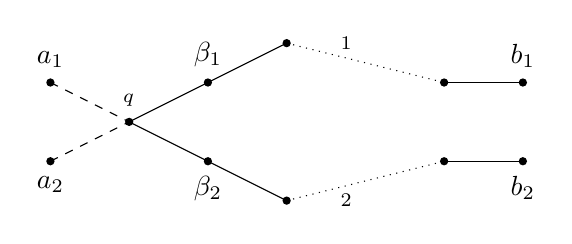
\begin{tikzpicture}

    \coordinate (a1) at (0, 0.5);
    \coordinate (a2) at (0, -0.5);
    \coordinate (al) at (1, 0);
    \coordinate (b1) at (2, 0.5);
    \coordinate (b2) at (2, -0.5);
    \coordinate (c1) at (3, 1);
    \coordinate (c2) at (3, -1);
    \coordinate (d1) at (5, 0.5);
    \coordinate (d2) at (5, -0.5);
    \coordinate (L1) at (6, 0.5);
    \coordinate (L2) at (6, -0.5);
    
      \fill (a1) circle (1.5pt) node[above=2pt]{$a_1$};
      \fill (a2) circle (1.5pt) node[below=2pt]{$a_2$};
    \fill (b1) circle (1.5pt)  node[above=2pt]{$\beta_1$};
      \fill (b2) circle (1.5pt) node[below=2pt]{$\beta_2$};
       \fill (al) circle (1.5pt) node[above=2pt]{$\al_q$};
      \fill (c1) circle (1.5pt) node[right=16pt]{$\fP_1$};
      \fill (c2) circle (1.5pt) node[right=16pt]{$\fP_2$};
      \fill (d1) circle (1.5pt);
      \fill (d2) circle (1.5pt);
      \fill (L1) circle (1.5pt) node[above=2pt]{$b_1$};
      \fill (L2) circle (1.5pt) node[below=2pt]{$b_2$};

      
      \draw (a1) [dashed]-- (al); 
      \draw (al) -- (b1) -- (c1); 
      \draw (c1) [dotted]-- (d1); 
      \draw (d1) -- (L1); 
      \draw (a2) [dashed]-- (al);
      \draw (al) -- (b2) -- (c2); 
      \draw (c2) [dotted]-- (d2); 
      \draw (d2) -- (L2); 
    \end{tikzpicture}
    \hspace{10pt}
    \begin{tikzpicture}

    \coordinate (a1) at (0.5, 0.5);
    \coordinate (a2) at (0.5, -0.5);
    \coordinate (b1) at (2, 0.5);
    \coordinate (b2) at (2, -0.5);
    \coordinate (c1) at (3, 1);
    \coordinate (c2) at (3, -1);
    \coordinate (d1) at (5, 0.5);
    \coordinate (d2) at (5, -0.5);
    \coordinate (L1) at (6, 0.5);
    \coordinate (L2) at (6, -0.5);
    
      \fill (a1) circle (1.5pt) node[above=2pt]{$a_1$};
      \fill (a2) circle (1.5pt) node[below=2pt]{$a_2$};
    \fill (b1) circle (1.5pt)  node[above=2pt]{$\beta_1$};
      \fill (b2) circle (1.5pt) node[below=2pt]{$\beta_2$};
  
      \fill (c1) circle (1.5pt) node[right=16pt]{$\fP_1'$};
      \fill (c2) circle (1.5pt) node[right=16pt]{$\fP_2'$};
      \fill (d1) circle (1.5pt);
      \fill (d2) circle (1.5pt);
      \fill (L1) circle (1.5pt) node[above=2pt]{$b_1$};
      \fill (L2) circle (1.5pt) node[below=2pt]{$b_2$};

      \draw (a1) [dashed]-- (b1);
      \draw (b1) -- (c1); 
      \draw (c1) [dotted]-- (d1); 
      \draw (d1) -- (L1); 
      \draw (a2) [dashed]-- (b2);
      \draw (b2) -- (c2); 
      \draw (c2) [dotted]-- (d2); 
      \draw (d2) -- (L2); 
    \end{tikzpicture}
    \caption{Illustration of the construction of paths $\fP_1'$ and $\fP_2'$ (right panel) from $\fP_1$ and $\fP_2$ (left panel).}\label{Fig:construct2B2}
  \end{figure}
  
%On the other hand, we define paths $\fP'_1=([\al_q]\to [b_1])$ and $\fP_2'=([\al_q]\to [b_2])$ in the new graph as the paths obtained by removing the edges $([\al_q],[\beta_{1}])$ and $([\al_q],[\beta_{2}])$, and then adding the ghost edges $([a_1],[\beta_1])$ and $([a_2],[\beta_2])$ to the paths $\fP_1$ and $\fP_2$, respectively. 



Note that $\cal G^{\mathrm{new}}_{\ba\bfb}$ defined above is also a graph satisfying the assumptions in \Cref{lem:Anp_key_gh}, but with one fewer internal vertex and two fewer solid edges compared to the original graph $\cal G_{\ba\bfb}$. Therefore, by the induction hypothesis, we can bound it by 
\begin{align*}
\sum_{\bal'} \cal G^{\mathrm{new}}_{\ba\bfb}(\bal') \prec &~ (W^d\eta_t)^{-(q-1)}  \cdot \Psi_t^{\ord(\cal G^{\mathrm{new}}_{\ba\bfb})-n_{\ngh}(\cal G^{\mathrm{new}}_{\ba\bfb})} \cdot  \prod_{i=3}^p  [\Psi_t(c|a_i-b_i|)]^{\chi(\fP_i)} \nonumber\\
= &~ (W^d\eta_t)^{-(q-1)}\cdot \Psi_t^{\ord(\cal G_{\ba\bfb})-n_{\ngh}(\cal G_{\ba\bfb})}\cdot  \prod_{i=1}^p  [\Psi_t(c|a_i-b_i|)]^{\chi(\fP_i)}, \end{align*}
where, in the second step, we use that $\ord(\cal G^{\mathrm{new}}_{\ba\bfb})=\ord(\cal G_{\ba\bfb})$, $n_{\ngh}(\cal G^{\mathrm{new}}_{\ba\bfb})=n_{\ngh}(\cal G_{\ba\bfb})$, and $\chi(\fP_1)=\chi(\fP_2)=0$. 
Thus, we can bound the LHS of \eqref{kwuyayw} as follows: 
\begin{align}\label{kwuyayw_case3}
\sum_{\bal\in \bD_{\bpi}} \cal G_{\ba\bfb}(\bal) &\prec \sum_{\bal'} \cal G^{\mathrm{new}}_{\ba\bfb}(\bal')\sum_{\al_q}\xi_{\al_q\beta_1}\xi_{\al_q\beta_2} \prec (W^d\eta_t)^{-1}\sum_{\bal'} \cal G^{\mathrm{new}}_{\ba\bfb}(\bal') \nonumber\\
&\prec (W^d\eta_t)^{-q}\cdot \Psi_t^{\ord(\cal G_{\ba\bfb})-n_{\ngh}(\cal G_{\ba\bfb})}\cdot  \prod_{i=1}^p  [\Psi_t(c|a_i-b_i|/2)]^{\chi(\fP_i)} ,
\end{align}
where we use the Cauchy-Schwarz inequality and \eqref{eq:Gbyxi3} in the second step. This implies \eqref{kwuyayw} in Case (III). 





% For this case, we also define a new graph $\Gamma'$, whose vertices are 
% $$
% z_1\cdots z_{p-1}, \quad a_1,a_2, a_3\cdots a_m, \quad b_1,\cdots b_m
% $$
% It has the same $k$-th ($k\ge 3$) paths as those in $\Gamma$. For the $i$-th ($i=1,2$) path in $\Gamma'$, we define them as follows. First let's say $z_p$ connecting with $x_1$ and $x_2$ besides $a_1$ and $a_2$ in the 1st and 2nd path in  $\Gamma$, i.e,. 
% $$
% x_1-z_p-a_1, \quad x_2-z_p-a_2
% $$
% In $\Gamma'$, we keep the  $x_i$-to-$b_i$ part of the $i-th$ path in $\Gamma$. Then add two ghost edges  $\overline{x_ia_i}$ 


% Then   
% $$\sum_{z_1\cdots z_p} \chi_\pi \cdot Val (\Gamma)\prec \sum_{z_1\cdots z_{p-1}}\left(Val (\Gamma')\cdot\sum_{z_p} f_K(z_p,x_1)\cdot f_K(z_p,x_2) \right)
% $$
% We have: 
% $$\sum_{z_p} f_K(z_p,x_1)\cdot f_K(z_p,x_2)\prec\eta^{-1}
% $$
% Note, the follow quantities clearly did not change from $\Gamma$ to $\Gamma'$

% \begin{enumerate}
%     \item The degree  of $z_i$ ($1\le i\le p-1$) 
%     \item Whether a path has ghost edge or not. 
%     \item The number of paths pass through $\{z_i: i\in A\subset [[1,p-1]]\}$ for any fixed $A$
% \end{enumerate}
% $$\left(\sum_{z_1\cdots z_{p-1}}Val (\Gamma')\right)
% \prec  \eta^{-p+1}\cdot  \prod_{s=1}^m g(\|a_{i }- b_{i}\|_K) ^{P_{ng}^{(i)}}$$
% Therefore, in this case \eqref{kwuyayw} holds.




\paragraph{\bf (IV) The remaining case}


Finally, suppose that none of Cases (I)--(III) applies. In this case, we prove \eqref{kwuyayw} directly, without using the induction hypothesis. (Note that we cannot argue by counting the ending edges attached to internal vertices: a path may pass through external vertices, so that some of its ending edges are not incident to any internal vertex, and the number $q$ of internal vertices may be smaller than $p$.)

First, let $K$ be the number of edges of $\cal G_{\ba\bfb}$. We further partition $\bD_{\bpi}$ into at most $K^p$ subregions according to which edge of each path $\fP_i$ without a ghost edge is the longest one; it suffices to prove \eqref{kwuyayw} with $\bD_{\bpi}$ replaced by any of these subregions. On such a subregion, by the triangle inequality, the chosen edge of $\fP_i$ has length at least $|a_i-b_i|/K$, so it contributes a factor $\Psi_t(c|a_i-b_i|)$ with $c=1/K$ by \eqref{eq:Gbyxi3}. We bound the chosen edge of each path without a ghost edge in this way and remove it from the graph, and we also remove all ghost edges. Let $\cal H$ denote the resulting graph, which contains only solid edges, and let $n_s(\cal H)=\ord(\cal G_{\ba\bfb})+2q-n_{\ngh}(\cal G_{\ba\bfb})$ be the number of its solid edges. Since all graph values are nonnegative, we may then sum over all $\bal\in(\Zn)^q$, so \eqref{kwuyayw} follows from
\begin{align}\label{kwuyayw_ng}
        \sum_{\bal\in (\Zn)^q} \cal H(\bal) \prec (W^d\eta_t)^{-q}\cdot \Psi_t^{n_s(\cal H)-2q}.
    \end{align}
The key to proving \eqref{kwuyayw_ng} is to construct a \emph{nested order of summation} for the $q$ internal vertices, as in \cite{yang2021random}: when we sum over the internal vertices in this order, each vertex being summed over must be incident to at least two solid edges whose other endpoints are external vertices or internal vertices that have not yet been summed over. Summing over such a vertex yields a factor $(W^d\eta_t)^{-1}$ by the Cauchy-Schwarz inequality and \eqref{eq:Gbyxi3}, while all other solid edges incident to it are bounded by $\Psi_t$. Hence, the existence of such an order implies \eqref{kwuyayw_ng}.

We first observe that, for every nonempty subset $A$ of the internal vertices,
\be\label{eq:degali}
e_{\cal H}(A,A^c)\ge |A| \quad \text{and}\quad \#\{\text{solid edges of }\cal H\text{ incident to }A\}\ge 2|A|,
\ee
where $A^c$ is the set of all other (internal or external) vertices, and $e_{\cal H}(A,A^c)$ is the number of solid edges of $\cal H$ between $A$ and $A^c$. Indeed, removing one edge from each path $\fP_i$ splits it into two edge-disjoint segments, each of which starts at an external vertex ($a_i$ or $b_i$), and every vertex of $\fP_i$ lies on one of them. If $\fP_i$ passes through $A$, then one of its two segments enters $A$ from $A^c$, which gives a solid edge between $A$ and $A^c$; since the paths are edge-disjoint, the first bound in \eqref{eq:degali} follows from property (3) of \Cref{lem:Anp_key}. For the second bound, by property (2) of \Cref{lem:Anp_key}, every internal vertex $\al\in A$ lies on segments of at least two distinct paths, and each of these segments contains the edge through which it reaches $\al$ for the first time; these edges are incident to $A$ and are distinct for distinct pairs (segment, vertex).

We now construct the order backwards, i.e., we first determine the vertex that is summed over last. Let $\mathscr A$ denote the set consisting of the external vertices and of the internal vertices chosen so far. As long as there is an internal vertex $\al\notin\mathscr A$ with at least two solid edges to $\mathscr A$, we add it to $\mathscr A$. Suppose that this procedure stops while the set $A$ of the remaining internal vertices is nonempty. Then, each $\al\in A$ has at most one solid edge to $A^c=\mathscr A$, so by the first bound in \eqref{eq:degali} it has exactly one such edge, which we denote by $(\al,x_\al)$. Let $\cal C$ be a connected component of the subgraph of $\cal H$ induced on $A$. Applying the second bound in \eqref{eq:degali} to $\cal C$, we see that $\cal C$ contains at least $|\cal C|$ edges, and hence a cycle (possibly consisting of two parallel edges). We pick two vertices $\al,\beta\in\cal C$ that are adjacent on this cycle and use
\be\label{kwuyayw_ng_tree}
\xi_{\al x_\al}\,\xi_{\beta x_\beta}\le \frac12\left(\xi_{\al x_\al}^2+\xi_{\beta x_\beta}^2\right) .
\ee
Consider the graph in which $\xi_{\al x_\al}\xi_{\beta x_\beta}$ is replaced by $\xi_{\al x_\al}^2$ (the other term is treated in the same way, with the roles of $\al$ and $\beta$ exchanged). In this graph, $\al$ has two edges to $\mathscr A$, so it can be added to $\mathscr A$. Next, every vertex of $\cal C\setminus\{\beta\}$ that is adjacent to $\mathscr A$ has two edges to $\mathscr A$ (its edge to $x_\cdot$ and an edge to an added vertex), so all vertices connected to $\al$ in $\cal C\setminus\{\beta\}$ can be added one by one. These include both neighbors of $\beta$ on the cycle, so $\beta$ can be added as well, and then the remaining vertices of $\cal C$ can be added one by one along paths in $\cal C$ starting from $\beta$. Applying \eqref{kwuyayw_ng_tree} to one such pair in each connected component of the subgraph induced on $A$, we obtain $\OO(1)$ many graphs, for each of which the procedure exhausts all internal vertices; see \Cref{Fig:construct_trees} for an illustration. Since \eqref{kwuyayw_ng_tree} does not change the number of solid edges, summing over the internal vertices in the reverse order of their addition proves \eqref{kwuyayw_ng}, and hence \eqref{kwuyayw} in Case (IV). (In fact, this argument does not use the assumption that Cases (I)--(III) do not apply.)
\begin{figure}[h]
    \centering
    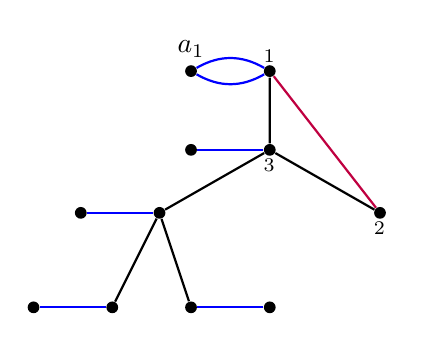
\begin{tikzpicture}[scale=2, every node/.style={circle, fill=black, inner sep=1.5pt}]
  % Nodes
 \node (A) at (0,0) {};       % root
\node[anchor=south,draw=none,fill=none] at (A) {$\al_1$};
  \node (B) at (0,-0.5) {};  
  \node[anchor=north,draw=none,fill=none] at (B) {$\al_3$};
  \node (C) at (-0.7,-0.9) {};     
  \node (D) at (-1,-1.5) {};  
  \node (E) at (-0.5,-1.5) {};    
  \node (F) at (0.7,-0.9) {};  
  \node[anchor=north,draw=none,fill=none] at (F) {$\al_2$};

\node (A1) [left of = A, distance=4pt] {};
\node[anchor=south,draw=none,fill=none] at (A1) {$a_1$};
\node (B1) [left of = B, distance=4pt] {};  
\node (C1) [left of = C, distance=4pt] {};
\node (D1) [left of = D, distance=4pt] {};
\node (E1) [right of = E, distance=4pt] {};
%\node (F1) [right of = F, distance=4pt] {};
%\node[anchor=north,draw=none,fill=none] at (F1) {$[a_2]$};

  % Black edges (tree structure)
  \draw[black, thick] (A) -- (B) -- (C) -- (D);
  \draw[black, thick] (C) -- (E);
  \draw[black, thick] (B) -- (F);
  \path [draw=blue, thick] (A) to [bend left] (A1); 
  \path [draw=blue, thick] (A) to [bend right] (A1); 
  %\draw[red, thick, bend left] (A) -- (A1);
  \draw[blue, thick] (B) -- (B1);
  \draw[blue, thick] (C) -- (C1);
  \draw[blue, thick] (D) -- (D1);
  \draw[blue, thick] (E) -- (E1);
  \draw[purple, thick] (A) -- (F);

\end{tikzpicture}
    \hspace{10pt}
    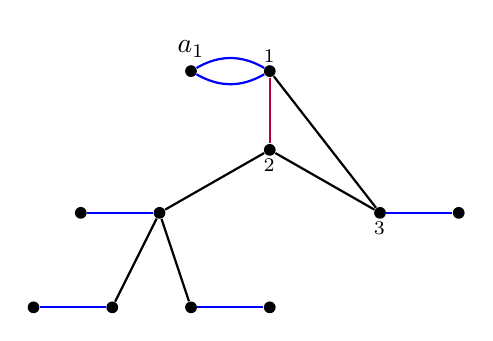
\begin{tikzpicture}[scale=2, every node/.style={circle, fill=black, inner sep=1.5pt}]
  % Nodes
  \node (A) at (0,0) {};       % root
\node[anchor=south,draw=none,fill=none] at (A) {$\al_1$};
  \node (B) at (0,-0.5) {};  
\node[anchor=north,draw=none,fill=none] at (B) {$\al_2$};
  \node (C) at (-0.7,-0.9) {};     
  \node (D) at (-1,-1.5) {};  
  \node (E) at (-0.5,-1.5) {};    
  \node (F) at (0.7,-0.9) {};
  \node[anchor=north,draw=none,fill=none] at (F) {$\al_3$};

\node (A1) [left of = A, distance=4pt] {};
\node[anchor=south,draw=none,fill=none] at (A1) {$a_1$};
%\node (B1) [right of = B, distance=4pt] {};  
\node (C1) [left of = C, distance=4pt] {};
\node (D1) [left of = D, distance=4pt] {};
\node (E1) [right of = E, distance=4pt] {};
\node (F1) [right of = F, distance=4pt] {};



  % Black edges (tree structure)
  \draw[purple, thick] (A) -- (B);
  \draw[black, thick] (A) -- (F);
  \draw[black, thick] (C) -- (D);
  \draw[black, thick] (C) -- (B);
  \draw[black, thick] (C) -- (E);
  \draw[black, thick] (B) -- (F);
  \path [draw=blue, thick] (A) to [bend left] (A1); 
  \path [draw=blue, thick] (A) to [bend right] (A1); 
  %\draw[red, thick, bend left] (A) -- (A1);
  %\draw[blue, thick] (B) -- (B1);
  \draw[blue, thick] (C) -- (C1);
  \draw[blue, thick] (D) -- (D1);
  \draw[blue, thick] (E) -- (E1);
  \draw[blue, thick] (F) -- (F1);

\end{tikzpicture}
\caption{Two examples of a connected component $\cal C$ in Case (IV), after the splitting \eqref{kwuyayw_ng_tree} with $(\al,\beta)=(\al_1,\al_2)$, in the term containing $\xi_{\al_1 a_1}^2$. Blue edges represent the solid edges to the set $\mathscr A$, here to external vertices (blue is used solely for illustration and does not indicate the $+$ charge of $G$-edges as in \Cref{def_graph1}); the purple edge is the edge between $\al_1$ and $\al_2$ on a cycle of $\cal C$; and black edges represent the other solid edges inside $\cal C$. The vertex $\al_1$ is added to $\mathscr A$ first; every other vertex except $\al_2$ is added as soon as it is adjacent to $\mathscr A$, and $\al_2$ is added once two of its neighbors belong to $\mathscr A$.}\label{Fig:construct_trees}
  \end{figure}

 \end{proof}

% Now, due to the previous two cases, we know that if a $z$ vertex connects with three or more ending edges, then it either be two short ending edges case, or two long ending edges case. Therefore, any $z$ vertex only connects at most two ending edges.  There are at least $p$ paths passing through $z$ vertices, and there two ending edges connect with these $z_1\cdots z_p$ vertices. Therefore, the only possible case (which we have not discussed) is the one with the following properties

% \begin{enumerate}
% \item There are exactly $p$ paths passing through $z_1\cdots z_p$.
%     \item each $z_i$ connects with two ending edges
%     \item for the ending edges connecting with $z_i$, one is $A1$ or $B1$ type, another one is $B2$.
% \end{enumerate}
% We notice that there are $p$ $B2$ ending edges in the $p$ paths. Therefore, all of these $p$ paths have ghost edges, i.e., for all $1\le i\le p$, 
% $$
% P_{ng}^{(i)}=0
% $$

% It implies that there is \textbf{no $A1$ types. } More precisely,  each $z_i$ connects with two ending edges, one is $B1$ type, another one is $B2$.

% Now each $z_i$ should connect with exactly two other edges, therefore, these edges form loops (with $z$ as vertices). Wlog, we can assume that there is only 1 loop connecting $z_i$'s like 
% $$
% z_1-z_2-z_3\cdots z_p-z_1$$

% Wlog, we assume that the $B1$ type ending edge connecting with $z_i$ is $\overline {z_ia_i}$. Therefore, we only need to prove that 
% $$
% \sum_{z_1\cdots z_p}\left(\prod_{i=1}^pf(z_i,a_i)\right)
% \left(\prod_{i=1}^pf(z_i,z_{i+1})\right)\prec \eta^{-p}
% $$
% The trick is applying Schwarz inequality on $\prod_{i=1}^2f(z_i,a_i)$,
% $$
% \prod_{i=1}^2f(z_i,a_i)\le \sum_i f^2(z_i,a_i)
% $$
% By symmetric, we only need to prove that 
%  $$
% \sum_{z_1\cdots z_p}f^2(z_1,a_1)\cdot \left(\prod_{i=3}^pf(z_i,a_i)\right)
% \left(\prod_{i=1}^pf(z_i,z_{i+1})\right)\prec \eta^{-p}
% $$
% To see that, one only needs to do the sum with the order $z_2$ (first), then $z_3,z_4\cdots z_p$ and $z_1$ (last).  Done. 


%\subsubsection*{\bf The mixed case: general} 
% So far, we have reduced to the case that there is no $z$'s connecting with two or more short ending edges in this graph. But we know there are at least $p$ short ending edges and there are $p$ $z$ vertices. It implies the following key result:
%  \begin{enumerate}
%      \item  Each $z_i$ connects with exactly one short ending edge, more precisely $B1$ edge. 
%      \item There are exactly $p$ paths and all of them have ghost edge. 
%  \end{enumerate}
%  Then we only need to prove 
%  $$
%  \sum_{z_1\cdots z_p} Val (\Gamma)\prec \eta^{-p}
%  $$
% More precisely, we only need to create a net without using ghost edge.  Now we reset the graph as follows: 
%  \begin{enumerate}
%      \item For each $z_i$, it connects with $a_i$ and it is a $B1$ edge. 
%      \item The other non-ghost edges are $z-z$ edges.  
%  \end{enumerate}
% Now we look at one special case: 
% $$
% \deg_{non-ghost} (z_i)=2$$
% Note, $\deg_{non-ghost} (z_i)$ is impossible to be less than 2. If it is equal to $2$, with $\deg (z_i)\ge 4$, it must connect with two ghost edges, then it can be reduced to simple case as abvoe two long ending edge case. 
% Therefore we can assume that 
% $$
% \deg_{non-ghost} (z_i)\ge 3
% $$






\subsection{Proof of Lemma \ref{lem:LW_moment_exp}}\label{subsec_pf_LW_moment_exp}

Note that when $|a-b|\le (\log W)^{3/2}\ell_t$ or $\ell\le (\log W)^{3/2}\ell_t$, $\sT_{t}(|a-b|\wedge \ell)$ does not exhibit exponential decay. In this regime, \Cref{lem:LW_moment_exp} follows directly from \Cref{lem:LW_moment}. Therefore, for the remainder of the proof, it suffices to establish \eqref{eq:LW_moment_exp} under the conditions  
\be\label{eq:far_ab_K}
|a-b|> (\log W)^{3/2}\ell_t,\quad \text{and}\quad (\log W)^{3/2}\ell_t\le \ell \le (\log W)^{10}\ell_t.
\ee
For this purpose, we decompose $f_{xy}(G)=f_{xy}^{>\ell}(G)+f_{xy}^{\le \ell}(G)$ into two parts, where
\begin{align*}
f_{xy}^{>\ell}(G)&=W^{-d}\sum_{a_1:|a_1-a|\wedge |a_1-b|>\ell}\sum_{a_2}S^{(\sB)}_{a_1a_2}\sum_{\substack{\al\in[a_2],\beta \in[a_1],\\ \al\notin\{x,y\}}}
\Gc_{\beta\beta} G_{x\al }G_{\al y},\\
f_{xy}^{\le \ell}(G)&=f_{xy}^{(a)}(G)+f_{xy}^{(b)}(G),\quad f_{xy}^{(a)}(G):=W^{-d}\sum_{a_1:|a_1-a|\le \ell}\sum_{a_2}S^{(\sB)}_{a_1a_2}\sum_{\substack{\al\in[a_2],\beta \in[a_1],\\ \al\notin\{x,y\}}}
\Gc_{\beta\beta} G_{x\al }G_{\al y},
\end{align*}
and $f_{xy}^{(b)}(G)$ is defined in the same way as $f_{xy}^{(a)}(G)$, with the summation over $a_1$ restricted to $|a_1-a|> \ell\ge |a_1-b|$.
\Cref{lem:LW_moment_exp} follows immediately from the next two estimates on \(f_{xy}^{>\ell}(G)\) and \(f_{xy}^{\le \ell}(G)\) with $\Psi_t = (W^{-d}B_{t,0})^{1/2}$:

\begin{lemma}\label{lem:LW_moment_exp_far}
In the setting of \Cref{lem:LW_moment_exp}, for any fixed $p\in 2\N$, the following estimate holds for any large constant $D>0$:
\be\label{eq:LW_moment_exp_far}
\E\big|f_{xy}^{>\ell}(G)\big|^{p}\prec \frac{1}{\eta_t^p} \Psi_t^p \cdot \br{\sT_{t}(|a-b|\wedge \ell) }^{p}+W^{-D}.
\ee
\end{lemma}
\begin{lemma}\label{lem:LW_moment_exp_near}
In the setting of \Cref{lem:LW_moment_exp}, for any fixed $p\in 2\N$, the following estimate holds for any large constant $D>0$:
\be\label{eq:LW_moment_exp_near}
\E\big|f_{xy}^{\le \ell}(G)\big|^{p}\prec \frac{1}{\eta_t^p} \Psi_t^p \cdot \br{\sT_{t}(|a-b|\wedge \ell) }^{p}+W^{-D}. 
\ee
\end{lemma}



First, the proof of \Cref{lem:LW_moment_exp_far} is similar to that for \Cref{lem:LW_moment}.
\begin{proof}[\bf Proof of \Cref{lem:LW_moment_exp_far}]
First, similar to \Cref{lem:localregular}, we expand $\big|f_{xy}^{>\ell}(G)\big|^{p}$ into a sum of locally standard graphs satisfying properties (1)--(6) listed there. Next, we bound each locally standard graph using its associated auxiliary graph, constructed as in \Cref{def_auxgraph}.
We then estimate the auxiliary graphs using a result analogous to \Cref{lem:Anp_key}. More precisely, suppose \smash{$\cal G^{\aux}_{\ba\bfb}$} is a nested graph that satisfies the assumptions of \Cref{lem:Anp_key}. In addition, all internal vertices lie in the domain  $\bD_{>\ell}:=\{c \in \Zn:|a_i-c|\wedge |b_i-c|> \ell \ \text{ for all } i\in\qqq{p}\}$. Indeed, every vertex created by the local expansions is connected to an existing vertex by a path of dotted or waved edges (see the discussion below \Cref{T eq0}), so every internal molecule contains one of the vertices $\beta\in[a_1]$ of the $p$ factors $f_{xy}^{>\ell}(G)$ or $\overline{f_{xy}^{>\ell}(G)}$, and we choose such a vertex as the center of the molecule in \Cref{def_auxgraph}. Then, we aim to show that
\begin{equation}\label{adsuu33}
\cal G^{\aux}_{\ba\bfb} \prec (W^d\eta_t)^{-q}\cdot \Psi_t^{\ord(\cal G^{\aux}_{\ba\bfb})-p}\cdot \br{\sT_{t}(|a-b|\wedge \ell) }^{p}+W^{-D} .
\end{equation}
In the proof of \Cref{lem:Anp_key_gh}, each path contributed at least one factor of $\Psi_t(c|a_i-b_i|)$ because, roughly speaking, every path contains at least one long ending edge. In the current setting, where $a_i=[a]$ and $b_i=[b]$ for all $i\in\qqq{p}$, we use the fact that the first edge of each path $\fP_i$ is ``long'': it joins $[a]$ either to $[b]$, in which case its length is $|a-b|$, or to an internal vertex, in which case its length is larger than $\ell$, since all internal vertices lie in the domain $\bD_{>\ell}$.
Since each solid edge $\xi([\al],[\beta])$ is bounded by $\sT_t(|[\al]-[\beta]|\wedge\ell)+W^{-D}$ and $\sT_t$ is decreasing, each such long edge provides a factor of $\sT_t(|a-b|\wedge\ell)$ (up to a negligible error $W^{-D}$), and we can treat it as a type-A2 edge. Replacing these A2 edges with ghost edges in all paths $\fP_i$, $i\in \qqq{p}$, yields a total factor of $\br{\sT_{t}(|a-b|\wedge\ell)}^{p}$. For the remaining graph---denoted by \(\cal G^{\new}_{\ba\bfb}\)---we need to establish the following bound for any constant $D>0$:
\begin{equation}\label{adsuu44}
\cal G^{\new}_{\ba\bfb} \prec (W^d\eta_t)^{-q}\cdot \Psi_t^{\ord(\cal G^{\new}_{\ba\bfb})} +W^{-D} .
\end{equation}
The proof of this estimate follows exactly the same argument as in \Cref{lem:Anp_key_gh}, and we omit the details.
\end{proof}

For the proof of \Cref{lem:LW_moment_exp_near}, we need a new argument that makes use of the exponential decay in $\sT_t$. 
\begin{proof}[\bf Proof of \Cref{lem:LW_moment_exp_near}]
Since $|f_{xy}^{\le \ell}(G)|^p\le 2^{p-1}(|f_{xy}^{(a)}(G)|^p+|f_{xy}^{(b)}(G)|^p)$, it suffices to bound $\E|f_{xy}^{(a)}(G)|^{p}$; the term $f_{xy}^{(b)}(G)$ is handled in the same way, with $a$ replaced by $b$ in the definition of the domain $\bD_{\le\ell}$ below.
Similar to \Cref{lem:localregular}, we expand $\big|f_{xy}^{(a)}(G)\big|^{p}$ into a sum of locally standard graphs satisfying properties (1)--(6) listed there.
Next, we bound each locally standard graph using its associated auxiliary graph, constructed as in \Cref{def_auxgraph}. This yields a class of auxiliary graphs \smash{$\cal G^{\aux}_{[a][b]}$} satisfying the assumptions of \Cref{lem:Anp_key} with $[a_i]=[a]$ and $[b_i]=[b]$ for $i\in \qqq{p}$. Moreover, choosing the centers of the internal molecules as in the proof of \Cref{lem:LW_moment_exp_far}, all internal vertices of the graph lie in the domain $\bD_{\le \ell}:=\{c \in \Zn:|a-c|\le \ell\}$. It remains to bound such graphs as follows: % with $\Psi_t=(W^{-d}B_{t,0})^{1/2}$:  
\begin{equation}\label{adsuu_exp}
\cal G^{\aux}_{[a][b]} \prec (W^d\eta_t)^{-q}\cdot \Psi_t^{\ord(\cal G^{\aux}_{[a][b]})-p}\cdot \br{\sT_{t}(|[a]-[b]|\wedge \ell)}^{p}+W^{-D} .
\end{equation}

We first control \smash{$\cal G^{\aux}_{[a][b]}$} by bounding each solid edge, say $\xi([\al],[\beta])$, by its upper bound $\sT_t(|[\al]-[\beta]|\wedge \ell)+W^{-D}$. 
Discarding the negligible error term containing $W^{-D}$ factors, we obtain a new graph, denoted by \smash{${\mathscr G}_{[a][b]}$}, which has the same graphical structure as \smash{$\cal G^{\aux}_{[a][b]}$} but with each solid edge representing a $\sT_t$ factor instead. Hence, to prove \eqref{adsuu_exp}, it suffices to establish that
\begin{equation}\label{adsuu_exp2}
\mathscr G_{[a][b]} = \sum_{\bal=([\al_1],\ldots,[\al_q])\in (\bD_{\le \ell})^q}\mathscr G_{[a][b]}(\bal) \prec (W^d\eta_t)^{-q}\cdot \Psi_t^{\ord(\mathscr G_{[a][b]})-p}\cdot \br{\sT_{t}(|[a]-[b]|\wedge \ell)}^{p} ,
\end{equation}
where, recall, \smash{$\mathscr G_{[a][b]}(\bal)$} denotes the graph obtained by fixing the external vertices to $\bal$, and $\ord(\mathscr G_{[a][b]})$ is defined in \eqref{eq:ordGaux}.
%denotes the number of solid edges in \smash{$\mathscr G_{[a][b]}$}. 
To show \eqref{adsuu_exp2}, we sum over the internal vertices in $\bal$ one by one. Unlike in the proof of \Cref{lem:Anp_key}, the order of summation here is arbitrary; for definiteness, we follow the order $[\al_1],\ldots,[\al_q]$. At each step, we apply the following key estimate.
\begin{claim}\label{claim:TTk}
Assume $1-t\ge \ilambda^2/L^{2}$. Then, for any $k \ge 2$ and any $0\le \ell \le (\log W)^{10}\ell_t$, the following bound holds with $\Psi_t=(W^{-d}B_{t,0})^{1/2}$:\footnote{This estimate can be viewed as an extension of \Cref{lem:propT} in the regime $1-t \ge \ilambda^2/L^2$, except that here we obtain a ``$\prec$'' bound, rather than the ``$\lesssim$'' bound in \eqref{TTT2}, due to the presence of additional logarithmic factors.}
\begin{align}\label{eq:key_T_reudce}
 \sum_{[\al]\in \bD_{\le \ell}} \prod_{i=1}^k \br{\sT_{t}(|[x_i]-[\al]|\wedge \ell) \cdot \sT_{t}(|[y_i]-[\al]|\wedge \ell) } \prec (W^{d}\eta_t)^{-1} \cdot {\Psi_t^{k-2}} \cdot   \prod_{i=1}^k \sT_{t}(|[x_i]-[y_i]|\wedge \ell) .
\end{align}
\end{claim}

 
We defer the proof of \Cref{claim:TTk} to \Cref{pf:claim_TTk}, where it is derived from elementary calculus estimates. (That proof only uses that $\bD_{\le\ell}$ is contained in a ball of radius $\ell$ in $\Zn$.)
%cite \cite{DYYY25_d3} here
The estimate \eqref{eq:key_T_reudce} shows that when summing over an internal vertex $[\al]$, each path of the form $([x_i]\to [\al]\to [y_i])$ consisting of two solid edges through $[\al]$ is effectively replaced by a single solid edge $[x_i]\to [y_i]$ in the resulting graph. We refer to this as the ``path-preserving phenomenon''. In addition, the summation over $[\al]\in \bD_{\le \ell}$ contributes a factor $(W^d\eta_t)^{-1}$ from each such pair of solid edges, along with the factor $\Psi_t^{k-2}$ reflecting the reduction in scaling order. Note that the case $k=2$ is critical---the estimate \eqref{eq:key_T_reudce} fails when $k=1$. \Cref{Fig:construct_keepT} illustrates the path-preserving phenomenon in the critical case $k=2$.

  \begin{figure}[h]
    \centering
    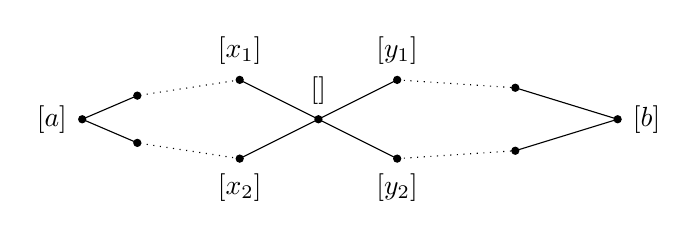
\begin{tikzpicture}
    \coordinate (L) at (-2, 0);
    \coordinate (x1) at (-1.3, 0.3);
    \coordinate (x2) at (-1.3,- 0.3);
    \coordinate (a1) at (0, 0.5);
    \coordinate (a2) at (0, -0.5);
    \coordinate (al) at (1, 0);
    \coordinate (b1) at (2, 0.5);
    \coordinate (b2) at (2, -0.5);
    %\coordinate (c1) at (3, 1);
    %\coordinate (c2) at (3, -1);
    \coordinate (d1) at (3.5, 0.4);
    \coordinate (d2) at (3.5, -0.4);
    \coordinate (R) at (4.8, 0);
   %\coordinate (R) at (6, -0.5);

    \fill (L) circle (1.5pt) node[left=2pt]{$[a]$};
    \fill (x1) circle (1.5pt) node[above=2pt]{};
      \fill (x2) circle (1.5pt) node[below=2pt]{};
      \fill (a1) circle (1.5pt) node[above=2pt]{$[x_1]$};
      \fill (a2) circle (1.5pt) node[below=2pt]{$[x_2]$};
    \fill (b1) circle (1.5pt)  node[above=2pt]{$[y_1]$};
      \fill (b2) circle (1.5pt) node[below=2pt]{$[y_2]$};
       \fill (al) circle (1.5pt) node[above=2pt]{$[\al]$};
      %\fill (c1) circle (1.5pt) node[right=16pt]{$\fP_1$};
      %\fill (c2) circle (1.5pt) node[right=16pt]{$\fP_2$};
      \fill (d1) circle (1.5pt);
      \fill (d2) circle (1.5pt);
      \fill (R) circle (1.5pt) node[right=2pt]{$[b]$};
      %\fill (L2) circle (1.5pt) node[below=2pt]{$[b_2]$};

      \draw (L) -- (x1); 
      \draw (L) -- (x2); 
      \draw (a1) [dotted]-- (x1); 
      \draw (a2) [dotted]-- (x2); 
      \draw (a1) -- (al); 
      \draw (a2) -- (al); 
      \draw (al) -- (b1); 
      \draw (b1) [dotted]-- (d1); 
      \draw (d1) -- (R); 
      \draw (al) -- (b2);
      \draw (b2) [dotted]-- (d2); 
      \draw (d2) -- (R); 
    \end{tikzpicture}
    \hspace{10pt}
    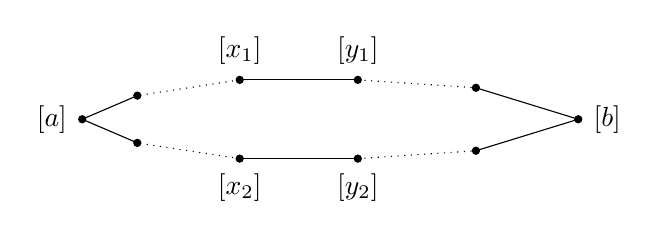
\begin{tikzpicture}
    \coordinate (L) at (-2, 0);
    \coordinate (x1) at (-1.3, 0.3);
    \coordinate (x2) at (-1.3,- 0.3);
    \coordinate (a1) at (0, 0.5);
    \coordinate (a2) at (0, -0.5);
    %\coordinate (al) at (1, 0);
    \coordinate (b1) at (1.5, 0.5);
    \coordinate (b2) at (1.5, -0.5);
    %\coordinate (c1) at (3, 1);
    %\coordinate (c2) at (3, -1);
    \coordinate (d1) at (3, 0.4);
    \coordinate (d2) at (3, -0.4);
    \coordinate (R) at (4.3, 0);
   %\coordinate (R) at (6, -0.5);

    \fill (L) circle (1.5pt) node[left=2pt]{$[a]$};
    \fill (x1) circle (1.5pt) node[above=2pt]{};
    \fill (x2) circle (1.5pt) node[below=2pt]{};
    \fill (a1) circle (1.5pt) node[above=2pt]{$[x_1]$};
    \fill (a2) circle (1.5pt) node[below=2pt]{$[x_2]$};
    \fill (b1) circle (1.5pt)  node[above=2pt]{$[y_1]$};
    \fill (b2) circle (1.5pt) node[below=2pt]{$[y_2]$};
    %\fill (al) circle (1.5pt) node[above=2pt]{$[\al_q]$};
      %\fill (c1) circle (1.5pt) node[right=16pt]{$\fP_1$};
      %\fill (c2) circle (1.5pt) node[right=16pt]{$\fP_2$};
    \fill (d1) circle (1.5pt);
    \fill (d2) circle (1.5pt);
    \fill (R) circle (1.5pt) node[right=2pt]{$[b]$};
      %\fill (L2) circle (1.5pt) node[below=2pt]{$[b_2]$};

      \draw (L) -- (x1); 
      \draw (L) -- (x2); 
      \draw (a1) [dotted]-- (x1); 
      \draw (a2) [dotted]-- (x2); 
      \draw (a1) -- (b1); 
      \draw (a2) -- (b2); 
      %\draw (al) -- (b1); 
      \draw (b1) [dotted]-- (d1); 
      \draw (d1) -- (R); 
      %\draw (a2) [dashed]-- (al);
     % \draw (al) -- (b2);
      \draw (b2) [dotted]-- (d2); 
      \draw (d2) -- (R); 
    \end{tikzpicture}
    \caption{Illustration of the path-preserving phenomenon in applying \eqref{eq:key_T_reudce}.}\label{Fig:construct_keepT}
  \end{figure}

%Key: Add in version 2 {\cor Draw a graph to illustrate the above process.}


We perform the summations of $\mathscr G_{[a][b]}$ over the internal vertices by generating a sequence of new graphs that consistently satisfy conditions (1)--(3) in \Cref{lem:Anp_key} with $[a_i]\equiv [a]$ and $[b_i]\equiv [b]$. To illustrate this procedure, consider the summation over $[\al_1]$. Suppose there are $k_1$ two-edge paths passing through $[\al_1]$ in $\mathscr G_{[a][b]}$. More precisely, assume that each path $\fP_i$ can be decomposed as
\[([a_i]\too [x_{i,1}]\to [\al_1] \to [y_{i,1}] \too [x_{i,2}]\to[\al_1]\to [y_{i,2}]\too \cdots \too [x_{i,r_{i}}]\to[\al_1]\to [y_{i,r_{i}}]\too [b_i]),\]
where we omit intermediate vertices on the path and only list those vertices $[x_{i,j}]$ and $[y_{i,j}]$ that are directly connected to $[\al_1]$, and $r_i\ge 0$ is a non-negative integer. Then, we apply \eqref{eq:key_T_reudce} to the summation 
\begin{align}\nonumber
 \sum_{[\al_1]\in \bD_{\le \ell}} \prod_{i=1}^p\prod_{j=1}^{r_i}  \br{\sT_{t}(|[x_{i,j}]-[\al_1]|\wedge \ell) \cdot \sT_{t}(|[y_{i,j}]-[\al_1]|\wedge \ell)} ,
\end{align}
which yields the bound
\[\sum_{[\al_1]\in \bD_{\le \ell}}\mathscr G_{[a][b]}(\bal) \prec (W^d\eta_t)^{-1} \Psi_t^{k_1-2} \cdot \mathscr G^{(1)}_{[a][b]}([\al_2],\ldots,[\al_q]) ,\] 
where $k_1$ is defined as $k_1=\sum_{i=1}^p r_i$, %we have used $W^{-d/2}\le \Psi_t$, 
and \smash{$\mathscr G^{(1)}_{[a][b]}$} is a new graph obtained by removing the vertex $[\al_1]$ from $\mathscr G_{[a][b]}$ and replacing each pair of solid edges $([x_{i,j}]\to[\al_1]\to [y_{i,j}])$ by $([x_{i,j}], [y_{i,j}])$.  
It is easy to see that the new graph \smash{$\mathscr G^{(1)}_{[a][b]}$} also satisfies conditions (1)--(3) in \Cref{lem:Anp_key}. Next, summing over the vertex $[\al_2]$ in \smash{$\mathscr G^{(1)}_{[a][b]}$} gives another graph \smash{$\mathscr G^{(2)}_{[a][b]}([\al_3],\ldots,[\al_q])$} that again satisfies conditions (1)--(3) in \Cref{lem:Anp_key}, along with a factor $(W^d\eta_t)^{-1} \Psi_t^{k_2-2}$ for some $k_2\ge 2$. 
Continuing this procedure, after summing over all internal vertices, we can bound the LHS of \eqref{adsuu_exp2} as  
\[\sum_{\bal\in (\bD_{\le \ell})^q}\mathscr G_{[a][b]}(\bal)\prec (W^d\eta_t)^{-q}\cdot \Psi_t^{\ord(\mathscr G_{[a][b]})-p}\cdot \mathscr G^{(q)}_{[a][b]},\]
where \smash{$\mathscr G^{(q)}_{[a][b]}$} is a graph consisting solely of $p$ solid edges between $[a]$ and $[b]$, with no internal vertices. 
%Using $\Psi_t\ge W^{-d/2}$, and 
Since each solid edge is bounded by $\sT_{t}(|[a]-[b]|\wedge \ell)$, this yields \eqref{adsuu_exp2}. Combining this with \eqref{G_by_auxG} completes the proof of \Cref{lem:LW_moment_exp_near}. 
%Combining the above three cases, we conclude \eqref{eq:key_T_reudce_pf}, which further implies \eqref{eq:key_T_reudce}. 
\end{proof}



\section{Extension to the block Anderson model}\label{sec:ext-to-BA}

The proof of \Cref{MR:decol_BA} for the block Anderson model is based on the following flow framework.

\begin{lemma}[Lemma 3.3 of \cite{RBSO1D}]\label{zztE_BA}
For the block Anderson model, fix any $\ilambda>0$ and $z\in \mathbb C_+$ with $\im z\in (0, 1]$ and $\im m(z,\ilambda)\ge \kappa$. We choose %Choosing $t_0$, $E_0$, and $\ilambda_0$ as follows: 
\be\label{eq:t0E0_BA}t_0=\frac{\im m(z,\ilambda)}{\im m(z,\ilambda)+ \im z},\quad E= \frac{t_0 \re z -(1-t_0)\re m(z,\ilambda)}{\sqrt{t_0}},\quad \ilambda_0=\sqrt{t_0}\ilambda \, .\ee
Then, we have that 
 \begin{equation}\label{eq:zztE_BA}
\sqrt{t_0}m(E,\ilambda_0)=m(z,\ilambda), \ \  z_{t_0}(E,\ilambda_0) = \sqrt{t_0}z, \ \  \sqrt{t_0}M(E,\ilambda_0)=M(z,\ilambda), \ \ G(z,\ilambda) \stackrel{d}{=} \sqrt{t_0} G_{t_0;E,\ilambda_0},
 \end{equation} 
% and the following equality in distribution:
%    \begin{equation}\label{GtEGz_BA}
%     G(z,\ilambda) \stackrel{d}{=} \sqrt{t_0} G_{t_0;E,\ilambda_0},
%    \end{equation}
where recall that $G(z,\ilambda)=(H-z)^{-1}=(V+\ilambda\Psi-z)^{-1}$.
\end{lemma}
Note that $t_0\ge \kappa/(\kappa+1)$, since $\im m(z,\ilambda)\ge\kappa$ and $\im z\le 1$, and that $\im m(E,\ilambda_0)=\im m(z,\ilambda)/\sqrt{t_0}\ge\kappa$ by \eqref{eq:zztE_BA}. In particular, the flow parameters $(E,\ilambda_0)$ satisfy the bulk condition of \Cref{lem:propM} below.



%and $|E_t|\le (2-\kappa)\sqrt{t}+\oo(1)$ for $|1-t|=\oo(1)$. 
%In other words, during the flow from $t=0$ to $t_0$, the imaginary part $\eta_t$ decreases from $\eta_0\asymp 1$ to $\eta_{t_0}\asymp 1-t_0 \asymp \im z $, while the spectral parameter $z_t$ stays within the bulk of the limiting spectrum of $H_t$, provided $t\ge 1 - \e$ for a small enough constant $\e>0$ depending on $\kappa$. 


In the following proof, we fix a target spectral parameter $z=\hat{E}+\ii \eta\in \mathbf D_{\kappa,\e}$ for an arbitrarily small constant $\e>0$, where the spectral domain $\mathbf D_{\kappa,\e}$ is now defined as %(recall \eqref{eq:spectral_domain}).
\be\label{eq:spectral_domainBA}
\mathbf D_{\kappa,\e}:=\{z=\hat{E}+\ii\eta \in \C_+: \im m(z,\ilambda)\ge \kappa, N^{-1+\e}\le \eta\le 1\}.
\ee
This domain contains the spectral parameters considered in \Cref{MR:decol_BA}: if $\hat E$ satisfies the bulk condition \eqref{eq:bulkBA}, i.e., $\rho_N(\hat E)\ge\kappa$, then $\hat E+\ii\eta\in \mathbf D_{\kappa',\e}$ for all $N^{-1+\e}\le \eta\le 1$, where $\kappa'>0$ is a constant depending only on $d$, $\kappa$, and $\fd$. To see this, let $f(\eta):=\im m(\hat E+\ii\eta,\ilambda)$ for $\eta>0$, so that $f(0^+)=\pi\rho_N(\hat E)\ge\pi\kappa$. By property (4) of \Cref{lem:propM} below, $|f'(\eta)|\le (2f(\eta)^2)^{-1}$, hence $f(\eta)^3\ge (\pi\kappa)^3-3\eta/2\ge(\pi\kappa)^3/2$ for $0<\eta\le (\pi\kappa)^3/3$. For $(\pi\kappa)^3/3\le\eta\le 1$, we use that $\mu_N$, being the free convolution of the semicircle law with a probability measure supported in $[-2d\ilambda,2d\ilambda]$, is supported in $[-R,R]$ with $R:=2+2d\ilambda\le 2+2d\fd^{-1}$, and that $|\hat E|\le R$ since $\rho_N(\hat E)>0$; thus, $f(\eta)=\int \eta\,(( x-\hat E)^2+\eta^2)^{-1}\mu_N(\dd x)\ge \eta/(4R^2+1)$. Consequently, it suffices to prove the estimates in \Cref{MR:decol_BA} for $z\in\mathbf D_{\kappa,\e}$, for any fixed constant $\kappa>0$.
Accordingly, we choose the parameters $t_0$, $E$, and $\ilambda_0$ as specified in \eqref{eq:t0E0_BA}. %The second identity in \eqref{eq:E0bulk} imply that $1-t\asymp \eta_t$ uniformly in $t\in [0,t_0]$. 
Again, for simplicity of presentation, unless we want to emphasize the dependence on the flow parameters $E$ and $g_0$, we will omit them from various notations, such as $z_t(E,\ilambda_0)$, $E_t(E,\ilambda_0)$, $\eta_t(E,\ilambda_0)$, $m(E,\ilambda_0)$, $M(E,\ilambda_0)$, and $G_{t;E,\ilambda_0}\equiv G_t$. 

Since $M$ is not a multiple of the identity matrix, the block Anderson model also involves the following \emph{twisted} quantities. For $c_1,c_2\in\Zn$, let $P_{c_1c_2}$ be the $N\times N$ matrix that maps the block $[c_2]$ to the block $[c_1]$ while preserving the position inside the block, normalized in the same way as $E_a$:
\[ (P_{c_1c_2})_{xy}:=W^{-d}\,\mathbf 1\big(x\in[c_1],\ y\in[c_2],\ x-Wc_1=y-Wc_2\big),\quad\text{i.e.,}\quad P_{c_1c_2}=W^{-d}\big(\mathbf e_{c_1}\mathbf e_{c_2}^{\top}\big)\otimes I_{W^d}, \]
where $\mathbf e_{c}$ denotes the standard basis vector of $\C^{L^d}$ associated with $c\in\Zn$. In particular, $P_{cc}=E_c$, $P_{c_1c_2}^*=P_{c_2c_1}$, and $\tr(M(\sig)P_{c_1c_2})=M^{(\sB)}_{c_2c_1}(\sig)$ by \eqref{def_G0}. We refer to $\tr\big((G_t(\sig)-M(\sig))P_{c_1c_2}\big)$ as a \emph{twisted trace}, and to
\[ \wt{\cal L}_{t,\bsig,(a;c_1,c_2)}:=\tr\big(G_t(\sig_1)E_aG_t(\sig_2)P_{c_1c_2}\big),\qquad \bsig=(\sig_1,\sig_2)\in\{+,-\}^2,\ \ a,c_1,c_2\in\Zn, \]
as a \emph{twisted $2$-loop}; when $c_1=c_2$, it is the $2$-$G$-loop ${\cal L}^{(2)}_{t,\bsig,(a,c_1)}$. The deterministic approximation of $\wt{\cal L}_{t,\bsig,(a;c_1,c_2)}$ is the \emph{twisted tree}
\[ \wt{\cal K}_{t,\bsig,(a;c_1,c_2)}:=W^{-d}\sum_{a'\in\Zn}\Theta^{(\sig_1,\sig_2)}_t(a,a')\,M^{(\sB)}_{c_2a'}(\sig_1)\,M^{(\sB)}_{a'c_1}(\sig_2), \]
which coincides with ${\cal K}^{(2)}_{t,\bsig,(a,c_1)}$ in \eqref{Kn2sol} when $c_1=c_2$, and with $\wt{\cal L}_{0,\bsig,(a;c_1,c_2)}$ at $t=0$, since $G_0(\sig)=M(\sig)$. Note also that $\tr(XE_aM(\sig)P_{c_1c_2})=W^{-d}M^{(\sB)}_{ac_1}(\sig)\tr(XP_{ac_2})$ for any $N\times N$ matrix $X$; this relates twisted $2$-loops containing $\Gc_t(\sig_2)=G_t(\sig_2)-M(\sig_2)$ in place of $G_t(\sig_2)$ to $\wt{\cal L}_{t,\bsig,(a;c_1,c_2)}$ and twisted traces.
In the flow framework of \Cref{zztE_BA}, we can establish an analogue of \Cref{lem:main_ind} for the block Anderson model.


\begin{theorem}\label{lem:main_ind_BA}
In the setting of \Cref{MR:decol_BA}, fix any $z=\hat{E}+\ii \eta\in \mathbf D_{\kappa,\e}$ and consider the flow framework in \Cref{zztE_BA}. Suppose the estimates \eqref{Eq:L-KGt+IND}--\eqref{Eq:Gtlp_exp+IND} hold at some fixed $s\in [0,t_0]$, together with the following estimate at $u=s$:
\begin{itemize}
\item[(e)] {\bf Twisted-loop estimate}: We have
\be\label{eq:TL2_BA}
\max_{\bsig,a,c_1,c_2}\left|\wt{\cal L}_{u,\bsig,(a;c_1,c_2)}-\wt{\cal K}_{u,\bsig,(a;c_1,c_2)}\right|\prec \p{W^{-d}B_{u,0}}^{3/2}.
\ee
\end{itemize}
Then, there exists a constant $0<\fc_d \le 10^{-2}$ such that for any $s< t < 1$ satisfying \eqref{con_st_ind}, the estimates \eqref{Eq:L-KGt}--\eqref{Gt_bound} hold, and \eqref{eq:TL2_BA} holds at $u=t$. In addition, if $1-t\ge \ilambda^2$, then the estimate \eqref{Eq:Gdecay+s<g} holds.
%if we do not assume \eqref{Eq:Gtlp_exp+IND}, then the estimates \eqref{Eq:L-KGt}, \eqref{Eq:L-KGt2}, \eqref{Eq:Gdecay}, and \eqref{Gt_bound} still hold at $t$.
\end{theorem}

%With \Cref{lem:main_ind}, we can prove \Cref{ML:GLoop,ML:GLoop_expec,ML:GtLocal} easily by induction in $t$. The proof of \Cref{lem:main_ind} will be divided into five steps, which constitute the remainder of this paper. Throughout these steps, we assume that the assumptions of \Cref{lem:main_ind} hold. In addition, each step will build on the conclusions established in the previous steps.

With \Cref{lem:main_ind_BA} in hand, we can establish \Cref{MR:decol_BA} by induction on $t$.  

\begin{proof}[\bf Proof of \Cref{MR:decol_BA}]
By the discussion below \eqref{eq:spectral_domainBA}, it suffices to consider $z\in\mathbf D_{\kappa,\e}$. Fix $z=\hat{E}+\ii \eta\in \mathbf D_{\kappa,\e}$, and choose the flow as in \Cref{zztE_BA}. At $t=0$, we have $G_0(\sig)=M(\sig)$, so ${\cal L}^{(n)}_{0,\bsig,\ba}={\cal K}^{(n)}_{0,\bsig,\ba}$ and $\wt{\cal L}_{0,\bsig,(a;c_1,c_2)}=\wt{\cal K}_{0,\bsig,(a;c_1,c_2)}$, and the estimates \eqref{Eq:L-KGt+IND}--\eqref{Eq:Gtlp_exp+IND} and \eqref{eq:TL2_BA} hold at $s=0$. By \Cref{lem:main_ind_BA}, applying induction on $t$ from $t=0$ to $t=t_0$ (simultaneously for all target spectral parameters, see the proof of Step 1 below) yields the estimates \eqref{Eq:L-KGt}--\eqref{Gt_bound} at $t=t_0$. Using \eqref{eq:zztE_BA}, \eqref{eq:BtBt}, and \eqref{Kn2sol}, we see that these estimates together imply the entrywise local law \eqref{G_bound}, the averaged local law \eqref{G_bound_ave}, and the quantum diffusion estimates \eqref{eq:diffu1}--\eqref{Meq:QdS2} for each fixed $z$. To extend these estimates uniformly to all $z\in \mathbf D_{\kappa,\e}$, we apply a standard $N^{-C}$-net and perturbation argument. Finally, the delocalization estimate \eqref{eq:psikLinfty}, the QUE estimates \eqref{Meq:QUE} and \eqref{Meq:QUE2}, and the bulk universality \eqref{eq:universality} then follow as consequences, as shown in \Cref{subsec:main}. For the bulk universality, two modifications are needed. First, the Green's function comparison is applied with an interpolation acting only on the random part $V=H-\ilambda\Psi$, i.e., centered at the deterministic matrix $\ilambda\Psi$, as in the flow \eqref{MBM}. Second, the argument of \cite[Theorem~2.6]{YY_25} that we follow uses the analogue of \cite[Lemma~5.15]{YY_25} (cf.~\Cref{lem:improve_exp_aver}) for the matrices obtained by adding a small GUE component. For the block Anderson model, the proof of this analogue requires, in addition, a twisted averaged law for the resolvents $G$ of these matrices, namely $\max_{c_1,c_2}|\tr((G-M)P_{c_1c_2})|\prec (N\eta)^{-1}$ at the corresponding spectral parameters $z=E+\ii\eta$, for the same reason as in the proof of \Cref{lem:improve_exp_aver} below; this bound is proved in the same way as \Cref{lem:TL1_BA}.
\end{proof}


%The proof of \Cref{lem:main_ind_BA} follows the same six-step strategy outlined below \Cref{lem:main_ind}. We now describe how the arguments in \Cref{Sec:Steps12}--\ref{Sec:graph} for the random band matrix model extend to the block Anderson model. Our proof relies on the properties of the $\Theta$-propagators stated in \Cref{lem_propTH} and properties of $m(z)$ defined in \eqref{self_m} and the matrix $\sM$ defined in \eqref{def_G0}.

The proof of \Cref{lem:main_ind_BA} follows the same six-step strategy outlined below \Cref{lem:main_ind}. We now explain how the arguments in \Cref{Sec:Steps12}--\ref{Sec:graph} for the random band matrix model extend to the block Anderson model. Our proof relies on the properties of the $\Theta$-propagators stated in \Cref{lem_propTH}, together with the following properties of $m(z)$ (defined in \eqref{self_m}) and the matrix $M^{(\sB)}$ (defined in \eqref{def_G0}).


%2-$M$-loop $M^{(\sigma_1,\sigma_2)}$ stated in \Cref{lem:propM}, which were established in \cite[Lemma~3.9]{RBSO1D}.

\begin{lemma}%[Lemma 3.9 of \cite{RBSO1D}]
\label{lem:propM}
For the block Anderson model, under the condition \eqref{eq:WO}, $m=m(E,\ilambda)$ and $M^{(\sB)}=M^{(\sB)}(E,\ilambda)$ satisfy the following properties for any $E\in\R$ with $\im m(E,\ilambda)\ge \kappa$ (recall that $E$ is the spectral parameter in the flow \eqref{eq:t0E0_BA}, and that this condition holds for the flow parameters $(E,\ilambda_0)$ of \Cref{zztE_BA} when $z\in\mathbf D_{\kappa,\e}$):

\begin{enumerate}
%\item {\bf Symmetry}: $\cal M$ is symmetric, which follows from the definition \eqref{def_G0} and the fact that $\Psi$ is real symmetric. As a result, $M^{(\sigma_1,\sigma_2)}$ is also symmetric. 

% \be\label{eq:Msym}
% (M^{(\sigma_1,\sigma_2)})^\top =M^{(\sigma_2,\sigma_1)}.
% \ee

\item[(1)] {\bf Translation invariance}: For any $a,b,r\in \Zn$, we have $M^{(\sB)}_{a+r,b+r}= M^{(\sB)}_{ab}$ and $M^{(\sB)}_{aa}\equiv m$. 

%$M^{(\sig_1,\sig_2)}(a+r,b+r)= M^{(\sig_1,\sig_2)}(a,b).$
% The following block translation invariance holds: 
% \be\label{symmetryM}
%   \qquad  M^{(\sigma_1,\sigma_2)}([x]+[a],[y]+[a])= M^{(\sigma_1,\sigma_2)}([x],[y]),\ \ \forall [x],[y],[a]\in \Zn.
% \ee
% In addition, in 2D, we have the parity symmetry: 
% \be\label{symmetryP} \qquad  M^{(\sigma_1,\sigma_2)}(0,[x])= M^{(\sigma_1,\sigma_2)}([x], 0)= M^{(\sigma_1,\sigma_2)}(0,-[x]),\ \ \forall [x] \in \Zn.\ee

\item[(2)] {\bf Ward's identity}: We have \(|m|\le 1\),
\(\im m\ge \kappa\), and %the following identity
\be\label{eq:WardM}
\sum_{b}|M^{(\sB)}_{ab}|^2=1,\quad \forall a\in \Zn \, .
\ee
% \be\label{eq:propm}
% |m|\le 1, \quad \im m\gtrsim 1.
% \ee

%\item[(3)] For all $a\in \ZL$, we have
%{\bf Cauchy-Schwarz inequality}: For any $\sig_1,\sig_2\in \{+,-\}$, we have
%\be\label{eq:WardM}
%|M^{(\sigma_1,\sigma_2)}_{ab}|\le M^{(+,-)}_{ab},\quad \text{and}\quad 
%\sum_{b}|\sM_{ab}|^2=1. %,\quad \forall a,b\in \Zn,
%\ee
%where the equalities holds if $\sigma_1\ne \sigma_2$.
% Moreover, if $\sigma_1\ne \sigma_2$, we have 
% \be\label{eq:WardM1}
% \sum_{b\in\Zn}M^{(\sigma_1,\sigma_2)}_{ab} = 1,\quad \forall a\in \Zn.
% \ee

\item[(3)] {\bf Combes--Thomas bound}: There exists a constant $C>0$ (depending only on $d$ and $\kappa$) such that the following estimate holds for $\ilambda<(2C)^{-1}$: 
\begin{align}
% \label{eq:M-msc} &\|M - m_{sc}(E)I_N\|\le C\ilambda ,\quad \|M^+ - [m_{sc}(E)]^2 I_N\|_{\infty\to\infty}\le C\ilambda ,\\ 
\label{Mbound_AO}
%\|M - m_{sc}(E)I_N\|\le C\ilambda , %\quad \|M^+ - [m_{sc}(E)]^2 I_N\|_{\infty\to\infty}\le C\ilambda ,\quad 
C^{-1}\ilambda \mathbf 1(a\sim b)\le |M^{(\sB)}_{ab}|\le (C\ilambda)^{|a-b|}. 
%\quad C^{-1}\ilambda^2 \mathbf 1(a\sim b)\le \big|M^{(\sB)}_{ab}\big|^2\le (C\ilambda)^{2|a-b|}, 
\end{align}
%where $M^{(\sig_1,\sig_2)}$ is defined in \eqref{eq:Msig}. 
%where we have used \smash{$M|_{[a][b]}$} to denote the $(a,b)$-th block of $M$ following the notation in  \eqref{eq:submatrixnotation}. Furthermore, for any $\sig_1,\sig_2\in \{+,-\}$ and $a\ne b\in \Zn$, we have 
% \be\label{Mbound_AO2}
% C^{-1}\ilambda^2 \mathbf 1(a\sim b)\le \big|\big(M^{(\sig_1,\sig_2)}S^{(\sB)}\big)_{ab}\big|\le (C\ilambda)^{2|a-b|}.   
% \ee
Furthermore, for $\ilambda\ge (2C)^{-1}$, there exists a constant $c>0$ such that the following  bound holds:
\begin{align}\label{Mbound_AO2}
|M^{(\sB)}_{ab}|\le c^{-1}\exp\p{-c|a-b|}.
\end{align}

\item[(4)] {\bf Stability}: For every $z\in\C_+$ and $\ilambda>0$, with $m=m(z,\ilambda)$ and $M^{(\sB)}=M^{(\sB)}(z)$, we have
\[ \re\Big(1-L^{-d}\tr\big(M^{(\sB)}\big)^2\Big)\ge 2(\im m)^2 . \]
Consequently, $m(z,\ilambda)$ is a smooth function of $(z,\ilambda)\in\C_+\times(0,\infty)$, and
\[ |\partial_z m(z,\ilambda)|\le \frac{1}{2(\im m(z,\ilambda))^2},\qquad |\partial_{\ilambda} m(z,\ilambda)|\le \frac{d}{(\im m(z,\ilambda))^2}. \]
\end{enumerate}
\end{lemma}
\begin{proof}
Property (1) follows directly from the translation invariance of the matrix $\Psi^{(\sB)}$ in \eqref{eq:Psi3D}. The bound $\im m \ge \kappa$ is our assumption, while Ward's identity \eqref{eq:WardM} follows by taking the imaginary part of the equation \smash{$m=M^{(\sB)}_{aa}=(\ilambda \Psi^{(\sB)} - E - m)^{-1}_{aa}$}. The identity \eqref{eq:WardM} gives directly $|m|\le 1$. 
For sufficiently small $\ilambda$, the estimates in \eqref{Mbound_AO} are obtained from the Taylor expansion 
\[ M^{(\sB)} = -\sum_{k=0}^\infty (E+m)^{-k-1}(\ilambda \Psi^{(\sB)})^k.\]
For $\ilambda$ of order 1, \eqref{Mbound_AO2} is given by the classical Combes--Thomas estimate (see, e.g., \cite[Theorem 10.5]{Aizenman_book}).
For property (4), let $\psi_1,\ldots,\psi_{L^d}$ be the eigenvalues of $\Psi^{(\sB)}$ (so that $|\psi_i|\le 2d$), and let $\mu_i:=(\ilambda\psi_i-z-m)^{-1}$ be the corresponding eigenvalues of $M^{(\sB)}$. Taking the imaginary part of \eqref{self_m}, i.e., of $m=L^{-d}\sum_i\mu_i$, gives $\im m=\im(z+m)\cdot L^{-d}\sum_i|\mu_i|^2$; hence, $L^{-d}\sum_i|\mu_i|^2\le 1$ and
\[ \re\Big(1-L^{-d}\sum_i\mu_i^2\Big)\ge L^{-d}\sum_i\big(|\mu_i|^2-\re \mu_i^2\big)=2L^{-d}\sum_i(\im\mu_i)^2\ge 2\Big(L^{-d}\sum_i\im\mu_i\Big)^2=2(\im m)^2 . \]
Differentiating \eqref{self_m} with respect to $z$ and $\ilambda$, we obtain
\[ \Big(1-L^{-d}\tr\big(M^{(\sB)}\big)^2\Big)\partial_z m=L^{-d}\tr\big(M^{(\sB)}\big)^2,\qquad \Big(1-L^{-d}\tr\big(M^{(\sB)}\big)^2\Big)\partial_{\ilambda} m=-L^{-d}\tr\big(\Psi^{(\sB)}(M^{(\sB)})^2\big), \]
where the right-hand sides are bounded in absolute value by $L^{-d}\sum_i|\mu_i|^2\le 1$ and $2d$, respectively. Together with the implicit function theorem (the derivative of \eqref{self_m} with respect to $m$ does not vanish by the above stability bound), this proves property (4).
\end{proof}

Another key ingredient in the proof of \Cref{lem:main_ind_BA} is the following analogue of \Cref{lem_GbEXP}. 

\begin{lemma}\label{lem_GbEXP_BA}
In the setting of \Cref{lem:main_ind_BA}, suppose the estimates in \eqref{initialGT2} hold for a deterministic control parameter $W^{-d/2}\le \Psi_t \le W^{-\e_0}$.
%the event in \eqref{def_asGMc}. 
% In the setting of \Cref{lem:main_ind}, fix any $t\in [0,t_0]$ and suppose we have the following estimates for any $\Psi$ satisfying the assumptions \eqref{eq:Psi1D}--\eqref{sym_cond}: there exists a small constant $\e_0>0$ such that 
% \begin{equation}\label{def_asGMc2}
% \|G_t - M\|_{\max} \prec W^{-\e_0},
% \end{equation}
Furthermore, suppose there exist deterministic control parameters $0<\Phi_t(a,b)\le W^{-\e_0}$ such that  
\be\label{eq:def_Psit}
%\max_{[a],[b]\in \Zn} \cL^{(2)}_{t,(-,+),(a,b)}+W^{-d}\prec \Psi_t^2,\quad 
{\cal L}^{(2)}_{t, (-,+), (a,b)}\prec [\Phi_t(a,b)]^2,\quad \forall a,b\in \Zn .
\ee
%Then, the following estimates hold: 
\begin{itemize}
\item[(a)] {\bf Local laws}: The following entrywise and averaged local laws hold: 
    \begin{align}\label{GiiGEX_BA} 
 \|G_t-M\|_{\max} \prec \Psi_t, \quad \max_a\left|\tr \p{ \left(G_t - M\right)E_{a}}\right| \prec \Psi_t^2  . 
\end{align}

% \item[(b)] {\bf Averaged local law}: For any $a,b\in \Zn$, we have that %(recall $I_{[a]}$ defined in \eqref{def:Ia})
% \begin{align}\label{GavLGEX_BA}
% \left\langle  \left(G_t - M\right)E_{a}\right\rangle \prec \Psi_t^2 . %, \quad  W^{-d} \left\langle  \left(G_t - M\right)I_{[a]}MI_{[b]}\right\rangle  \prec \Psi_t^2\|I_{[a]}MI_{[b]}\| \, . 
% \end{align}

\item[(b)] {\bf Entrywise decay estimate}:
There exists a constant $c_{\ilambda}>0$ such that, for any large constant $D>0$ and all \(a,b\in \Zn \), the following estimate holds:
\begin{align}\label{GijGEX_BA}
\max_{x\in [a], y \in [b]} |(G_t-M)_{xy}|  \prec & \sum_{a', b' \in \Zn}  \Phi_t(a',b') e^{-c_\ilambda(|a'-a|+|b'-b|)}  + \Psi_t e^{-c_{\ilambda}|a-b|}+W^{-D} .
\end{align}
\end{itemize}
\end{lemma}
\begin{proof}
This lemma was proved as Lemma 6.1 in \cite{RBSO1D} under the condition $\ilambda\le W^{-\e}$ for a small constant $\e>0$. For $W^{-\e}<\ilambda\le\fd^{-1}$, the argument has to be modified in two places.
First, in the proof of the entrywise bounds in (a) and (b), the expansion of $M$ in powers of $\ilambda$ is replaced by the bounds \eqref{Mbound_AO} and \eqref{Mbound_AO2}, and the self-consistent equation for the diagonal entries is inverted directly in the max norm, without any expansion in $\ilambda$. Indeed, the matrix $1-tM^{(+,+)}$, $t\in[0,1]$, is diagonally dominant: its diagonal entries are equal to $1-tm^2$, while, by \eqref{eq:WardM}, its off-diagonal row sums are equal to
\[ t\sum_{b\ne a}\big|M^{(\sB)}_{ab}\big|^2=t\big(1-|m|^2\big)=\re\big(1-tm^2\big)-(1-t)-2t(\im m)^2\le \big|1-tm^2\big|-\min\{1,2\kappa^2\}, \]
where we used $\kappa\le\im m\le 1$. Hence, $\|(1-tM^{(+,+)})^{-1}\|_{\infty\to\infty}\le (\min\{1,2\kappa^2\})^{-1}$ uniformly in $t\in[0,1]$ and $0<\ilambda\le\fd^{-1}$.
Second, the averaged local law in \eqref{GiiGEX_BA} does not follow from the argument of \cite{RBSO1D} when $\ilambda\gg W^{-\e}$. Instead, we derive it from the entrywise local law by a fluctuation averaging argument for the block averages $\tr((G_t-M)E_a)$, which uses conditional expectations with respect to the independent Gaussian blocks of $V$, the bounds $|m|\le1$ and $\im m\ge\kappa$, the above stability bound, and the row bound $\max_a\sum_b|M^{(\sB)}_{ab}|\le C$ implied by \eqref{Mbound_AO} or \eqref{Mbound_AO2}. This argument does not use the smallness of $\ilambda$ and holds uniformly in $0<\ilambda\le\fd^{-1}$.
\end{proof}



\noindent{\bf Proof of Step 1 for \Cref{lem:main_ind_BA}.}
The proof of Step 1 depends on the following continuity estimates in \Cref{lem_ConArg_BA}. To make the dependence on the spectral parameter $z$ and the coupling parameter $\ilambda$ explicit, we denote the resolvent by \(G_t(z_t, \ilambda)=(V_t+\ilambda\Psi-z_t)^{-1}\) and the corresponding $G$-loop by \smash{${\cal L}^{(n)}_{t, \bsig, \ba}(z_t, \ilambda)$}, where $z_t\equiv z_t(E,\ilambda)$ is defined in \eqref{eq:zt}. %Moreover, we define the $T$-variables $(T_t)_{x\bv}(z,\ilambda)$ and \smash{$(\wt T_t)_{x\bv}(z,\ilambda)$} in terms of the resolvent $G_t(z,\ilambda)$ as in \eqref{eq:gen_T}.

\begin{lemma}\label{lem_ConArg_BA}
Fix any \( \e\le s \leq t \leq 1\) for a constant \(\e > 0\). Given any $\ilambda$ satisfying the condition \eqref{eq:WO}, let $\ilambda_s:=\ilambda\cdot \sqrt{s/t}$, and assume that $\im m(E,\ilambda_s)\ge\kappa$. Then, in the flow setting given by \Cref{def_flow} and \Cref{zztE_BA}, we have the following continuity estimates for the $G$-loops and (generalized) resolvent entries. 
\begin{enumerate}

\item Assume that the bound \eqref{eq:loopbound_s} holds at time \(s\) for the loops ${\cal L}^{(n)}_{s, \bsig, \ba}\p{z_s,\ilambda_s}$ for each fixed \(n \in \mathbb{N}\).  
% \begin{equation}\label{55}
%  \max_{\bsig, \ba} \left|{\cal L}^{(n)}_{s, \bsig, \ba}\p{z_s,\ilambda_s}\right| \prec \left( W^d \ell_{s}^d \eta_{s} \right)^{-n+1}. 
% \end{equation}
Then, on the event \(\Omega_t:=\{\|G_t(z_t,\ilambda)\|_{\max} \leq C_0\}\) for a constant $C_0>0$, the following estimate holds for any $n\ge 2$:
\begin{align}\label{res_lo_bo_eta_BA}
{\bf 1}(\Omega_t)\cdot\max_{\bsig, \ba}
\left|{\cal L}_{t, \bsig, \ba}^{(n)}\p{z_t,\ilambda}\right| \prec %\frac{\max_{[a]}\langle \im G_t(z_t,\ilambda) E_{[a]}\rangle}{\left( W^d \ell_{s}^d \eta_{t} \right)^{n-1}} =
\left(\frac{\eta_{s}}{\eta_{t}}\cdot W^{-d}B_{s,0}\right)^{n-1} .
\end{align}
% Moreover, for an arbitrary deterministic unit vector $\bv$, we have 
% \begin{align}\label{eq:cont_T}
% (T_t)_{x\bv}(z_t,\ilambda)+(\wt T_t)_{x\bv}(z_t,\ilambda) \prec (T_s)_{x\bv}(z_t,\ilambda_s)+(\wt T_s)_{x\bv}(z_t,\ilambda_s)+\frac{\ell_{t}^d}{\ell_{s}^d}\frac{\im (G_t)_{\bv\bv}(z_t,\ilambda)}{W^d \ell_{t}^d \eta_{t} }.
% \end{align}

\item Given any deterministic unit vectors $\bv,\bw\in \C^N$, suppose 
\be\label{eq:ImGs}\im (G_s)_{\bv\bv}(z_s,\ilambda_s)\lesssim 1,\quad \im (G_s)_{\bw\bw}(z_s,\ilambda_s)\lesssim 1, \quad \left|(G_s)_{\bv\bw}(z_s,\ilambda_s)\right|\lesssim 1,
\ee
with high probability, where we adopt the simplified notation of generalized matrix entries: given a matrix $\cal A$ and any vectors $\bv,\bw$, we denote $ \cal A_{\bv\bw}:= \bv^* \cal A\bw$. Then, the following estimates hold with high probability at time $t$: 
\be\label{eq:ImGt}
\im (G_t)_{\bv\bv}(z_t,\ilambda)\lesssim {\eta_s}/{\eta_t},\quad (G_t)_{\bv\bw}(z_t,\ilambda)\lesssim {\eta_s}/{\eta_t}.
\ee
 
\end{enumerate}

\end{lemma}
\begin{proof}
The proof of this lemma follows exactly the same argument as that of Lemma 7.1 in \cite{RBSO1D}, except that the factor $W^{-d}B_{s,0}$ in \eqref{res_lo_bo_eta_BA} corresponds to $(W^d\ell_s^d\eta_s)^{-1}$ therein. The assumption $\im m(E,\ilambda_s)\ge\kappa$ ensures that \Cref{lem:propM} applies to $m(E,\ilambda_s)$ and $M(E,\ilambda_s)$, which are the deterministic limits of the resolvent at time $s$; in particular, $|m(E,\ilambda_s)|\le 1$ and $\eta_t\le \kappa^{-1}\eta_s$.
\end{proof}

With \Cref{lem_GbEXP_BA,lem_ConArg_BA}, Step 1 of the proof of \Cref{lem:main_ind_BA} for the block Anderson model (i.e., the proof of \eqref{lRB1} and \eqref{Gtmwc}) is the same as that in \cite[Section 7.1]{RBSO1D}, except that \Cref{lem_ConArg_BA} is applied only with source times close to $1$. This is needed because the deterministic part $\ilambda_0\Psi$ of $H_t$ does not scale with $t$: \Cref{lem_ConArg_BA} compares the flow with parameters $(E,\ilambda_0)$ at time $u$ with the flow with parameters $(E,g')$, $g':=\ilambda_0\sqrt{s'/u}$, at an earlier time $s'$, and the latter flow must lie in the bulk. Let $c_*:=\min\{1/2,\fd\kappa^3/(6d)\}$.
\begin{itemize}
\item For $u\le 1-c_*$, we have $\eta_u=(1-u)\im m(E,\ilambda_0)\ge c_*\kappa$, hence $\|G_u\|\le (c_*\kappa)^{-1}$ and, deterministically, $|{\cal L}^{(n)}_{u,\bsig,\ba}|\le \|G_u\|^nW^{-(n-1)d}\lesssim (W^{-d}B_{u,0})^{n-1}$, since $B_{u,0}\ge(\ilambda^2+1)^{-1}$. Thus, \eqref{lRB1} holds for $u\le 1-c_*$ without using \Cref{lem_ConArg_BA}, and \eqref{Gtmwc} then follows as in the random band matrix case.

\item For $u>1-c_*$, we apply \Cref{lem_ConArg_BA} only with the source time $s':=\max(s,1-c_*)$. Then, $0\le \ilambda_0-g'\le \ilambda_0(1-s')\le c_*/\fd$, so property (4) of \Cref{lem:propM} (applied at $E+\ii\eta$, followed by the limit $\eta\downarrow 0$) gives $\im m(E,g')^3\ge \im m(E,\ilambda_0)^3-3d(\ilambda_0-g')\ge \kappa^3/2$. Hence, the source flow satisfies the assumption of \Cref{lem_ConArg_BA} with $\kappa$ replaced by $\kappa/2$. If $s'=1-c_*$, the bound \eqref{eq:loopbound_s} for the source flow at time $s'$ holds deterministically, as in the previous item.
\end{itemize}
If $s'=s$, the bound \eqref{eq:loopbound_s} for the source flow at time $s$ is provided by the induction hypothesis, in the following sense. By the scaling relations \eqref{eq:zztE_BA}, the flow with parameters $(E,g')$ at time $s$ coincides with the flow of \Cref{zztE_BA} for the coupling $g'/\sqrt{s}$ and the target spectral parameter $z':=z_{s}(E,g')/\sqrt{s}$, stopped at its final time $t_0(z')=s$. Here, $\im m(z',g'/\sqrt{s})=\sqrt{s}\,\im m(E,g')\ge\kappa/4$, so $z'\in\mathbf D_{\kappa/4,\e/2}$ for large $N$, and the coupling $g'/\sqrt{s}$ satisfies \eqref{eq:WO} up to a constant factor. Therefore, as in \cite[Section 7.1]{RBSO1D}, the induction on $t$ in the proof of \Cref{MR:decol_BA} is carried out simultaneously for all such target spectral parameters and couplings. With these modifications, we omit the details.

\medskip
\noindent{\bf Proof of Step 2 for \Cref{lem:main_ind_BA}.} 
In Step 2, the technical lemmas---\Cref{lem:newKLK,lem:LWterm,lem: EWGn2_N,lem: EMn2_N}---remain valid in the setting of the block Anderson model, except that the estimate \eqref{eq:MG_conclusion3} is modified as follows. Let ${\cal J}^{\ell}_{t,D}\ge W^{-d}$ be a \emph{deterministic} control parameter such that \smash{\(\wh{\cal J}^{\ell}_{t,D} \prec {\cal J}^{\ell}_{t,D}.\)}
% \begin{align}\label{defCALJ_deter}
% \wh{\cal J}^{\ell}_{u,D} \prec {\cal J}^{\ell}_{u,D}.
% \end{align}
Then, \eqref{eq:MG_conclusion3} continues to hold with \smash{$\wh{\mathcal{J}}_{t,D}^{\ell}$} replaced by \smash{${\mathcal{J}}_{t,D}^{\ell}$}; that is, 
\be\label{eq:MG_conclusion3_BA}
(\mathcal{E} \otimes \mathcal{E})^{M}_{t,\bsig, \ba,\ba} \prec \frac{1}{\eta_t} \left[\left(W^{-d}B_{t,0}\right)^{1/2} +  \left({\mathcal{J}}_{t,D}^{\ell}\right)^3\right]\cdot \left(W^{-d} \wT^{\ell}_{t,D}(|a-b|)\right)^2.
\ee
Assume that \eqref{Eq:Gdecay_w} holds. We combine \eqref{Kn2sol}, \eqref{Mbound_AO} (or \eqref{Mbound_AO2}), and \eqref{prop:ThfadC} to obtain \eqref{eq:kn2sol_decay}. Together with \eqref{Eq:Gdecay_w}, this yields \eqref{eq:L2_decay}. Then, applying \Cref{lem_GbEXP_BA} gives the desired estimates \eqref{Gt_bound_flow} and \eqref{Gt_avgbound_flow}.
Finally, we prove \eqref{Eq:Gdecay_w}. Using the same argument as between \eqref{lokis2} and \eqref{eq:L-K2max}, we obtain that for all $u\in[s,t]$,
\be\label{eq:L-K2max_BA} \max_{\bsig,\ba}\left|\left({\cal L}-{\cal K}\right)^{(2)}_{u,\bsig,\ba}\right|\prec 
 \p{\frac{1-s}{1-u}}^{C_0+\frac54}(W^{-d}B_{u,0})^{\frac 5 4} \le (W^{-d}B_{u,0})^{\frac1 5}\cdot \p{W^{-d} \widetilde{\cal {T}}^{\ell^{(0)}}_{u,D}\p{|a-b|}},
\ee
where $\ell^{(0)}=0$ as chosen in \eqref{ksjjuw}. Next, we implement a similar inductive argument as that below \eqref{ksjjuw}: assume that \eqref{kwr3juw} holds for length scales $K_u$ satisfying \eqref{eq:monotone_Ku}.
Moreover, suppose we have the initial estimate
\be\label{eq:Gronwall_dervJuD_BA}
\wh{\mathcal{J}}_{u,D}^{K_u} \prec \mathcal{J}_{u,D}^{K_u}, \ \ \ \forall u\in [s,t], \quad \text{where}\quad \mathcal{J}_{u,D}^{K_u}\equiv (W^{-d}{B}_{t,0})^{\frac{1}{50}}.    
\ee
We then define the stopping time 
\be\label{eq:def2_stopping_BA} 
\tau :=t\wedge T,\quad \text{with}\quad T:=\inf\left\{u\ge s: \wh{\cal J}_{u,D}^{K_u} \ge (W^{-d}B_{u,0})^{\frac1{100}} \right\}.\ee
By \Cref{lem: EWGn2_N}, the estimate \eqref{eq:boundGcterm} remains valid.
On the other hand, using \eqref{eq:MG_conclusion3_BA} together with \Cref{lem:DIfREP}, the estimate \eqref{eq:boundmgterm} becomes
\be\label{eq:boundmgterm_BA}
\begin{split}
\int_s^\tau \dd \mathcal{E}^{M}_{u, \bsig, {\ba}} &\prec  \Big[\left(W^{-d}B_{\tau,0}\right)^{1/4}  + \sup_{u\in[s,\tau]}\p{{\cal J}_{u,D}^{K_u}}^{3/2}\Big]\cdot \left(W^{-d} \wT^{K_\tau}_{\tau,D}(|a-b|)\right) .\end{split}
\ee
Applying the same reasoning as below \eqref{eq:boundmgterm} and invoking Gr{\"o}nwall's inequality, we obtain
\be\label{eq:Gronwall_dervJuD_BA2}
\wh{\mathcal{J}}_{u,D}^{K_u} \prec\left(\frac{1-s}{1-u}\right)^{C_0}\br{(W^{-d} {B} _{t,0})^{1/5} + \p{{\cal J}_{t,D}^{K_t}}^{3/2} },\quad \forall u\in [s,\tau].  
\ee
This implies that $T\ge t$ with high probability, so \eqref{eq:Gronwall_dervJuD_BA2} holds for all $u\in [s,t]$. We then take the RHS of \eqref{eq:Gronwall_dervJuD_BA2} as the new control parameter $\mathcal{J}_{u,D}^{K_u}$ and repeat the above argument. Iterating this procedure $\OO(1)$ times yields the improved bound 
\be\label{eq:Gronwall_dervJuD_BA3}
\wh{\mathcal{J}}_{u,D}^{K_u} \prec\left(|1-s|/|1-u|\right)^{C_0}(W^{-d} {B} _{t,0})^{1/5},\quad \forall u\in [s,t].  
\ee
Next, we redefine the scale $K_u'$ as in \eqref{eq:def_ell1}. Under this choice, using \eqref{eq:Gronwall_dervJuD_BA3}, we can re-establish the initial estimate \eqref{eq:Gronwall_dervJuD_BA} with $K_u$ replaced by $K_u'$, provided the constant $\fc_d$ in \eqref{con_st_ind} is chosen sufficiently small.
Finally, repeating the above procedure $\OO(1)$ more times yields \eqref{Eq:Gdecay_w} at $u=t$. The same argument clearly applies to all $u\in [s,t]$. 

It remains to justify the validity of \Cref{lem:newKLK,lem:LWterm,lem: EWGn2_N,lem: EMn2_N} for the block Anderson model. First, the proof of \Cref{lem:newKLK} in \Cref{subsec:pf_lem:newKLK} carries over with only a minor modification: in the derivation of \eqref{uu2j2ois}, we additionally make use of \eqref{Mbound_AO} or \eqref{Mbound_AO2}. 
The proofs of \Cref{lem:LWterm,lem: EWGn2_N} require more substantial changes in the graphical tools, which will be detailed in \Cref{subsec:LWchange-to-BA} below. 
Finally, the proof of \Cref{lem: EMn2_N} (with \eqref{eq:MG_conclusion3} replaced by \eqref{eq:MG_conclusion3_BA}) follows the same argument as in \Cref{subsec:pf_lem: EMn2_N}, with the following adjustments:

\begin{proof}[\bf Proof of \Cref{lem: EMn2_N} for the block Anderson model]
Most of the arguments in \Cref{subsec:pf_lem: EMn2_N} carry over directly to the block Anderson model, provided we can establish the following resolvent estimate under the assumption \eqref{eq:LW_assm}: for any $a,b\in \Zn$ and $x\in[a]$, $y\in [b]$, 
\begin{equation}\label{eq_resolventunderpoly}
|(G_t-M)_{xy}| \prec \Psi_t(|a-b|).
\end{equation}
To prove \eqref{eq_resolventunderpoly}, we apply \eqref{GijGEX_BA} to obtain
\begin{align*}
|(G_t-M)_{xy}|   \prec \sum_{|a'-a|\vee |b'-b| \le (\log W)^{3/2}}\Psi_t(|a'-b'|)e^{-c_\ilambda(|a'-a|+|b'-b|)} + \Psi_t(0)e^{-c_{\ilambda}|a-b|} + W^{-D} \prec \Psi_t(|a-b|) ,  
\end{align*}
where $D>0$ is an arbitrarily large constant. Here, in the second step, we have used the conditions in \eqref{eq:Psi} to obtain that %for sufficiently large $D$,
\be\label{eq:Psirelations}\begin{aligned}
    &\Psi_t(|a'-b'|)\prec \Psi_t(|a-b|) ,\quad \Psi_t(|a-b|)\gtrsim C_1^{-1}\p{|a-b|+1}^{-C_2}\Psi_t(0)\ge W^{-D},\\  
    &\Psi_t(0)e^{-c_{\ilambda}|a-b|} \lesssim C_1^{-1}(|a-b|+1)^{-C_2}\Psi_t(0) \lesssim \Psi_t(|a-b|).
\end{aligned}
\ee
Under the stronger assumption \eqref{eq:LW_assm_exp}, a parallel argument yields the following analogue of \eqref{eq_resolventunderpoly}:
\begin{equation}\label{eq_resolventunderexp}
|(G_t-M)_{xy}| \prec \big(W^{-d} \wT_{t,D}^{\ell}(|a-b|) \big)^{1/2},\quad \forall x\in [a], y\in [b].
\end{equation}


We now prove \eqref{eq:MG_conclusion} using the estimate \eqref{eq_resolventunderpoly}. As in \eqref{eq:S1+S2}, we need to bound 
\[\cal S_1:= W^d \sum_{|c-b|> |c-a|}  \mathcal{L}^{(6)}_{t, (\bsig\otimes \bsig)^{(1)}, \ba(c,c)},\quad \cal S_2:= W^d \sum_{|c-b|\le |c-a|} \mathcal{L}^{(6)}_{t, (\bsig\otimes \bsig)^{(1)}, \ba(c,c)}. \]
By symmetry, it suffices to establish \eqref{eq:MG_conclusion} for $\mathcal{S}_1$. %Analogous to \eqref{eq_S1_bound}, 
In this case, we apply \eqref{eq_sym_loop_bound} with $c'=c$ to get that 
\begin{equation}\label{eq_S1_bound_BA}
    \mathcal{S}_1 \lesssim \frac{1}{\eta_t}\max_{|c-b| \ge |a-b|/2} \left(\mathcal{L}^{(4)}_{t,\bsig^{(\alt)}, (c,b,c,b)}\right)^{1/2} \cdot  \max_{\sig\in\{+,-\}} \big|\mathcal{L}^{(3)}_{t, (\sigma,\sig_2,-\sig_2), (a,b,a)} \big|. %\mathcal{L}^{(4)}_{t, \bsig', (a,b,a,c)}.
\end{equation}
We write the $(c,b,c,b)$-loop as 
\[\mathcal{L}^{(4)}_{t,\bsig^{(\alt)}, (c,b,c,b)}=W^{-4d} \sum_{z',z''\in[c]}\sum_{y_1,y_2\in [b]} G_{y_1 z'}(\sig_1) G_{z'y_2}(-\sig_1) G_{y_2 z''} (\sig_1)G_{z''y_1}(-\sig_1).\]
Expanding each resolvent entry as 
\be\label{eq:G+G-M}
G_{\al \beta}(\sig)=M_{\al \beta}(\sig)+(G-M)_{\al\beta}(\sig),\quad \forall \al,\beta\in \{y_1,y_2,z',z''\}, \ \sig\in\{+,-\},\ee 
we bound every $(G-M)_{\al\beta}$ using \eqref{eq_resolventunderpoly} and each $M_{\al \beta}$ using \eqref{Mbound_AO} or \eqref{Mbound_AO2}. This yields (with $\e>0$ a small constant): 
\begin{align*}
   \mathcal{L}^{(4)}_{t,\bsig^{(\alt)}, (c,b,c,b)} &\prec \Psi_t^4(|b-c|)+\br{W^{-d}\Psi_t^3(|b-c|)+ W^{-2d}\Psi_t^2(|b-c|) + W^{-3d}\Psi_t(|b-c|)+W^{-3d}} e^{-\e|b-c|} \\
  & \lesssim \Psi_t^4(|b-c|) \lesssim \Psi_t^4(|a-b|),
\end{align*}
where the second step uses a bound analogous to \eqref{eq:Psirelations}, and the last step follows from $|c-b|\ge |a-b|/2$ together with the condition \eqref{eq:Psi}. 
Inserting this bound into \eqref{eq_S1_bound_BA}, we obtain the estimate \eqref{eq:reduce4to3} again.
% \begin{equation}\label{eq:reduce4to3_BA}
%     \mathcal{S}_1 \prec W^d \Psi_t^2\left(|a-b|\right) \sum_{c} \mathcal{L}^{(4)}_{t, \bsig', (a,b,a,c)}\prec \frac{1}{\eta_t} \Psi_t^2\left(|a-b|\right) \max_{\sig\in\{+,-\}}\left|\mathcal{L}^{(3)}_{t, (\sig,\sig_2,-\sig_2), (a,b,a)}\right|,
% \end{equation} 
% where, in the second step, we applied Ward's identity \eqref{WI_calL}. 
To handle the 3-loop on the RHS of \eqref{eq:reduce4to3}, we again expand each resolvent entry as in \eqref{eq:G+G-M}, bound every $(G-M)_{\al\beta}$ with \eqref{eq_resolventunderpoly}, and each $M_{\al \beta}$ with \eqref{Mbound_AO} or \eqref{Mbound_AO2}. This gives the same bound as in \eqref{eq:reduce4_bdd3}, 
% \begin{align}
%  \mathcal{L}^{(3)}_{t, (\sig,\sig_2,-\sig_2), (a,b,a)}& \prec \Psi_t(0)\cdot \Psi_t^2(|a-b|)+ \Psi_t(0)\cdot W^{-d}W^{-\e|a-b|}\cdot \Psi_t(|a-b|)+ W^{-2d} W^{-\e|a-b|} \nonumber\\   
%  &\lesssim \Psi_t(0) \cdot \Psi_t^2(|a-b|),\label{eq:reduce4_bdd3_BA}
% \end{align} 
where the factor $ \Psi_t^2(|a-b|)$ comes from the entries $G_{x'y}$ and $G_{yx}$ between blocks $a$ and $b$, while the short leg $G_{xx'}$ contributes a factor $\Psi_t(0)+W^{-d}\lesssim\Psi_t(0)$ by \eqref{GiiGEX_BA}. (Specifically, $(G-M)_{xx'}$ contributes $\Psi_t(0)$, while the deterministic part $M_{xx'}$ yields a factor $W^{-d}$.) %via the $(\infty\to \infty)$-norm bound in \eqref{Mbound_AO}.} 
Substituting \eqref{eq:reduce4_bdd3} into \eqref{eq:reduce4to3} concludes  \eqref{eq:MG_conclusion}.

Next, the exponential decay bound \eqref{eq:MG_conclusion3_BA} can be established by an argument analogous to that used for \eqref{eq:MG_conclusion3} below \eqref{eq:cutoff_scales}. 
First, it follows directly from the polynomial decay bound \eqref{eq:MG_conclusion} whenever \smash{$|a-b| \le \ell_t^{\dag}$}. It therefore remains to consider the case \eqref{eq:largea-b}, where we must control the three terms \smash{\(\widetilde{\mathcal{S}}_i\)}, $i\in \{1,2,3\}$, appearing in \eqref{eq;S123} with $c'=c$. The terms \smash{$\widetilde{\mathcal{S}}_1$ and $\widetilde{\mathcal{S}}_2$} can be bounded by the same argument used between \eqref{eq:pointwise_loop2} and \eqref{eq:boundwtS_1}, except that here we apply \eqref{eq_resolventunderexp} in place of the estimates \eqref{GijGEX} and \eqref{eq:LW_assm_exp} employed there.
For the term \smash{$\wt {\cal S}_3$}, we bound all legs of the original $6$-$G$-loop directly using \eqref{GijGEX_BA} together with the control parameter \smash{$\cal J_{t,D}^{\ell}$}. In this setting, \eqref{eq_L2-J} remains valid with \smash{$\wh{\cal J}_{t,D}$} replaced by \smash{$\cal J_{t,D}^{\ell}$}, where the $2$-$\cK$-loop \smash{$\mathcal{K}^{(2)}_{t,(-,+),(a,b)}$} defined in \eqref{Kn2sol} is of order $\OO(W^{-D})$ thanks to the exponential decay of the $\Theta$-propagators in \eqref{prop:ThfadC} and the decay of the $2$-$M$-loop due to \eqref{Mbound_AO} or \eqref{Mbound_AO2}. Using \eqref{eq_L2-J} (with \smash{$\wh{\cal J}_{t,D}^{\ell}$} replaced by $\cal J_{t,D}^{\ell}$) and an argument analogous to that below \eqref{eq_resolventunderpoly}, we obtain that for any $x\in [a]$ and $y\in [b]$ with $|a-b|\gtrsim\ell_t^*$,
\begin{equation}\label{eq_resolventunderexp2}
|(G_t-M)_{xy}| \prec \big(W^{-d} \wT_{t,D}^{\ell}(|a-b|) \big)^{1/2} \implies |(G_t)_{xy}| \prec \big(W^{-d} \wT_{t,D}^{\ell}(|a-b|) \big)^{1/2},
\end{equation}
where the implication uses the bound \eqref{Mbound_AO} or \eqref{Mbound_AO2}.
Finally, combining \eqref{eq_resolventunderexp2} with the same reasoning as below \eqref{eq_L2-J}, we conclude the exponential decay bound \eqref{eq:MG_conclusion3_BA}.
\end{proof}



\noindent{\bf Proof of Steps 3--6 for \Cref{lem:main_ind_BA}.} 
The proofs in \Cref{Sec:Steps34,Sec:Step5,Sec:Step6} extend verbatim to the block Anderson model, except for the arguments in \Cref{sec:Step5_larget}, the proof of \Cref{lem:improve_exp_aver}, and the proof of \Cref{lem:LWterm_EXP}. In \Cref{sec:Step5_larget}, the random band matrix case relies on \Cref{lem_GbEXP} and follows the approach of \cite[Section 5.3]{YY_25}, whereas the corresponding arguments for the block Anderson model are based on \Cref{lem_GbEXP_BA} and parallel those in \cite[Section 7.3]{RBSO1D}. We therefore omit the details.
The proof of \Cref{lem:LWterm_EXP} is deferred to \Cref{subsec:pf-LWterm_EXP} below.
In Step 6, i.e., in the proofs of \Cref{lem:improve_exp_aver,lem:LWterm_EXP}, we use in addition the following twisted averaged law, which is a consequence of Steps 2 and 3, and the twisted-loop estimate \eqref{eq:TL2_BA} for $u\in[s,t]$, which we derive after Step 4 below.

\begin{lemma}[Twisted averaged law]\label{lem:TL1_BA}
In the setting of \Cref{lem:main_ind_BA}, suppose that the estimates \eqref{Gt_bound_flow}, \eqref{Gt_avgbound_flow}, and \eqref{Eq:LGxb} with $n\le 4$ hold at some $u\in[s,t]$. Then, we have
\[ \max_{\sig\in\{+,-\}}\max_{c_1,c_2\in\Zn}\Big|\tr\Big(\big(G_u(\sig)-M(\sig)\big)P_{c_1c_2}\Big)\Big|\prec W^{-d}B_{u,0} . \]
In particular, this bound holds uniformly in $u\in[s,t]$ after Steps 2 and 3.
\end{lemma}
\begin{proof}
Since $\tr((G_u^*-M^*)P_{c_1c_2})=\overline{\tr((G_u-M)P_{c_2c_1})}$, it suffices to consider $\sig=+$. Denote $\delta_b:=\tr((G_u-M)E_b)$ and $\Lambda:=\max_{c_1,c_2}|\tr((G_u-M)P_{c_1c_2})|$. By \eqref{def_G0} and \eqref{eq:zt}, we have $H_u-z_u=V_u+M^{-1}+u\,m$, where $V_u:=H_u-H_0$. Together with $\cal S[M]=mI_N$, this gives the identity
\be\label{eq:GminusM_BA}
G_u-M=-M\,\underline{V_uG_u}+u\,M\,\cal S[G_u-M]\,G_u,\qquad \underline{V_uG_u}:=V_uG_u+u\,\cal S[G_u]\,G_u ,
\ee
where $\cal S[G_u-M]=W^d\sum_b\delta_bE_b$ by \eqref{eq:opS} and \eqref{bandcwV}. Multiplying \eqref{eq:GminusM_BA} by $P_{c_1c_2}$ and taking the trace, we obtain from $M=M^{(\sB)}\otimes I_{W^d}$ that
\[ \tr\big((G_u-M)P_{c_1c_2}\big)=-\tr\big(M\underline{V_uG_u}P_{c_1c_2}\big)+u\sum_b\delta_bM^{(\sB)}_{c_2b}M^{(\sB)}_{bc_1}+u\sum_b\delta_bM^{(\sB)}_{c_2b}\tr\big((G_u-M)P_{c_1b}\big). \]
By \eqref{Gt_avgbound_flow}, the Cauchy--Schwarz inequality, and \eqref{eq:WardM}, the second term on the right-hand side is $\prec W^{-d}B_{u,0}$. By \eqref{Gt_avgbound_flow} and the row bound $\max_c\sum_b|M^{(\sB)}_{cb}|\le C$, which follows from \eqref{Mbound_AO} or \eqref{Mbound_AO2}, the third term is $\prec W^{-d}B_{u,0}\cdot\Lambda$. Since $W^{-d}B_{u,0}\le W^{-c}$ for a constant $c>0$ by \eqref{eq:WO}, this term can be absorbed into the left-hand side after taking the maximum over $c_1,c_2$.

It remains to show that $X:=\tr(M\underline{V_uG_u}P_{c_1c_2})\prec W^{-d}B_{u,0}$, which follows from a high-moment estimate. Applying Gaussian integration by parts to the entries of $V_u$ in one factor $X$ of $\E|X|^{2p}$, $p\in\N$, the term in which the derivative acts on the resolvent in the same factor is cancelled by the renormalization in $\underline{V_uG_u}$. In the remaining terms, the derivative acts on one of the other $2p-1$ factors, and, using \eqref{eq:GminusM_BA} again (i.e., $\underline{V_uG_u}=-M^{-1}(G_u-M)+u\,\cal S[G_u-M]G_u$), it produces sums of products of resolvent entries with deterministic weights. The leading one is $u\sum_{x,w}S_{xw}(G_uP_{c_1c_2}M)_{wx}(G_uP_{c_1c_2}M)_{xw}$ (or its analogue with one factor replaced by its complex conjugate). Since $(G_uP_{c_1c_2}M)_{wx}=W^{-d}M^{(\sB)}_{c_2[x]}(G_u)_{w\tilde x}$, where $\tilde x\in[c_1]$ has the same position inside its block as $x$, the Cauchy--Schwarz inequality and \eqref{eq:WardM} bound it by
\[ u\,W^{-d}\sum_b\big|M^{(\sB)}_{c_2b}\big|^2\,{\cal L}^{(2)}_{u,(+,-),(b,c_1)}\prec (W^{-d}B_{u,0})^2 , \]
where we used \eqref{Eq:LGxb} with $n=2$. The other terms are bounded in the same way, using \eqref{Gt_bound_flow} and \eqref{Eq:LGxb} with $n\le 4$, by $(W^{-d}B_{u,0})^{2}$ times a product of $2p-2$ factors $X$ or $\overline X$. This yields $\E|X|^{2p}\prec (W^{-d}B_{u,0})^{2}\,\E|X|^{2p-2}$, and hence $X\prec W^{-d}B_{u,0}$ by H{\"o}lder's and Markov's inequalities, since $p$ is arbitrary.
\end{proof}

\medskip
\noindent{\bf Proof of the twisted-loop estimate \eqref{eq:TL2_BA} for $u\in[s,t]$.}
Fix $\bsig=(\sig_1,\sig_2)$ and $c_1,c_2\in\Zn$, and regard $Z_u(a):=\wt{\cal L}_{u,\bsig,(a;c_1,c_2)}-\wt{\cal K}_{u,\bsig,(a;c_1,c_2)}$ as a vector indexed by $a\in\Zn$. The derivation of the loop hierarchy \eqref{eq:mainStoflow} by It{\^o}'s formula does not use the special form of the matrices $E_{a_i}$, so it also applies to $\wt{\cal L}_{u,\bsig,(a;c_1,c_2)}$, viewed as a $2$-loop in which $E_{a_2}$ is replaced by $P_{c_1c_2}$. Since $S^{(\sB)}=I_{L^d}$, the cut-and-glue term in \eqref{eq:mainStoflow} then becomes $W^d\sum_{b}{\cal L}^{(2)}_{u,\bsig,(a,b)}\wt{\cal L}_{u,\bsig,(b;c_1,c_2)}$. On the other hand, since $\partial_u\Theta^{(\sig_1,\sig_2)}_u=\Theta^{(\sig_1,\sig_2)}_uM^{(\sig_1,\sig_2)}\Theta^{(\sig_1,\sig_2)}_u$, we have $\partial_u\wt{\cal K}_{u,\bsig,(a;c_1,c_2)}=W^d\sum_{b}{\cal K}^{(2)}_{u,\bsig,(a,b)}\wt{\cal K}_{u,\bsig,(b;c_1,c_2)}$ by \eqref{Kn2sol}. Hence, with the evolution kernel $\wt{\cal U}_{v,u}:=\Theta^{(\sig_1,\sig_2)}_u(\Theta^{(\sig_1,\sig_2)}_v)^{-1}$ acting on the index $a$, we have
\be\label{eq:Duhamel_twist}
Z_u=\wt{\cal U}_{s,u}Z_s+\int_s^u\wt{\cal U}_{v,u}\Big(\wt{\cal B}_{1,v}+\wt{\cal B}_{2,v}+\wt{\cal E}^{\Gc}_v\Big)\dd v+\int_s^u\wt{\cal U}_{v,u}\,\dd\wt{\cal E}^{M}_v ,
\ee
where $\wt{\cal B}_{1,v}(a):=W^d\sum_b(\cL-\cK)^{(2)}_{v,\bsig,(a,b)}\wt{\cal K}_{v,\bsig,(b;c_1,c_2)}$ and $\wt{\cal B}_{2,v}(a):=W^d\sum_b(\cL-\cK)^{(2)}_{v,\bsig,(a,b)}Z_v(b)$, while $\wt{\cal E}^{\Gc}_v$ and $\dd\wt{\cal E}^{M}_v$ are the light-weight and martingale terms defined as in \eqref{def_EwtG} and \eqref{def_Edif}, with $E_{a_2}$ replaced by $P_{c_1c_2}$. In particular, $\wt{\cal E}^{\Gc}_v(a)$ is a sum of twisted $3$-loops $\tr(G_v(\sig_1)E_{b}G_v(\sig_1)E_aG_v(\sig_2)P_{c_1c_2})$ and $\tr(G_v(\sig_1)E_{a}G_v(\sig_2)E_bG_v(\sig_2)P_{c_1c_2})$, multiplied by $W^d\tr(\Gc_v(\sig_i)E_{b})$ and summed over $b$.

We reduce twisted loops to $G$-loops using the following two facts. First, by the Cauchy--Schwarz inequality, for any $N\times N$ matrices $X_1,X_2$,
\[ \big|\tr\big(X_1E_aX_2P_{c_1c_2}\big)\big|^2\le\tr\big(E_{c_2}X_1E_aX_1^*\big)\,\tr\big(E_aX_2E_{c_1}X_2^*\big); \]
for example, $|\wt{\cal L}_{v,\bsig,(a;c_1,c_2)}|^2\le{\cal L}^{(2)}_{v,(\sig_1,-\sig_1),(a,c_2)}\,{\cal L}^{(2)}_{v,(\sig_2,-\sig_2),(a,c_1)}$. Second, since $G-G^*=2\ii\eta GG^*=2\ii\eta G^*G$ and $\sum_aE_a=W^{-d}I_N$, we have the Ward identity
\[ \sum_a\wt{\cal L}_{v,(\sig,-\sig),(a;c_1,c_2)}=\frac{1}{2\ii W^d\eta_v}\Big(\tr\big(G_vP_{c_1c_2}\big)-\tr\big(G_v^*P_{c_1c_2}\big)\Big),\quad \sig\in\{+,-\}, \]
and the same identity holds for $\wt{\cal K}$, with $\tr(G_vP_{c_1c_2})$ and $\tr(G_v^*P_{c_1c_2})$ replaced by $M^{(\sB)}_{c_2c_1}$ and $(M^{(\sB)})^*_{c_2c_1}$, respectively. Using these two facts together with the estimates of Steps 1--4, we obtain the following bounds, uniformly in $v\in[s,u]$, $\bsig$, $a$, $c_1$, and $c_2$:
\begin{itemize}
\item $|\wt{\cal B}_{1,v}(a)|+|\wt{\cal E}^{\Gc}_v(a)|\prec \eta_v^{-1}(W^{-d}B_{v,0})^2$. For $\wt{\cal B}_{1,v}$, this follows from \eqref{Eq:L-KGt-flow} with $n=2$ and the bound $\sum_b|\wt{\cal K}_{v,\bsig,(b;c_1,c_2)}|\le (W^d(1-v))^{-1}$, which is a consequence of \eqref{eq:THETAinftinf}, the symmetry of $\Theta^{(\sig_1,\sig_2)}_v$, and \eqref{eq:WardM}. For $\wt{\cal E}^{\Gc}_v$, we use \eqref{Gt_avgbound_flow}, and we bound the sum over $b$ of the twisted $3$-loops by $(W^d\eta_v)^{-1}W^{-d}B_{v,0}$, using the above Cauchy--Schwarz inequality with the vertex $E_b$ in place of $E_a$, the Cauchy--Schwarz inequality in $b$, Ward's identity \eqref{WI_calL} for the resulting $2$- and $4$-loops at the vertex $b$, and \eqref{Eq:LGxb}.
\item The quadratic variation of the martingale term is bounded in the same way, by $\eta_v^{-1}(W^{-d}B_{v,0})^{4-\delta}$ for any constant $\delta>0$ (in the sense of $\prec$).
\item If $|Z_{v}(b)|\le \Xi\,(W^{-d}B_{v,0})^{\gamma}$ for all $v\in[s,u]$ and $b\in\Zn$, for some $\gamma\in[1,2]$ and $\Xi\ge 1$, then $|\wt{\cal B}_{2,v}(a)|\prec \Xi\,\eta_v^{-1}(W^{-d}B_{v,0})^{\gamma+1/6}$, by \eqref{Eq:Gdecay_w} and \eqref{con_st_ind} (provided $\fc_d$ is small enough).
\item All these sources, as well as $Z_v(a)$, are bounded by $W^{-D}$ for any constant $D>0$ when $|a-c_1|\ge W^{\e}\ell_v$, by the decay of the $\Theta$-propagators in \eqref{prop:ThfadC}, of $M^{(\sB)}$ in \eqref{Mbound_AO} or \eqref{Mbound_AO2}, and of the $2$-$G$-loops in \eqref{Eq:Gdecay_w}.
\end{itemize}
With these bounds, \eqref{eq:TL2_BA} at time $u$ follows from \eqref{eq:Duhamel_twist} in the same way as \eqref{Eq:L-KGt-flow} for $n=2$ in Step 4: we use the one-index analogues of the evolution kernel estimates in \Cref{lem:sum_Ndecay,lem:sum_decay,lem:sum_decay_nonzero} for $\wt{\cal U}_{v,u}$ (which are proved in the same way, with $c_1$ playing the role of the second index), the Burkholder--Davis--Gundy inequality for the martingale term, and a bootstrap in $\gamma$ starting from $\gamma=1$; the initial bound $|Z_v(a)|\le|\wt{\cal L}_{v,\bsig,(a;c_1,c_2)}|+|\wt{\cal K}_{v,\bsig,(a;c_1,c_2)}|\prec W^{-d}B_{v,0}$ follows from the above Cauchy--Schwarz inequality, \eqref{Eq:LGxb}, \eqref{prop:ThfadC}, and \eqref{eq:WardM}. Finally, in the regime $1-u\le\ilambda^2/L^2$ and for $\sig_1\ne\sig_2$, the zero mode of $Z_u$ is controlled directly by the two Ward identities above and \Cref{lem:TL1_BA}, which give $|\sum_aZ_u(a)|\prec (W^d\eta_u)^{-1}W^{-d}B_{u,0}$.

\medskip
\noindent{\bf Modification in the proof of \Cref{lem:improve_exp_aver}.}
Since $M=M^{(\sB)}\otimes I_{W^d}$ is not a multiple of the identity matrix, the argument of \cite[Lemma 5.15]{YY_25} has to be modified as follows. Taking $P_{c_1c_2}=E_a$ in the identity derived in the proof of \Cref{lem:TL1_BA} and using $\E\,\underline{V_uG_u}=0$, which holds by Gaussian integration by parts, we obtain that $\delta_b=\tr((G_u-M)E_b)$ satisfies
\be\label{eq:twisted_terms}
\E\delta_a-u\sum_{b}M^{(+,+)}_{ab}\,\E\delta_b=u\sum_{b}M^{(\sB)}_{ab}\,\E\Big[\delta_b\,\tr\big((G_u-M)P_{ab}\big)\Big],\qquad a\in\Zn,
\ee
where $M^{(+,+)}_{ab}=(M^{(\sB)}_{ab})^2$. For $b\ne a$, the right-hand side contains the twisted traces $\tr((G_u-M)P_{ab})$, which are controlled neither by \eqref{Gt_avgbound_flow} nor by \eqref{Eq:L-KGt-flow}. By \Cref{lem:TL1_BA}, \eqref{Gt_avgbound_flow}, and the row bound $\max_a\sum_b|M^{(\sB)}_{ab}|\le C$, the right-hand side of \eqref{eq:twisted_terms} is $\prec(W^{-d}B_{u,0})^2$ (to pass from $\prec$ to expectations, we use the deterministic bound $\|G_u\|\le\eta_u^{-1}$ on the exceptional event). Inverting $1-uM^{(+,+)}$, whose inverse $\Theta^{(+,+)}_u$ is bounded in the $(\infty\to\infty)$-norm by \eqref{prop:ThfadC_short}, yields \eqref{res_ELK_n=1} for the block Anderson model.

% The proofs in \Cref{Sec:Steps34,Sec:Step5,Sec:Step6} carry over verbatim to the block Anderson model, with the exception of the arguments in \Cref{sec:Step5_larget} and the proof for \Cref{lem:LWterm_EXP}. In \Cref{sec:Step5_larget}, the proofs for random band matrices rely on \Cref{lem_GbEXP} and follow similar lines to those in \cite[Section 5.3]{YY_25}. In contrast, the corresponding arguments for the block Anderson model are based on \Cref{lem_GbEXP_BA} and resemble those in \cite[Section 7.3]{RBSO1D}. For this reason, we omit the details.
% For the proof of \Cref{lem:LWterm_EXP}, the arguments are almost the same as those in \Cref{lem:LWterm_EXP}, except that we will perform the $GG$ expansion in \eqref{GGGamma} below for the block Anderson model, instead of that in \eqref{Oe2x} for random band matrices. Hence, we omit the details. 



